
%\documentclass[11pt,a4paper,longbibliography]{article}
\documentclass[11pt,a4paper] { article} 

\setlength{\topmargin}{0cm}
\setlength{\headheight}{0.4cm}
\setlength{\headsep}{0.8cm}
\setlength{\footskip}{1cm}
\setlength{\textwidth}{17cm}
\setlength{\textheight}{25cm}
\setlength{\voffset}{-1.5cm}
\setlength{\hoffset}{-0.5cm}
\setlength{\oddsidemargin}{0cm}
\setlength{\evensidemargin}{0cm}



%\usepackage{cite}
\usepackage{natbib}
\newcommand{\ncite}[1]{[\citenum{#1}]}

\usepackage{graphicx}		
\graphicspath{{./img/}}
%\usepackage{pgf}
\usepackage{color}					
\usepackage{amsmath}				
\usepackage{amssymb}				
\usepackage{mathrsfs}

\usepackage[T1]{fontenc}
\usepackage[utf8]{inputenc}
\usepackage[french]{babel}      
\RequirePackage[section]{placeins}%Pour placement de section
\RequirePackage[T1]{fontenc} %Quelques lettres qui sont pas inclus dans UTF-8
\RequirePackage{mathtools} %Paquet pour des équations et symboles mathématiques
\RequirePackage[separate-uncertainty = true]{siunitx}
\RequirePackage{caption} %[justification=centering]{caption} %Pour les légendes centralisées
\RequirePackage{subcaption}
%\usepackage{sectsty}
%\allsectionsfont{\sffamily}

\usepackage{tabularx}

\usepackage{booktabs}
\newcommand{\ra}[1]{\renewcommand{\arraystretch}{#1}}


%\usepackage{psfrag}					
%\usepackage{sistyle}					

\usepackage{eurosym}				

\usepackage{psfrag} % remplacement du texte d'une figure ps par du texte latex
\usepackage{eurosym} % symbole

\usepackage{tikz}
\usepackage{tcolorbox}
\usetikzlibrary{shapes.arrows, fadings}
\usepackage{pgfplots}
\pgfplotsset{compat=newest}
\usepgfplotslibrary{groupplots}
\usepgfplotslibrary{dateplot}

%\pgfplotsset{layers/my layer set/.define layer set={background, main, foreground}{},  set layers=my layer set,}

\usepackage{xcolor} % gestion de différentes couleurs

\usetikzlibrary{shapes.callouts}
\usetikzlibrary{arrows}


\definecolor{linkcolor}{rgb}{0,0,0.6}		
\usepackage[colorlinks=true,	
			pdfstartview=FitV,
			linkcolor= linkcolor,
			citecolor= linkcolor,
			urlcolor= linkcolor,
			hyperindex=true,
			hyperfigures=false]
			{hyperref}				

\usepackage{fancyhdr}				


\pagestyle{fancy}
\fancyhead[L]{\scriptsize \textsc{Génération de seconde harmonique}}
\fancyhead[R]{\scriptsize \textsc{Alexandre Fouquet}}
\fancyfoot[C]{ \thepage}


\makeatletter
\@ifpackageloaded{babel}%
        {\newcommand{\nospace}[1]{{\NoAutoSpaceBeforeFDP{}#1}}}
        {\newcommand{\nospace}[1]{#1}}
\makeatother

\newcommand{\drawat}[3]{\makebox[0pt][l]{\raisebox{#2}{\hspace*{#1}#3}}}
\edef\hc{\string:}\newcommand{\dv}[2]{\frac{\mathrm d #1}{\mathrm d #2}}
\newcommand{\pdv}[2]{\frac{\partial #1}{\partial #2}}

\newcommand{\lmbd}[1]{$\SI{#1}{\nano\metre}$}
\newcommand{\zr}{z_\mathsc{R}}
\newcommand{\chie}{\chi_\mathsc{eff}}
\newcommand{\dke}{\Delta k_\mathsc{eff}}
\newcommand{\alphae}[1]{\SI{#1}{\percent\per\watt}}


\DeclareMathOperator{\sinc}{sinc}
\DeclareMathOperator{\divg}{div}
\DeclareMathOperator{\rot}{\mathbf{rot}}
\DeclareMathOperator{\grad}{\mathbf{grad}}
\renewcommand{\P}{\mathscr{P}}
\newcommand{\E}{\mathcal{E}}
\newcommand{\A}{\mathcal{A}}
\newcommand{\e}[1]{\text{e}^{#1}}
\newcommand{\mathsc}[1]{\mathrm{\scriptscriptstyle {#1}}}
\renewcommand{\v}[1]{\boldsymbol{\mathbf{#1}}}
\newcommand{\tens}[1]{\boldsymbol{\underline{#1}}}

\newenvironment{salign}{
\centering
  $ \displaystyle
    \begin{aligned} 
}
{
    \end{aligned}  $ 
\par
}


\begin{document}

\setlength{\parindent}{0pt}

%\pagenumbering{Alph}
\hypersetup{pageanchor=false}
\thispagestyle{empty}

\begin{@empty}

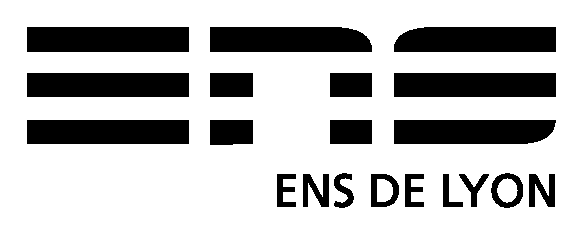
\includegraphics[height=2cm]{logoens.eps} \hfill 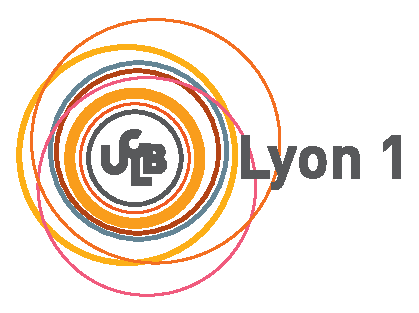
\includegraphics[height=2cm]{logoucbl.eps} \hfill 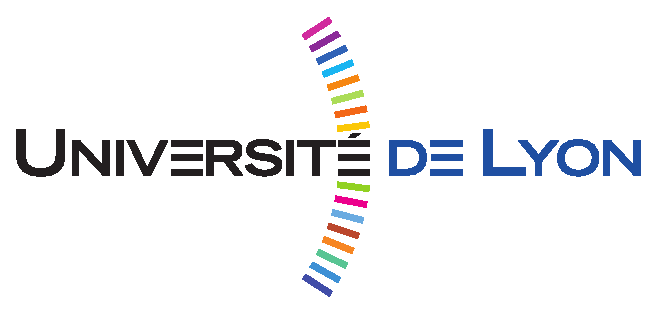
\includegraphics[height=2cm]{logounivlyon.eps}

\vspace{0.5cm}

\begin{tabularx}{\textwidth}{@{} l X l @{} }
{\sc Licence Science de la matière} 	&	& Stage 2022--2023 \\
{\it \'Ecole Normale Sup\'erieure de Lyon}		&	&  \\
{\it Universit\'e Claude Bernard Lyon I}		& 	& L3 Physique
\end{tabularx}

\begin{center}

\vspace{1.5cm}

\rule[11pt]{5cm}{0.5pt}

\textbf{\huge Génération de seconde harmonique}

\rule{5cm}{0.5pt}

\vspace{1.5cm}

\parbox{15cm}{\small
	\textbf{R\'esum\'e}: \it L'équipe de Jérôme Beugnon du groupe Gaz quantiques du Laboratoire Kastler Brossel et du Collège de France, dirigé par Jean Dalibard, manipule des gaz de Bose 2D de rubidium. Le refroidissement et le piègeage des atomes nécessite de nombreux lasers, aux longeurs d'onde adaptées aux différentes transitions atomiques que l'on cherche à exploiter.
 %Les expériences de gaz d'atomes froids utilisent des lasers pour piéger les atomes qui doivent être à des longeurs d'ondes adaptées aux différentes transitions atomiques que l'on cherche à exploiter.
	L'objectif principal de mon stage a été la conception d'un laser à $\SI{532}{\nano\metre}$ (dans le vert) par génération de fréquence double à partir d'un laser infrarouge à 1064 nm. J'ai réalisé l'intégralité du montage et fait varier les différents paramètres disponibles afin d'essayer d'optimiser la puissance et la stabilité du faisceau vert produit. On constate que, du fait des effets thermiques, il est très difficile d'obtenir une puissance stable de l'ordre de quelques watts comme espéré. 
\vspace{0.5cm}
} 


\vspace{0.5cm}

\parbox{15cm}{
\textbf{Mots clefs} : \it optique non-linéaire, génération de seconde harmonique (SHG), niobate de lithium périodiquement polé (PPLN), fibre optique, cristaux photoniques}%TODO

\vspace{0.5cm}

\parbox{15cm}{
Stage encadr\'e par :

{\bf Jérôme \textsc{Beugnon}}

\href{mailto:beugnon@lkb.ens.fr}{\tt beugnon@lkb.ens.fr} / t\'el. (+33) 1 44 27 14 31


Laboratoire Kastler Brossel

{\it Adresse

Postale}

\url{http://adresse.web.du/laboratoire/}
} 

\vspace{0.5cm}


\includegraphics[height=5cm]{./img/logos.png}

%{\tiny \it Logos du laboratoire, de l'universit\'e d'accueil,\\ de l'organisme\ldots (\'eventuellement)}
\end{center}

\vfill
\hfill \today

\end{@empty}

\newpage

\thispagestyle{empty}
\section*{Remerciements}

Je tiens à remercier toute l'équipe Gaz quantiques du Laboratoire Kastler Brossel et du Collège de France pour son accueil chaleureux et pour m'avoir fait découvrir le monde de la recherche de l'intérieur. Je remercie tout particulièrement Franco Rabec pour avoir pris le temps de m'expliquer tous les détails de l'expérience sur laquelle il travaille et Guillaume Brochier pour sa disponibilité, son aide et ses précieux conseils. Je remercie également Benjamin Huard pour m'avoir conseillé ce stage. Enfin, je remercie Jérôme Beugnon, mon maîre de stage, pour sa disponibilité, ses conseils et toutes les connaissances qu'il m'a transmises, ainsi que pour le temps qu'il m'a consacré pendant mon stage mais également en amont pour planifier mon stage et préparer tout le matériel nécessaire. 
\tableofcontents
\newpage


\setcounter{page}{1}


\setlength{\parindent}{16pt}

\section{Introduction}
%Parler du labo, omniprésence des lasers (ralentissement, piègeage, excitation)

%Objectif: lasers IR moins chers et plus robustes -> obtenir du vert par SHG

\subsection{Expériences de rubidium}

La réalisation d'expériences de physique quantique sur des gaz d'atomes nécessite de pouvoir les refroidir jusqu'à des températures en-dessous du kelvin et, souvent, de les piéger dans des potentiels contrôlés. Le refroidissement et le piégeage d'atomes neutres est réalisé avec différentes techniques, parfois combinées ou enchaînées, mais toutes reposant sur l'utilisation de lasers, ce qui explique leur importance cruciale dans ces expériences.

Dans le projet Rubidium du groupe Gaz quantiques (LKB - Collège de France), les atomes refroidis et piégés par une séquence de piège magnéto-optique (MOT), de pièges magnétique et optique et de refroidissements par évaporation, que nous ne discuterons pas ici, sont ensuite confinés dans un plan pour former un gaz dégénéré à 2 dimensions avec de l'ordre de $10^5$ atomes à \SI{20}{nK}. Comme expliqué dans la sous-section suivante, un laser vert (à \lmbd{532}) pousse les atomes de rubidium vers un minimum d'intensité. 
Ainsi, en éclairant le nuage d'atomes avec un faisceau vert (vertical sur la figure) dont le profil, réalisé avec un DMD (\textit{digital mirror device}) est en forme d'anneau, on réalise une ``boîte'' circulaire avec un puits de potentiel plat dans laquelle les atomes sont confinés. Pour geler le degré de liberté vertical, on fait interférer deux faisceaux cohérents inclinés pour réaliser une figure d'interférence constituée de franges planes, comme on peut le voir figure \ref{fig:accordeon} (les 2 faisceaux en question sont les faisceaux vert clair sur la figure), et on confine les atomes dans un des minima. Pour ce faire, on commence par piéger l'intégralité des atomes dans un même minimum d'intensité en créant une figure avec une interfrange large, puis on resserre progressivement l'interfrange en faisant varier l'inclinaison des faiceaux. En forçant une évaporation optique, on ne garde que les atomes moins énergétiques de sorte qu'à la fin de la séquence expérimentale, l'intégralité des atomes soit dans le mode fondamental du puits. Les atomes ont alors une fonction d'onde gaussienne d'épaisseur de l'ordre de \lmbd{180} \citep{brice}. On voit figure \ref{fig:accordeon} en bleu une image des atomes piégés dans le disque. Un deuxième DMD avec un nouveau laser vert peuvent alors être utilisés pour façonner différents potentiels à l'intérieur de la ``boîte''.

\begin{figure}[htbp] 
	\centering
	%
	\begin{subfigure}[b]{0.48\textwidth}
    	\centering
    	\small
	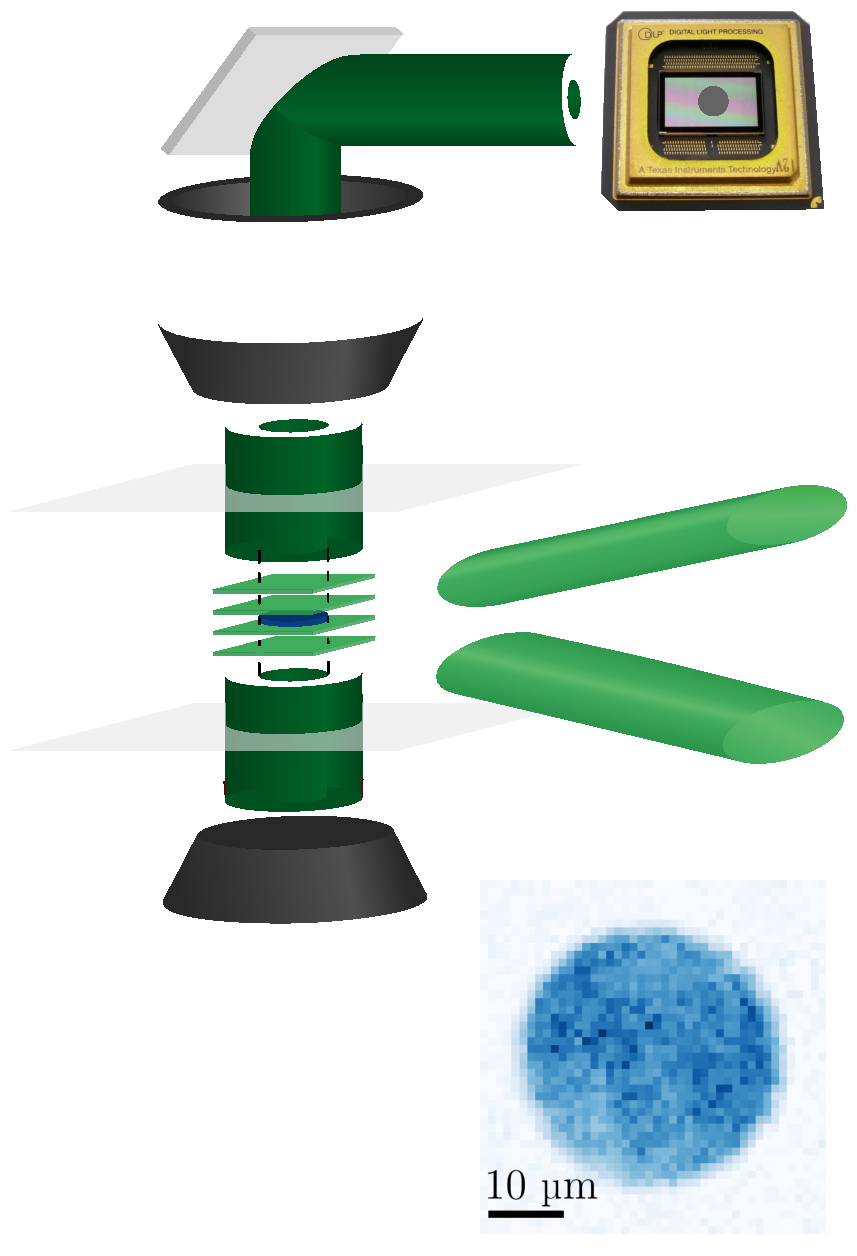
\includegraphics[height=9cm]{img/accordeon-dmd.pdf}
	\caption{\small Réalisation d'un piège circulaire 2D \ncite{ville}} %\footnotemark}
		\label{fig:accordeon}
	\end{subfigure}	
	%
	\begin{subfigure}[b]{0.48\textwidth}
		\centering
		\small
		\resizebox{!}{9cm}{
   			\begin{tikzpicture}[
level/.style = {
        ultra thick,
        red,
    },
    laser/.style = {
        ultra thick,
        green,
        dashed
    },
    connect/.style = {
        dashed,
        red
    },
    trans/.style={thick,->,shorten >=2pt,shorten <=2pt,>=stealth},
    notice/.style = {
        draw,
        rectangle callout,
        callout relative pointer={#1}
    },
    label/.style = {
        text width=2cm
    }
]
    % Draw all levels
    \draw[level] (0,0) --  +(-2,0) node[left] {$3S^{1/2}$} ;
    \draw[level] (0,4) --  +(-2,0) node[left] {$3P^{1/2}$} ;
    \draw[level] (0,4.5) --  +(-2,0) node[left] {$3P^{3/2}$};
    \draw[laser] (0,6) --  +(-2,0) node[left] {laser};
    
    \draw[trans] (-1.1,0) -- +(0,4) node[pos=0.4,left] {794.8 nm}; %794.8
    \draw[trans] (-1,0) -- +(0,4.5) node[pos=0.6,left] {780.0 nm}; %780.0
    \draw[trans] (-0.5,0) -- +(0,6) node[pos=0.85,left] {532 nm};
    
\end{tikzpicture}

		}
		\caption{\small Transitions du rubidium 87}
		\label{fig:transitions}
	\end{subfigure}
	%

	\caption{Utilisation du laser à \lmbd{532} dans l'expérience : \small le laser est à une fréquence très supérieure à celle des transitions du rubidium 87, ce qui permet de piéger les atomes dans les minima d'intensité}
\end{figure}

%\footnotetext{schéma extrait de la thèse de Brice Bakkali-Hassani, ancien doctorant sur l'expérience}


\subsection{Utilisation des lasers à 532 nm}

Alors que le refroidissement des atomes se fait avec des lasers résonants, c'est-à-dire de fréquence proche de celle de la transition visée, et repose sur l'échange d'impulsion lors de l'absorption et la réémission de photons, le piégeage est réalisé avec des lasers non-résonants, désaccordés soit vers le rouge (\textit{i.e.} de fréquence très inférieure à celle des transitions atomiques), soit vers le bleu (\textit{i.e.} de fréquence très supérieure à celle des transitions atomiques), et repose sur le principe du piégeage optique dipolaire exploitant l'interaction champ électrique - dipôle électrique induit.

C'est le cas des lasers à \lmbd{532}, qui sont désaccordés vers le bleu pour le rubidium 87 comme on peut le voir sur le diagramme des transitions figure \ref{fig:transitions}.

Cette interaction donne lieu, classiquement, à une force dérivant du potentiel $U_\mathsc{dip}(\v r) = {-\frac12 \langle \v d \cdot \v E \rangle} = -\frac{1}{2\varepsilon_0 c}\mathfrak{Re}\left(\alpha(\omega)\right) I(\v r)$ ($\v d$ désigne le moment dipolaire induit, $\alpha$ la polarisabilité complexe, $\langle \cdot \rangle$ une moyenne temporelle et $I$ l'intensité du faisceau)
%\footnote{Le facteur $\frac12$ est dû au fait que le dipôle est non pas permannent mais proportionnel au champ appliqué.} %En effet, pour $\v d = \alpha \v E$, $\v F = (\v d \cdot \v \nabla) \v E = \frac12 \v \nabla (\v d \cdot \v E)$}  %
qui va servir à piéger les atomes dans un minimum de potentiel. Le rayonnement laser va également engendrer des cycles d'absorption et réémission spontanée, ayant lieu, toujours ``classiquement'', à une fréquence $\Gamma_\mathsc{diff} = \frac{P_\mathsc{abs}}{\hbar \omega} = \frac{1}{\hbar \varepsilon_0 c} \mathfrak{Im}\left(\alpha(\omega)\right) I(\v r)$ où $P_\mathsc{abs} = \langle \dot{\v d} \cdot \v E \rangle$ est la puissance absorbée par l'atome, qui vont conduire à un réchauffement des atomes. 
Pour un atome à deux niveaux avec une transition à $\omega_0$, dans l'approximation de faible saturation (état excité faiblement peuplé) et de fort désaccord ($\Delta = \omega - \omega_0$ vérifiant $|\Delta| \ll \omega_0$), vérifiée en pratique et permettant de justifier le calcul classique (à une précision de l'ordre du pourcent), on trouve
\vspace{-0.2cm}
\begin{align}
	U_\mathsc{dip}(\v r)&=\frac{3\pi c^2}{2\omega_0^3} \frac{\Gamma}{\Delta} I(\v r) \\
	\Gamma_\mathsc{diff}(\v r)&=\frac{3\pi c^2}{2\hbar\omega_0^3} \left(\frac{\Gamma}{\Delta}\right)^2 I(\v r) 
\end{align}

avec $\Gamma = \frac{\e 2 \omega^2}{6 \pi \varepsilon_0 m_e c^3}$ la largeur naturelle de la transition, qui correspond dans une vision classique au facteur d'amortissement dû au rayonnement.

Puisque $\Gamma_\mathsc{diff}=\frac{\Gamma}{\hbar \Delta} U_\mathsc{dip}$, on voit qu'un grand désaccord permet de minimiser le chauffage dû à la diffusion. On remarque également que pour un faisceau laser désaccordé vers le rouge, l'atome est piégé dans les zones lumineuses, alors que pour un désaccord vers le bleu, l'atome est piégé dans les zones sombres.

Pour un atome réel à plusieurs niveaux, l'énergie d'interaction (qui s'obtient plus rigoureusement en considérant la perturbation par un hamiltonien de couplage $\mathcal H_1 = - \hat{\v d} \cdot \v E$ des états propres du système atome + champ) est la somme des contributions des différents états excités, pondérée par l'importance des transitions associées \citep{grimm}. Pour les atomes de rubidium 87 utilisés dans l'expérience, les transitions prépondérantes sont les 2 transitions de la ligne D qui sont représentées figure \ref{fig:transitions}.


\subsection{Objectif du stage}

Les lasers verts actuellement utilisés au laboratoire sont des lasers à \lmbd{1064} Nd-Yag ``solides'' ou des lasers à fibres qui sont vendus directement avec le doublage de fréquence. Ils ont l'inconvénient d'être particulièrement onéreux et fragiles, et leur réparation nécessite plusieurs mois d'attente. L'objectif de mon projet était donc d'explorer la possibilité de réaliser le doublage soi-même à partir d'un laser à \lmbd{1064} beaucoup plus facile d'accès. Ce doublage de fréquence (SHG pour \textit{second harmonic generation} en anglais) repose sur l'existence d'un terme dans la polarisation électrique de certains cristaux quadratique en le champ appliqué, qui joue le rôle d'un terme source à la fréquence double de celle du faisceau incident. C'est notamment le cas du niobate de lithium choisi pour ce projet. %Le principe sera expliqué plus en détail section \ref{SHG}. 

\section{Couplage de la fibre à cristaux photoniques}
Une première partie de mon stage, indépendante de l'objectif principal d'obtenir un laser vert, a été de tester une fibre à cristaux photoniques
%, plus précisément une fibre de verre à trous (\textit{holey fiber}) 
LMA-PM-10 de la marque NKT Photonics. LMA signifie large (effective) mode area et donc que la fibre est faite pour des faisceaux larges, ce qui est important pour les applications avec des lasers de plusieurs dizaines de watts, car le seuil de destruction des matériaux ainsi que les effets thermiques dus à la dissipation dépendent de l'intensité et non de la puissance totale. La fibre utilisée a un mode de $\SI{8.6}{\micro\meter}$ de diamètre alors que les fibres traditionnelles ont plutôt un diamètre de $\SI{3}{\micro\meter}$. L'utilisation d'une fibre à cristaux photoniques LMA permet donc de réduire l'intensité de presque un ordre de grandeur.

La technologie des fibres optiques traditionnelles, reposant sur une réflexion interne totale, ne permet pas de fabriquer des fibres à c\oe ur large qui resteraient monomodes sur une gamme de longueurs d'ondes et de rayon de courbure de la fibre suffisante. 
Les fibres à cristaux photoniques, quant à elles, reposent sur une variation d'indice optique effectif périodique grâce à une structure régulière de trous et ont l'avantage de permettre beaucoup plus de liberté, notamment en terme de taille du c\oe ur tout en restant monomodes, et ce sur une très large gamme de fréquences.  
%Cette structure conduit à des bandes interdites analogues à celles des électrons dans un crystal (ondes de Bloch). 
\citep{russell2006,russell2007}

%Contrairement aux fibres traditionnelles, la variation d'indice optique dans ces fibres est réalisée à l'aide d'une structure régulière de trous. En effet, l'air aillant un indice optique inférieur au matériau de la fibre, les trous permettent de réduire l'indice moyen. % TODO: corriger

\begin{figure}[htpb]  
\centering
\hspace*{0.4cm}
\begin{subfigure}[t]{0.38\textwidth}
	\centering
	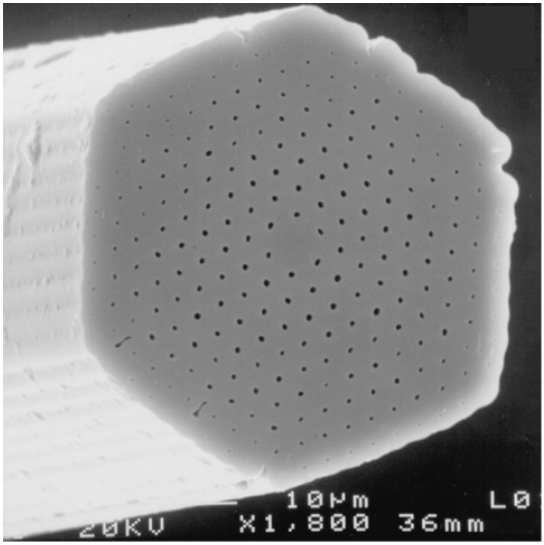
\includegraphics[height=5.3cm]{../biblio/solid core PCF - russell2006}
	\caption{Image par microscopie électronique par balayage de la première fibre à cristaux photoniques fonctionnelle \ncite{russell2006}}
	\label{fig:PCF}
\end{subfigure}
\hspace*{0.4cm}
\begin{subfigure}[t]{0.37\textwidth}
	\centering
	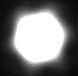
\includegraphics[height=5.3cm]{./img/mode hexa.png}
	\caption{Image en intensité du mode hexagonal en sortie (caméra fortement saturée)}
	\label{fig:hexa}
\end{subfigure}
\hspace*{-0.8cm}
\caption{Structure de la fibre à cristaux photoniques et mode hexanogal en sortie}
\end{figure}

Comme indiqué, la fibre à cristaux photoniques ne sélectionne qu'un seul mode. Les fibres monomodes traditionnelles sélectionnent généralement un mode gaussien, mais la géométrie de la fibre à cristaux photoniques utilisée fait que le mode sélectionné est un mode hexagonal, comme on peut le voir figure \ref{fig:hexa}. Ce mode ne se distingue cependant que très peu d'un mode gaussien, et on ne voit la forme hexagonale qu'en saturant la caméra.

En particulier, afin de maximiser la transmission de la fibre, il faut que l'axe de propagation du faisceau incident (gaussien) coïncide avec celui de la fibre, ce qui correspond à l'ajustement de 4 paramètres (2 angles pour l'orientations et 2 coordonnées pour la position dans le plan transverse). L'ajustement est fait à l'aide de 2 miroirs (cf schéma figure \ref{fig:couplage}). Il faut également que le faisceau ait le bon waist et qu'il soit focalisé en bout de fibre. La focalisation est réalisée à l'aide d'un coupleur de fibre (60SMS-SMA-0-M5-08 de la marque Schäfter+Kirchhoff), qui est un collimateur de focale 5 mm optimisé pour le couplage de fibres et nécessite de produire un faisceau collimaté en amont du coupleur avec le bon waist (que l'on peut déterminer expérimentalement en observant le faisceau en sortie de fibre, puisqu'elle est équipée d'un coupleur identique). Cet ajustement est fait à l'aide d'un téléscope avec des focales adaptées.

\begin{figure}[h]
	\centering
	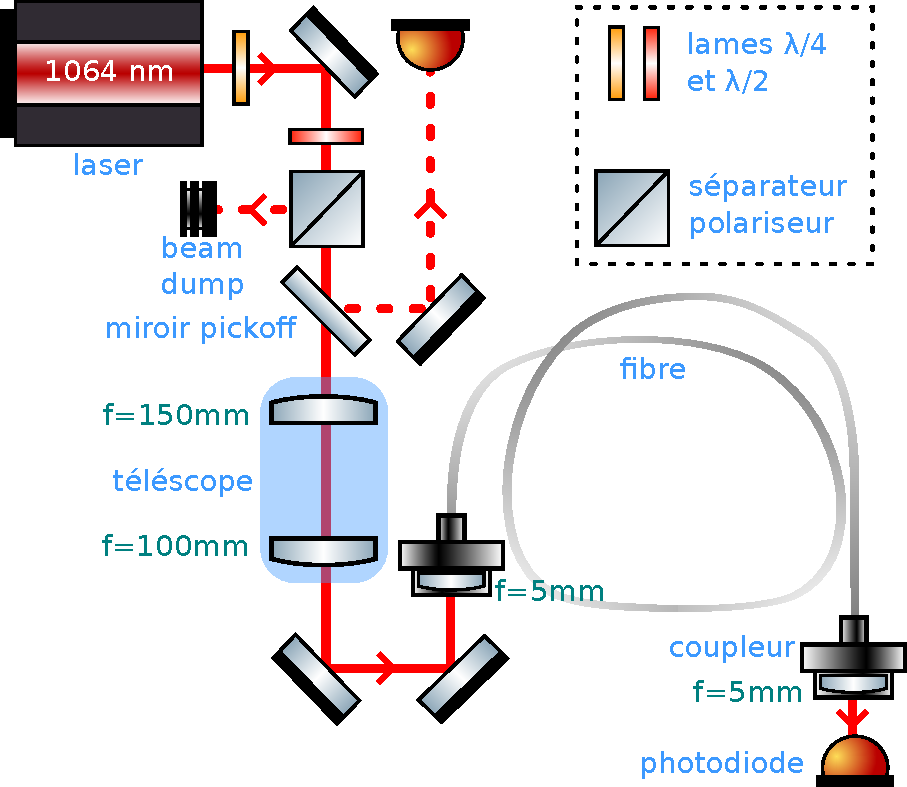
\includegraphics[width=0.7\textwidth]{./img/schema couplage.pdf}
	\caption[Montage de la fibre à cristaux photoniques]{Montage de la fibre à cristaux photoniques :
	\small Le cube séparateur permet de sélectionner une polarisation linéaire, et les lames d'onde servent à maximiser la composante du champ selon la direction transmise afin de minimiser les pertes. La composante réfléchie finit dans un ``beam dump'', fait pour absorber le rayonnement infrarouge et dissiper la chaleur. Le ``pickoff'', lame de verre avec un traitement adapté, sert à réfléchir une petite partie du faisceau pour l'envoyer sur une photodiode. Une calibration permet de corréler la tension sur la photodiode à la puissance en sortie du séparateur. Le téléscope, de grandissement $\gamma = \frac{100}{150} = 0.67$, sert à produire un faisceau collimaté avec le waist souhaité, et enfin le coupleur d'entrée de fibre sert à adapter le faisceau incident à la fibre. Le coupleur de sortie sert à obtenir un faisceau collimaté et plus large qu'au sein de la fibre. Une deuxième photodiode permet de mesurer la puissance transmise et évaluer l'efficactié du couplage.}
	\label{fig:couplage}
\end{figure}

De façon plus détaillée, le protocole du couplage est essentiellement le suivant :
\begin{enumerate}
	\item On choisit une hauteur de faisceau avec laquelle on va trailler, et on aligne la source laser et les optiques à cette hauteur.
	\item À l'aide des vis des 2 miroirs réglant l'angle vertical, on assure l'horizontalité et la bonne hauteur du faisceau par rapport au collimateur en faisant passer le faisceau à travers ce dernier.
	\item On connecte la fibre au collimateur. Si l'alignement est bon, on doit avoir une puissance mesurable en sortie.
	\item Pour déterminer le waist adapté à la fibre et au coupleur, on utilise la présence d'un coupleur identique à l'autre extrémité de la fibre. En effet, le faisceau gaussien en sortie aura, par retour inverse de la lumière, le bon waist à injecter dans la fibre. Le waist du mode en sortie est déterminé par la mesure à la caméra du diamètre du faisceau à différentes positions.	
	\item On monte un téléscope avec un grandissement permettant d'obtenir le waist voulu.
	\item On alterne optimisation de la position du collimateur et de l'alignement. Il faut se méfier que le déplacement du collimateur affecte l'alignement.
	\item L'alignement s'effectue selon la méthode du `beam-walk' : les rotations des 2 miroirs selon le même axe ont un effet couplé, permettant par exemple d'induire une translation pure du faisceau. Il est donc préférable de faire varier un angle et trouver le maximum pour cet angle en faisant varier l'angle associé sur le deuxième, et comparer ces maxima successifs. En effet, le couplage est sensible même aux petites variations d'angle, mais les maxima successifs obtenus en `beam-walkant' sont assez proches. 
\end{enumerate}

J'ai ainsi pu obtenir un couplage d'environ $\SI{75}{\percent}$, ce qui est tout à fait raisonnable. En particulier, on peut injecter $\SI{10}{W}$ dans la fibre sans risquer de l'endommager du fait d'une trop forte dissipation de puissance.

TODO: injection en pola


\section{Principe de la génération de seconde harmonique (SHG)} %\'Etude th\'eoriqaue de la génération de seconde harmonique (SHG)}
\label{SHG}

Nous revenons maintenant à l'objectif principal du stage, l'obtention d'un laser à \lmbd{532} par génération de seconde harmonique, dont nous expliquons d'abord le principe.

\subsection{Polarisation non linéaire et seconde harmonique}

\begin{figure}[h]
\centering
\begin{subfigure}{0.45\textwidth}
	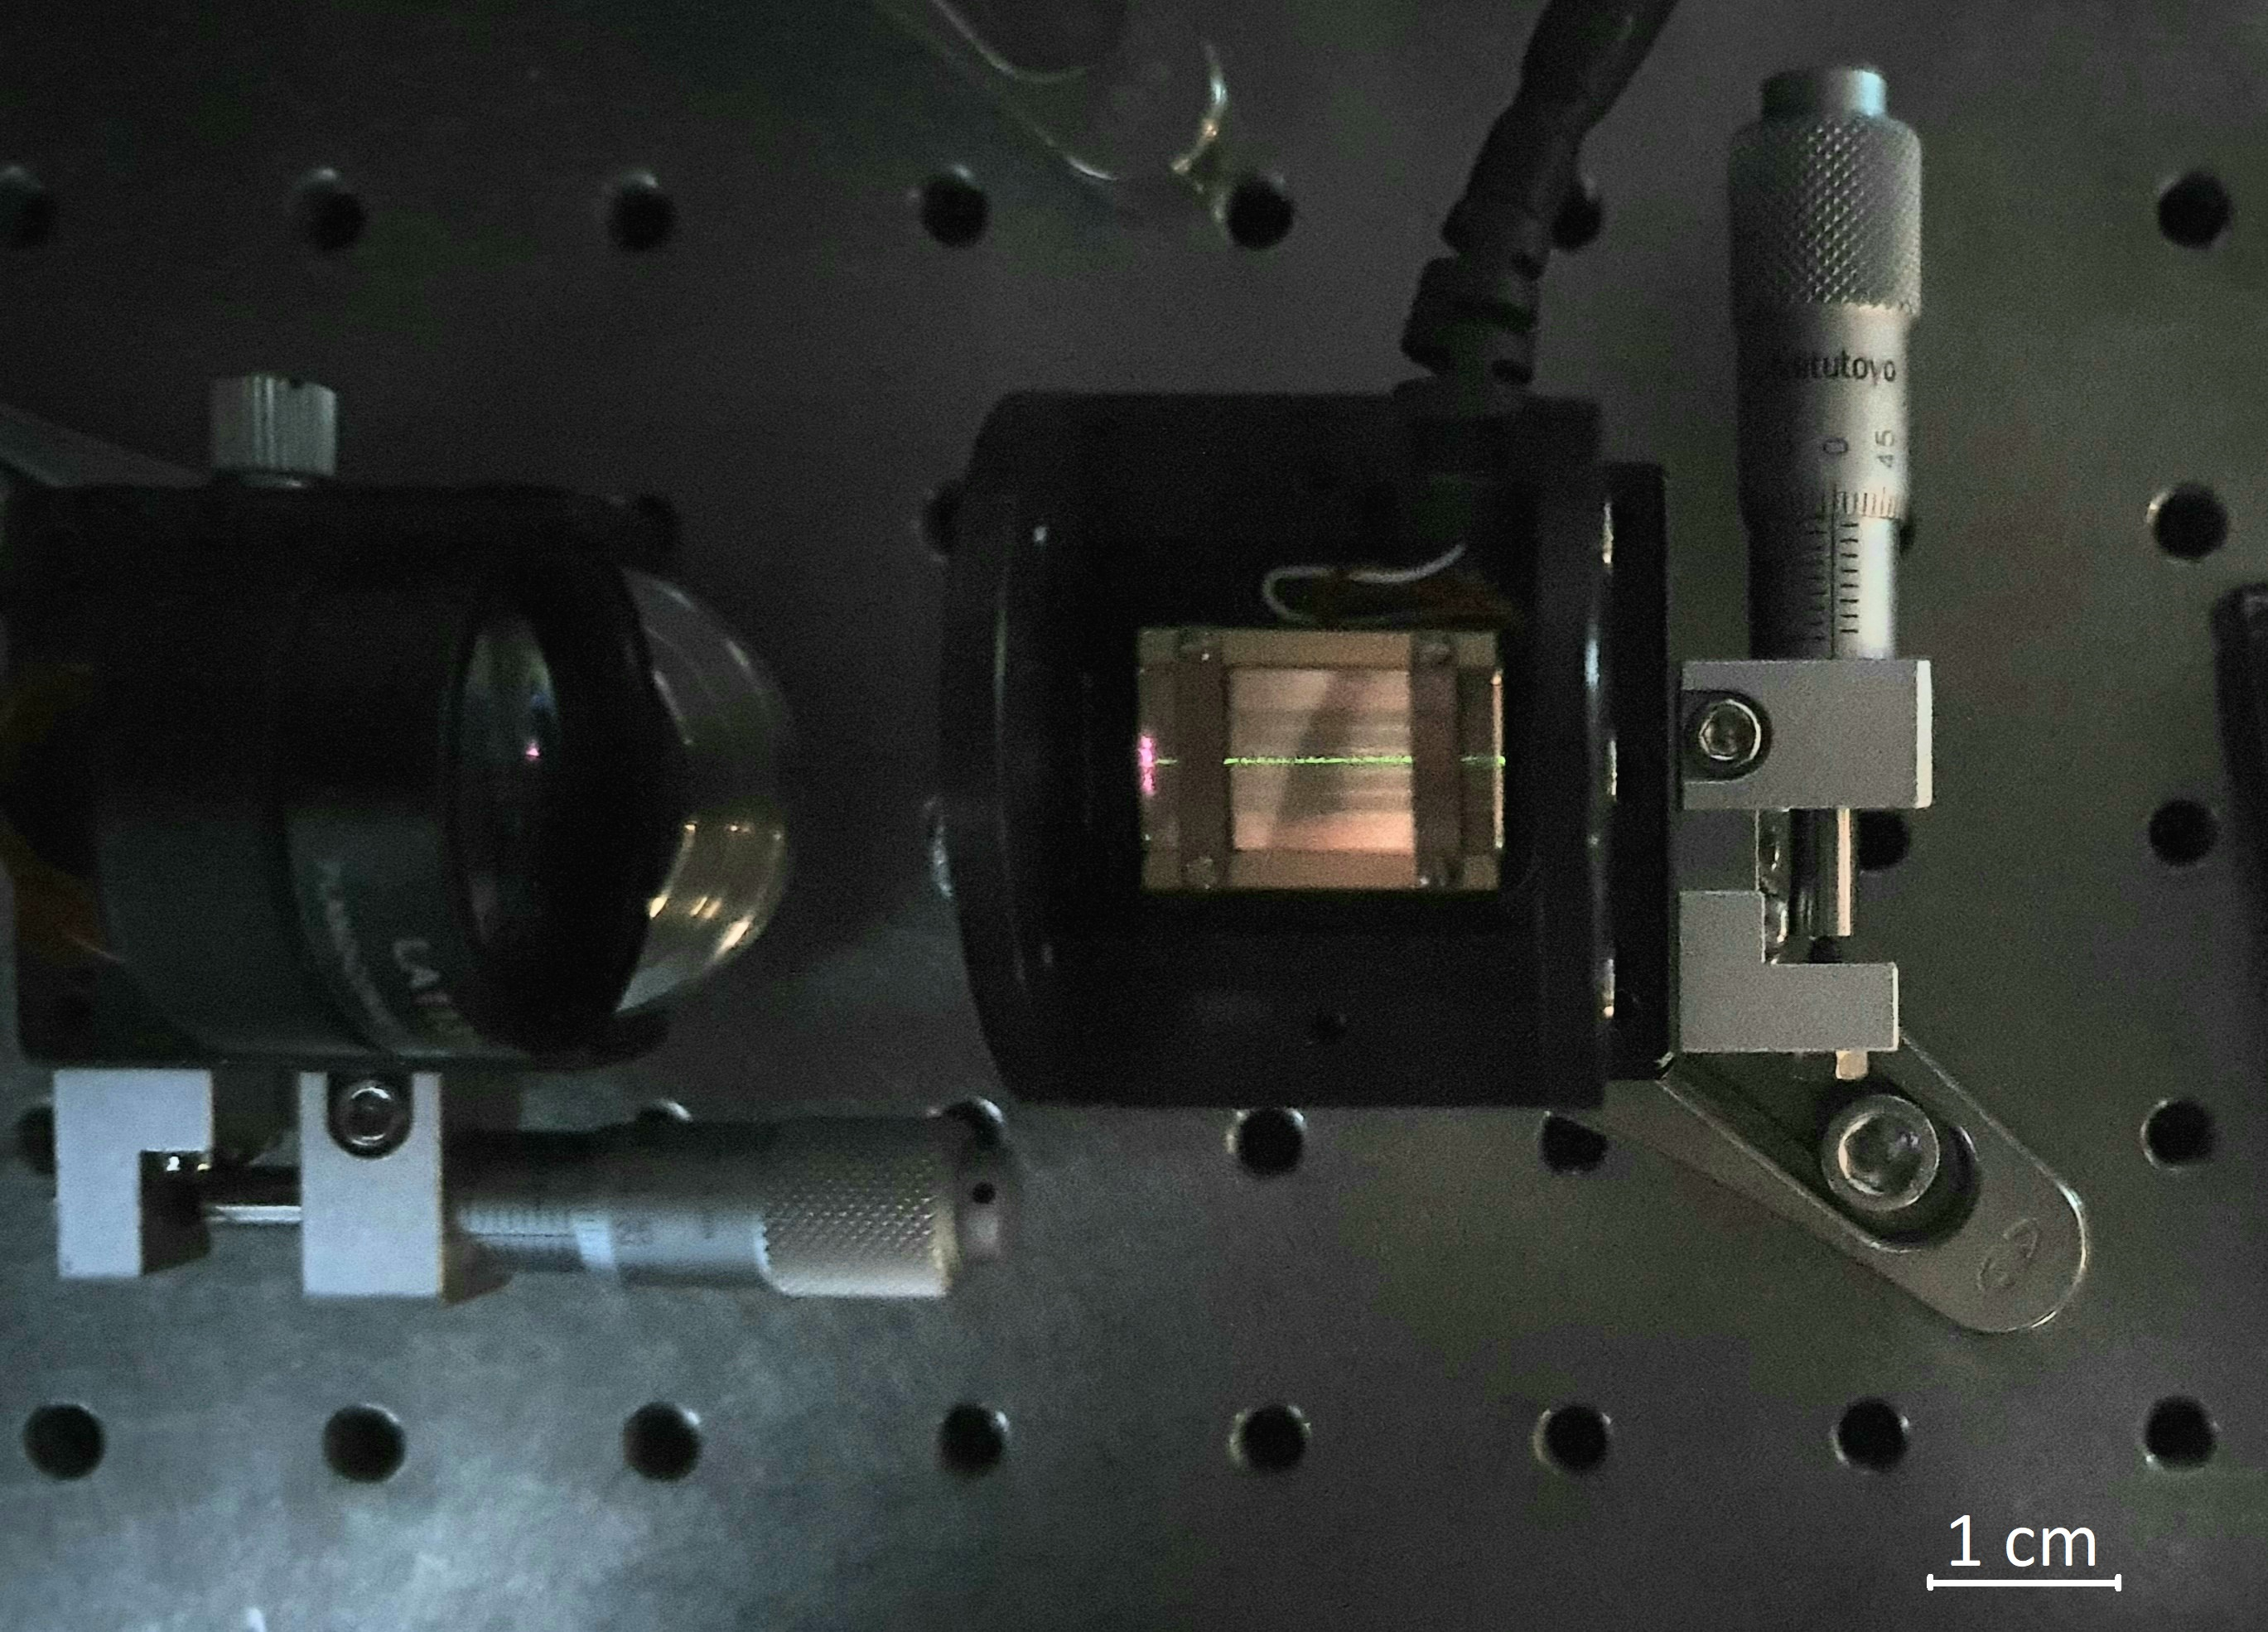
\includegraphics[width=\textwidth]{./img/cristal clair.jpg}
\end{subfigure}
\begin{subfigure}{0.5\textwidth}
	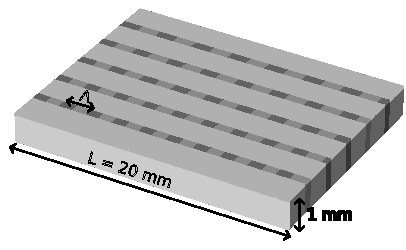
\includegraphics[width=\textwidth]{./img/cristal.pdf}
\end{subfigure}
\caption{Génération d'un laser vert dans un cristal doubleur de fréquence : \small le faisceau incident passant par une des bandes avec une structure de période $\Lambda$, dont le rôle est expliqué section \ref{qpm}, donne lieu à un faisceau vert grâce à la polarisation d'ordre 2 du cristal}
\label{fig:cristal}
\end{figure}

La génération de la seconde harmonique a lieu dans un cristal doubleur de fréquence avec des propriétés non-linéaires favorables (figure \ref{fig:cristal}).
La propagation d'ondes électromagnétiques dans un milieu non linéaire non magnétique donne lieu à une équation d'onde avec un terme source, qui s'écrit 
\begin{align}
\boldsymbol{\nabla}^2 \boldsymbol{\E}_q + \frac{\omega_q^2}{c^2}\tens\epsilon^{(1)}(\omega_q)\cdot \v \E_q(\v r) = - \frac{\omega_q^2}{\epsilon_0 c^2} \boldsymbol{\mathcal{P}}^\mathsc{NL}_q(\v r)
\end{align}
dans le domaine de Fourier en temps avec la convention $\v E(\v r, t) = \mathfrak{Re} \left\{ \sum_{q \in \mathbb N} \v {\boldsymbol{\mathcal E}}_q (\v r) \e{-i \omega_q t} \right\}$ et $\v P^\mathsc{NL} (\v r, t) = \mathfrak{Re} \left\{ \sum_{q \in \mathbb N} \v {\boldsymbol{\mathcal P}}^\mathsc{NL}_q (\v r) \e{-i \omega_q t} \right\}
$,
%, avec n un indice désignant la composante spectrale (il s'agira dans notre cas de l'ordre de l'harmonique), 
avec $\tens \epsilon^{(1)}$ le tenseur de permittivité diélectrique relative associé à la partie linéaire de la polarisation et $\v P^\mathsc{NL}_q$ la partie non-linéaire de la polarisation (cf annexe \ref{NL}) \ncite{boyd,joffre}.

On fait l'hypothèse simplificatrice d'une \textbf{polarisation linéaire} selon un des axes principaux et on travaillera par la suite avec des $\mathcal E_q$ scalaires. En particulier, la permittivité tensorielle $\tens \varepsilon^{(1)}$ est remplacée par sa valeur propre correspondante et donne lieu à un indice optique $\boxed{ n_q = \sqrt{ \varepsilon^{(1)}(\omega_q)}}$. En écrivant les différentes harmoniques sous la forme d'une ``onde monochromatique d'amplitude variable'' $\mathcal E_q = \A_q(x,y,z) \e{ik_qz}$ avec $\boxed{k_q =\frac{n_q \omega_q}{c}}$ et en se plaçant dans l'approximation paraxiale, i.e. de lente variation de $\A$ avec $z$ $\left(\frac{\partial^2 \A_q}{\partial z^2} \ll k_q \frac{\partial \A_q}{\partial z}\right)$, on arrive aux équations \ncite{joffre}
\begin{align}  
	\left\{\v\nabla_\bot + 2 i k_q \frac{\partial}{\partial z} \right\} \A_q = - \frac{\omega_q^2}{\varepsilon_0 c^2} \v P^\mathsc{NL}_q (\v r) \e{-ik_qz}
	\label{eq:parax}
\end{align}
avec $\v\nabla_\bot = \pdv{}{x^2} + \pdv{}{y^2}$.

En particulier, pour un champ électrique avec une composante à $\omega$ et une à $2\omega$, le terme quadratique dans la polarisation est donné par \ncite{joffre}
\begin{equation}
\begin{aligned}
	P^{(2)} &= \varepsilon_0 \chi^{(2)} \v E^2  \text{ avec $\chi^{(2)}$ la susceptibilité d'odre 2}\\
	&= \frac{\varepsilon_0 \chi^{(2)}}{4} \left\{\mathcal E_1 e^{-i\omega t} + \mathcal E_1^* e^{i\omega t} + \mathcal E_2 e^{-2i\omega t} + \mathcal E_2^* e^{2i\omega t} \vphantom{\frac12}\right\}^2 \\
	&= \frac{\varepsilon_0 \chi^{(2)}}{4} \left\{\mathcal E_1^2 \e{-2i\omega t} + \E_1^{*2} \e{2i\omega t} + 2|\mathcal E_1|^2 + 2 \E_1\E_2^* \e{i\omega t} + 2 \E_1^*\E_2 \e{-i\omega t} \vphantom{\frac12}\right. \\
	&\qquad\qquad\qquad \left. + 2 \E_1\E_2 \e{-3 i\omega t}  + 2 \E_1^*\E_2^* \e{3 i\omega t} + \mathcal O(\E_2^2) \vphantom{\frac12}\right\} \\ 
%	&= \mathfrak{Re} \left\{ \sum_{q \in \mathbb N} \v {\boldsymbol{\mathcal P}}^{(2)}_q \e{-i \omega_q t} \right\}
\end{aligned}
\end{equation}
où l'on a considéré que $\chi^{(2)}$ est approximativement le même pour toutes les harmoniques. 
% où l'on a considéré que $\chi^{(2)}$ est le même pour toutes les harmoniqes pour un milieu supposé sans pertes \ncite{boyd}.

On voit donc que l'onde incidente (à $\omega$) conduit à un terme à la fréquence double dans la polarisation, qui va conduire à la création d'une onde à cette seconde harmonique comme souhaité. Cette dernière va conduire à un terme à la fréquence fondamentale qui va affecter l'onde incidente ainsi qu'à un terme à la fréquence triple qui va conduire à une onde à la troisième harmonique et ainsi de suite. 
Dans l'hypothèse où la seconde harmonique est d'amplitude faible par rapport au faisceau incident, nous pouvons cependant négliger ces termes d'ordre supérieur. Cette hypothèse, connue sous le nom \textbf{d'hypothèse de non-déplétion}, est discutée en annexe \ref{ndepl}. Nous négligerons également le terme constant dit de redressement. %Nous nous plaçons cependant dans l'hypothèse que la seconde harmonique 

%En écrivant les différents champs 

%Plus précisément, en écrivant les équations d'onde paraxiales pour les différentes harmoniques, 

Ceci conduit à l'équation d'évolution de l'amplitude de l'onde générée $\A_2$ suivante:
\begin{align}
	\left\{\v\nabla_\bot + 2 i k_2 \frac{\partial}{\partial z} \right\} \A_2 = - \frac{2 \chi^{(2)} \omega^2}{c^2} \A_1^2 \e{- i (k_2 - 2k_1) z}
	\label{eq:SHG}
\end{align}

\subsection{Le problème de l'accord de phase}
\label{qpm}
Cette équation est beaucoup plus abordable dans l'approximation d'une onde plane avec $\A_1$ et $\A_2$ ne dépendant que de $z$ (et donc $\A_1$ constante dans \textbf{l'hypothèse de non-déplétion}):
\begin{align}
	\dv{\A_2}{z} &= i\frac{\chi^{(2)}\omega}{2cn_2} \A_1^2 \e{-i \Delta k z} \text{ avec } \boxed{\Delta k = k_2 - 2k_1} \label{eq:pwe} \\
	\text{soit } \A_2(L) &= i \frac{\chi^{(2)}\omega}{2 cn_2} \A_1^2 L \operatorname{sinc}\left( \frac{\Delta k L}{2} \right) \e{-i\frac{\Delta k L}{2}}
\end{align}
en sortie du cristal en $z=L$ avec $\A_2(0)=0$ à l'entrée.

Cette équation se comprend très bien en considérant que le carré de l'onde incidente, de nombre d'onde $2k_1$, génère un rayonnement qui se déplace ensuite à $k_2$, de sorte qu'en un point $z$ une onde de phase $2k_1z$ vient s'ajouter à une onde se propageant avec un nombre d'onde $k_2$. Ainsi, l'onde à la seconde harmonique générée en $z$ aura à la sortie du cristal en $z=L$ la phase $2k_1 z + k_2 (L-z) = k_2 L - \Delta k z$ (modulo une constante universelle), de sorte que les ondes générées en $z$ et en $z+L_\mathsc{coh} := z + \frac{\pi}{\Delta k}$ interfèrent destructivement, ce qui conduit à une amplitude nulle en sortie, comme illustré figure \ref{fig:agen}.

\begin{figure}[htpb] 
\centering
\begin{subfigure}[b]{0.48\textwidth}
	\centering
	\hspace*{-0.8cm}
	%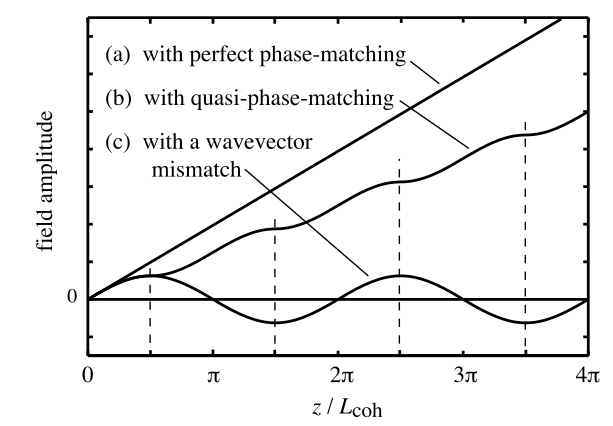
\includegraphics[height=5cm]{./img/QPM.png}
	\include{./img/qpm.tex}
	\vspace*{-1cm}
	\caption{}
	\label{fig:agen}
\end{subfigure}
\begin{subfigure}[b]{0.48\textwidth}
	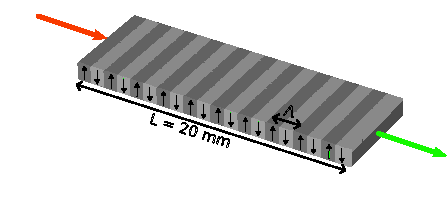
\includegraphics[height=4cm]{./img/PP.pdf}
	\vspace*{0.8cm}
	\caption{}
	\label{fig:inversion}
\end{subfigure}
\hspace*{-0.6cm}
\caption{Amplitude de seconde harmonique et quasi-accord de phase : (a) \small  Sans accord de phase, l'amplitude de la seconde harmonique retombe à zéro toutes les $2L_\mathsc{coh}$ et la croissance linéaire avec la longueur du cristal est perdue. La technique du quasi-accord de phase permet de la retrouver, bien qu'avec un coefficient plus faible. (b) L'inversion de polarisation tous les $\Lambda/2$ permet la réalisation du quasi-accord de phase.} %TODO
\label{fig:QPM}
\end{figure}

Avec le cristal de niobate de lithium utilisé, $L_\mathsc{coh}$ vaut à peine $\SI{3}{\micro\meter}$ alors que le cristal fait $\SI{2}{cm}$.
Afin d'avoir une génération efficace, il faudrait donc $\Delta k = \frac{2\pi}{\lambda_2}(n_2-n_1) = 0$ (condition d'accord de phase) avec $\lambda_2=$\lmbd{532} la longueur d'onde dans le vide de la seconde harmonqiue, soit $n_2 = n_1$. Cela n'est \textit{a priori} pas possible sans dispersion anormale. Une solution consiste alors à exploiter la biréfringence du cristal, mais cette méthode est difficile à réaliser et le $\chi^{(2)}$ correspondant à la polarisation requise est souvent assez faible. 

Nous avons choisi une autre solution qui consiste à fabriquer un cristal dont le $\chi^{(2)}$ varie spatialement. En effet, si $\chi^{(2)}(z) = \chi^{(2)}_0 \e{i k_\chi z}$, cela revient à remplacer $\Delta k$ par $\boxed{ \Delta k_\mathsc{eff} = \Delta k - k_\chi }$ dans (\ref{eq:pwe}). 
%En pratique, il est difficile de fabriquer un tel cristal, et on préfère inverser le signe de $\chi^{(2)}$ en inversant l'axe extraordinaire d'un matériau ferroélectrique avec une période $\Lambda$ (cf figure \ref{fig:QPM}). 
Évidemment, la susceptibilité est en réalité proche d'une valeur réelle et un tel $\chi^{(2)}$ n'est pas réalisable. À la place, on inverse le signe de $\chi^{(2)}$ en inversant l'axe extraordinaire d'un matériau ferroélectrique avec une période $\Lambda$ (cf figure \ref{fig:inversion}) \footnote{En effet, si $P_z = \chi^{(2)} E_z^2$ et on change $P_z$ et $E_z$ de signe, on voit que $\chi^{(2)}$ est changé en son opposé.}.
On parle alors de quasi-accord de phase et un tel cristal est dit périodiquement pôlé. Dans ce cas, la décomposition de Fourier de $\chi^{(2)}(z) = \chi^{(2)}_0 \operatorname{sgn}[\cos(2\pi z/ \Lambda)]$ montre que le terme de plus grande amplitude est le fondamental d'amplitude $\boxed{ \chi_\mathsc{eff} = \frac2\pi \chi^{(2)}_0 }$ et de nombre d'onde $\boxed{ k_\chi = \frac{2\pi}{\Lambda} }$. 
Si $k_\chi = \Delta k$, $\Delta k_\mathsc{eff} = 0$ et le terme source correspondant sera accordé en phase sur toute la longueur du cristal et permettra donc de générer la seconde harmonique. Par la suite, on ne tiendra compte que de ce terme, oubliant les autres harmoniques de $\chi^{(2)}(z)$ (cela correspond à la ligne en pointillés, qui approxime bien la courbe orange).
Ceci nous conduit à une amplitude 
\begin{align}
	\A_2(L) &= i \frac{\chi_\mathsc{eff}\omega}{2 cn_2} \A_1^2 L \operatorname{sinc}\left( \frac{\Delta k_\mathsc{eff} L}{2} \right) 
	\e{-i\frac{\Delta k_\mathsc{eff} L}{2}} \\	
	&= i \frac{\chi_\mathsc{eff} \omega}{2 cn_2} \A_1^2L 
\end{align}
si le quasi-accord de phase est respecté.

Ainsi, l'intensité de la seconde harmonique est quadratique en l'intensité du fondamental avec
\begin{align}
	\frac{\mathcal I_2}{\mathcal I_1^2} &= \frac{\frac12 n_2 \varepsilon_0 c |\A_2|^2}{\left(\frac12 n_1 \varepsilon_0 c |\A_1|^2\right)^2} 
	= \frac{\chi_\mathsc{eff}^2\omega^2}{2 n_2 n_1^2 \varepsilon_0 c^3} L^2
	\label{eq:plane}
\end{align}
%pour des faisceaux gaussiens de waists $w_0$ pour le fondamental et $\frac{w_0}{\sqrt2}$ pour la seconde harmonique que l'on va être amenés à considérer par la suite.


On notera en particulier la dépendance quadratique en la longueur du cristal \footnote{Rappelons tout de même que nous nous sommes placés dans l'hypothèse de non-déplétion, et que cette croissance est donc en réalité limitée.}
, qui serait perdue en l'absence d'accord de phase. 

\subsection{Cas des faisceaux gaussiens} 

Maintenant que nous avons éclairci l'importance de l'accord de phase, nous pouvons étudier l'effet de l'extension limitée du faisceau. Le faisceau incident produit par le laser est un faisceau gaussien, solution de l'équation de Helmholtz paraxiale (\ref{eq:parax}) sans terme source :
\begin{align}
\A_1(r,z) = \frac{A_1}{1+i\zeta} \e{-\frac{r^{2}}{w_{0}^{2} (1+i\zeta) }}
%\sqrt{\frac{2I_{1}}{\pi}} \frac{1}{w_{0}} \frac{1}{1+i\zeta} \e{-\frac{r^{2}}{w_{0}^{2} (1+i\zeta) }}
\end{align}

avec $r=\sqrt{x^2+y^2}$, $w_0$ le waist du faisceau et $\zeta = \frac{z}{z_\mathsc{R}}$ où $\zr= n_1 \frac{\pi w_0^2}{\lambda_1}$ est la longueur de Rayleigh une fois dans le cristal d'indice $n_1$ à la fréquence du fondamental.

La seconde harmonique est générée par une onde $\v E_1^2 \propto \left( \e{-\left(\frac{r}{w(z)}\right)^2} \right)^2 = \e{-\left(\frac{r}{w(z)/ \sqrt 2}\right)^2}$, ce qui conduit à la supposition que le faisceau vert produit est ``gaussien'' (le profil transverse est gaussien mais la puissance varie longitudinalement) avec la même longueur de Rayleigh et un waist $\sqrt 2$ fois plus petit (ce qui est cohérent avec la relation entre waist et longueur de Rayleigh pour un faisceau de longuer d'onde moitié, si ce n'est la différence d'indice optique).
La théorie de Boyd-Kleinman consiste donc à poser l'\textit{ansatz} suivant 
\begin{align}
\A_2(r,z) = \frac{A_2(z)}{1+i\zeta}\e{-\frac{2r^{2}}{w_{0}^{2} (1+i\zeta) }} 
\end{align}
où l'on a toujours $\zeta = (z\lambda_1)/(n_1 \pi w_{0}^{2})$. % Cet Ansatz peut aussi être vu comme une variation de la constante dans la solution de l'équation linéaire (sans ``terme source''). (Pas vrai à cause de n_1 au lieu de n_2!)
En injectant l'\textit{ansatz} dans (\ref{eq:SHG}) mais avec les quantités effectives du quasi-accord de phase et en négligeant le terme en $\Delta k \ll k_2$, on trouve que $A_2$ vérifie l'équation d'évolution suivante :
\begin{align} 
	\dv{A_2}{z} = \frac{i\omega \chi_\mathsc{eff}}{2 n_2 c} A_1^2 \frac{\e{-i\Delta k_\mathsc{eff} \zr \zeta}}{1+i\zeta} 
	\label{eq:BKDE}
\end{align}

On remarque au passage que Boyd et Kleinman ont fait le choix de prendre un waist exactement $\sqrt{2}$ fois plus petit, de sorte que la relation entre waist et longueur de Rayleigh d'un faisceau gaussien n'est vérifiée qu'approximativement, ce qui a conduit au terme parasite en $\Delta k$ qu'il a fallu négliger. Le choix alternatif de prendre le ``bon'' waist n'est pas plus satisfaisant car il conduit à un facteur $\e{ \left(\frac{n_2}{n_1}-1\right) \frac{2 r^2}{w_0^2(1+i\zeta)}}$ parasite dans le second membre. Quoi qu'il en soit, nous sommes surtout intéressés par l'expression de la puissance de vert générée, et cette dernière peut être obtenue sans hypothèse sur le profil du faisceau, comme nous le montrons en annexe \ref{BK}. 

\textit{In fine}, en intégrant l'équation (\ref{eq:BKDE}) pour un faisceau incident focalisé au centre du cristal (configuration optimale), on trouve une amplitude en sortie du cristal
\begin{align} 
	A_2(L/2) &= \frac{i\omega \chi_\mathsc{eff}}{2 n_2 c} A_1^2 \int_{-L/2}^{L/2} \frac{\e{-i\Delta k_\mathsc{eff} \zr \zeta}}{1+i\zeta} \mathrm dz \\
	&= \frac{i\omega \chi_\mathsc{eff}}{2 n_2 c} A_1^2 \zr \int_{-L/2\zr}^{L/2\zr} \frac{\e{-i\Delta k_\mathsc{eff} \zr \zeta}}{1+i\zeta} \mathrm d\zeta
\end{align}

En termes de puissance,
\begin{align} 
	\P_1 &= \frac12 n_1 \varepsilon_0 c \iint \mathrm dx \mathrm dy |\A_1|^2 \\
	&= n_1\varepsilon_0c \frac\pi4 w_0^2 |A_1|^2 \text{ pour le faisceau incident } \\
	\text{ et } \P_2 &= \frac12 n_2 \varepsilon_0 c \iint \mathrm dx \mathrm dy |\A_2(z=L/2)|^2 \\
	&= n_2\varepsilon_0c \frac\pi8 w_0^2 |A_2(L/2)|^2 \text{ pour la seconde harmonique}
\end{align}

Ceci conduit à une efficacité de conversion

\begin{align} 
	\alpha &= \frac{\P_2}{\P_1^2} = \frac{n_2 \varepsilon_0 c w_0^2 \pi/8}{n_1^2 \varepsilon_0^2 c^2 w_0^4 \pi^2/16} \frac{|A_2|^2}{|A_1|^4} \nonumber \\
	&= \frac{2n_2}{\varepsilon_0 c n_1^2 w_0^2 \pi} \frac{|A_2|^2}{|A_1|^4} \nonumber  \\
	&= \frac{2n_2}{\varepsilon_0 c n_1^2 w_0^2 \pi} \frac{\omega^2\chi_\mathsc{eff}^2}{4 n_2^2 c^2} \zr^2 
	\left| \int_{-L/2\zr}^{L/2\zr} \frac{\e{-i\Delta k_\mathsc{eff} \zr \zeta}}{1+i\zeta} \mathrm d\zeta \right|^2 \nonumber \\
	&= \frac{\omega^3 \chie^2}{4 \varepsilon_0 c^4 \pi n_1 n_2} \zr 
	\left| \int_{-L/2\zr}^{L/2\zr} \frac{\e{-i\Delta k_\mathsc{eff} \zr \zeta}}{1+i\zeta} \mathrm d\zeta \right|^2 \nonumber \\
	&= \boxed{ \frac{\omega^3 \chie^2 L}{2 \varepsilon_0 c^4 \pi n_1 n_2} h(a,b) } \\
	&\text{avec } \boxed{ a=\frac{L}{2z_{\mathsc R}}\text{, } b=- \Delta k_\mathsc{eff} z_{\mathsc R}
	\text{ et } h(a,b)=\frac{1}{4a} \left|\int_{-a}^{a} \frac{\e{ib\zeta}}{1+i\zeta} \mathrm d\zeta \right|^2 } \nonumber 
\end{align}

%D'où
%\begin{align} 
%	\alpha = \frac{\omega^3 \chie^2 L}{ {\color{red} 2} \varepsilon_0 c^4 \pi n_1 n_2} h(a,b)
%\end{align}

Notons au passage que l'on retrouve bien le résultat pour les ondes planes dans la limite $a\ll1$, l'équation (\ref{eq:plane}) donnant $\alpha = \frac{\chie^2 \omega^2 L^2}{2 \varepsilon_0 c^3 \pi w_0^2 n_1^2 n_2}$ en passant des intensités aux puissances ($\P = \frac{\pi w_0^2}{2} I$). 


\begin{figure}[htpb] 
\centering
\hspace*{-0.8cm}
\begin{subfigure}[b]{0.48\textwidth}
	\small
	% This file was created with tikzplotlib v0.10.1.
\begin{tikzpicture}

\definecolor{darkgray158}{RGB}{158,158,158}
\definecolor{darkgray176}{RGB}{176,176,176}
\definecolor{darkorange2551490}{RGB}{255,149,0}
\definecolor{darkslategray71}{RGB}{71,71,71}
\definecolor{limegreen018569}{RGB}{0,185,69}
\definecolor{orangered255440}{RGB}{255,44,0}
\definecolor{slategray13291151}{RGB}{132,91,151}
\definecolor{teal1293165}{RGB}{12,93,165}

\begin{axis}[
legend cell align={left},
legend style={
  fill opacity=0.8,
  draw opacity=1,
  text opacity=1,
  at={(0.03,0.97)},
  anchor=north west,
  draw=none
},
tick pos=both,
x grid style={darkgray176},
xlabel={\(\displaystyle b\)},
xmin=-4.4, xmax=4.4,
xtick style={color=black},
xtick={-6,-4,-2,0,2,4,6},
xticklabels={
  \(\displaystyle {\ensuremath{-}6}\),
  \(\displaystyle {\ensuremath{-}4}\),
  \(\displaystyle {\ensuremath{-}2}\),
  \(\displaystyle {0}\),
  \(\displaystyle {2}\),
  \(\displaystyle {4}\),
  \(\displaystyle {6}\)
},
y grid style={darkgray176},
ylabel={\(\displaystyle h(a,b)\)},
ymin=-0.0533755941486969, ymax=1.12088747765006,
ytick style={color=black},
ytick={-0.2,0,0.2,0.4,0.6,0.8,1,1.2},
yticklabels={
  \(\displaystyle {\ensuremath{-}0.2}\),
  \(\displaystyle {0.0}\),
  \(\displaystyle {0.2}\),
  \(\displaystyle {0.4}\),
  \(\displaystyle {0.6}\),
  \(\displaystyle {0.8}\),
  \(\displaystyle {1.0}\),
  \(\displaystyle {1.2}\)
}
]
\addplot [very thick, teal1293165]
table {%
-4 0.0329347308512046
-3.97333333333333 0.0343055825245623
-3.94666666666667 0.0357080043590585
-3.92 0.0371420839779771
-3.89333333333333 0.038607898881193
-3.86666666666667 0.0401055163340945
-3.84 0.0416349932601001
-3.81333333333333 0.0431963761368276
-3.78666666666667 0.044789700895989
-3.76 0.0464149928270652
-3.73333333333333 0.0480722664848272
-3.70666666666667 0.0497615256007613
-3.68 0.051482762998457
-3.65333333333333 0.0532359605130127
-3.62666666666667 0.0550210889145177
-3.6 0.0568381078356582
-3.57333333333333 0.0586869657035041
-3.54666666666667 0.0605675996755226
-3.52 0.0624799355798691
-3.49333333333333 0.0644238878599992
-3.46666666666667 0.0663993595236489
-3.44 0.0684062420962228
-3.41333333333333 0.070444415578633
-3.38666666666667 0.0725137484096269
-3.36 0.07461409743264
-3.33333333333333 0.0767453078672096
-3.30666666666667 0.078907213284981
-3.28 0.0810996355903408
-3.25333333333333 0.0833223850056993
-3.22666666666667 0.0855752600614574
-3.2 0.0878580475906748
-3.17333333333333 0.0901705227284692
-3.14666666666667 0.092512448916163
-3.12 0.0948835779101949
-3.09333333333333 0.0972836497958193
-3.06666666666667 0.0997123930056014
-3.04 0.102169524342722
-3.01333333333333 0.104654749009104
-2.98666666666667 0.107167760638366
-2.96 0.109708241333611
-2.93333333333333 0.112275861710054
-2.90666666666667 0.114870280942481
-2.88 0.117491146817557
-2.85333333333333 0.120138095790962
-2.82666666666667 0.122810753049354
-2.8 0.125508732577165
-2.77333333333333 0.128231637228196
-2.74666666666667 0.130979058802024
-2.72 0.133750578125188
-2.69333333333333 0.136545765137146
-2.66666666666667 0.13936417898099
-2.64 0.142205368098883
-2.61333333333333 0.145068870332208
-2.58666666666667 0.147954213026396
-2.56 0.150860913140419
-2.53333333333333 0.153788477360896
-2.50666666666667 0.156736402220797
-2.48 0.159704174222713
-2.45333333333333 0.162691269966641
-2.42666666666667 0.165697156282259
-2.4 0.168721290365642
-2.37333333333333 0.171763119920391
-2.34666666666667 0.174822083303106
-2.32 0.177897609673175
-2.29333333333333 0.180989119146835
-2.26666666666667 0.184096022955429
-2.24 0.187217723607834
-2.21333333333333 0.190353615056983
-2.18666666666667 0.193503082870441
-2.16 0.196665504404969
-2.13333333333333 0.199840248985009
-2.10666666666667 0.203026678085035
-2.08 0.206224145515713
-2.05333333333333 0.209431997613777
-2.02666666666667 0.212649573435588
-2 0.215876204954269
-1.97333333333333 0.219111217260383
-1.94666666666667 0.222353928766039
-1.92 0.225603651412385
-1.89333333333333 0.228859690880394
-1.86666666666667 0.232121346804863
-1.84 0.235387912991552
-1.81333333333333 0.238658677637377
-1.78666666666667 0.241932923553573
-1.76 0.245209928391743
-1.73333333333333 0.248488964872702
-1.70666666666667 0.251769301018048
-1.68 0.255050200384321
-1.65333333333333 0.258330922299734
-1.62666666666667 0.261610722103301
-1.6 0.264888851386343
-1.57333333333333 0.268164558236221
-1.54666666666667 0.271437087482236
-1.52 0.27470568094357
-1.49333333333333 0.277969577679209
-1.46666666666667 0.28122801423969
-1.44 0.284480224920648
-1.41333333333333 0.287725442017976
-1.38666666666667 0.290962896084573
-1.36 0.294191816188525
-1.33333333333333 0.297411430172636
-1.30666666666667 0.300620964915204
-1.28 0.303819646591929
-1.25333333333333 0.307006700938847
-1.22666666666667 0.310181353516198
-1.2 0.3133428299731
-1.17333333333333 0.316490356312922
-1.14666666666667 0.31962315915927
-1.12 0.322740466022457
-1.09333333333333 0.325841505566335
-1.06666666666667 0.328925507875417
-1.04 0.331991704722147
-1.01333333333333 0.335039329834218
-0.986666666666666 0.33806761916182
-0.96 0.34107581114473
-0.933333333333333 0.344063146979095
-0.906666666666666 0.347028870883838
-0.88 0.349972230366538
-0.853333333333333 0.352892476488702
-0.826666666666667 0.355788864130307
-0.8 0.35866065225349
-0.773333333333333 0.361507104165296
-0.746666666666667 0.36432748777936
-0.72 0.367121075876414
-0.693333333333333 0.369887146363516
-0.666666666666667 0.372624982531882
-0.64 0.375333873313218
-0.613333333333333 0.378013113534447
-0.586666666666666 0.380662004170715
-0.56 0.383279852596561
-0.533333333333333 0.385865972835188
-0.506666666666666 0.388419685805655
-0.48 0.390940319567959
-0.453333333333333 0.393427209565853
-0.426666666666666 0.395879698867326
-0.4 0.398297138402612
-0.373333333333333 0.40067888719966
-0.346666666666666 0.403024312616948
-0.32 0.40533279057354
-0.293333333333333 0.407603705776275
-0.266666666666667 0.409836451944029
-0.24 0.412030432028923
-0.213333333333333 0.414185058434368
-0.186666666666667 0.416299753229916
-0.16 0.418373948362742
-0.133333333333333 0.420407085865729
-0.106666666666666 0.422398618062046
-0.0799999999999996 0.424348007766118
-0.0533333333333332 0.426254728480924
-0.0266666666666664 0.428118264591521
0 0.429938111554715
0.0266666666666673 0.431713776084811
0.0533333333333337 0.433444776335326
0.0800000000000001 0.435130642076641
0.106666666666667 0.436770914869454
0.133333333333334 0.438365148234011
0.16 0.439912907815012
0.186666666666667 0.441413771542119
0.213333333333334 0.442867329786034
0.24 0.444273185510015
0.266666666666667 0.445630954416829
0.293333333333334 0.44694026509104
0.32 0.448200759136583
0.346666666666667 0.449412091309552
0.373333333333334 0.45057392964618
0.4 0.451685955585891
0.426666666666667 0.452747864089447
0.453333333333334 0.453759363752083
0.48 0.454720176911597
0.506666666666667 0.455630039751357
0.533333333333333 0.456488702398175
0.56 0.457295929014998
0.586666666666667 0.458051497888383
0.613333333333333 0.458755201510722
0.640000000000001 0.459406846657171
0.666666666666667 0.460006254457259
0.693333333333333 0.460553260461141
0.720000000000001 0.461047714700458
0.746666666666667 0.461489481743806
0.773333333333333 0.461878440746755
0.800000000000001 0.462214485496409
0.826666666666667 0.462497524450524
0.853333333333333 0.462727480771076
0.88 0.462904292352385
0.906666666666667 0.463027911843676
0.933333333333334 0.463098306666133
0.96 0.463115459024415
0.986666666666667 0.463079365912625
1.01333333333333 0.462990039114751
1.04 0.462847505199542
1.06666666666667 0.462651805509874
1.09333333333333 0.462402996146553
1.12 0.462101147946608
1.14666666666667 0.461746346456066
1.17333333333333 0.461338691897206
1.2 0.460878299130343
1.22666666666667 0.460365297610119
1.25333333333333 0.459799831336357
1.28 0.459182058799466
1.30666666666667 0.458512152920448
1.33333333333333 0.457790300985517
1.36 0.45701670457537
1.38666666666667 0.456191579489124
1.41333333333333 0.455315155662983
1.44 0.454387677083634
1.46666666666667 0.453409401696432
1.49333333333333 0.452380601308417
1.52 0.451301561486199
1.54666666666667 0.450172581448739
1.57333333333333 0.448993973955109
1.6 0.447766065187253
1.62666666666667 0.446489194627803
1.65333333333333 0.445163714933018
1.68 0.443789991800883
1.70666666666667 0.442368403834438
1.73333333333333 0.440899342400401
1.76 0.439383211483118
1.78666666666667 0.437820427533954
1.81333333333333 0.436211419316128
1.84 0.434556627745125
1.86666666666667 0.432856505724699
1.89333333333333 0.431111517978574
1.92 0.429322140877901
1.94666666666667 0.427488862264542
1.97333333333333 0.425612181270279
2 0.423692608131998
2.02666666666667 0.42173066400295
2.05333333333333 0.419726880760165
2.08 0.417681800808093
2.10666666666667 0.415595976878565
2.13333333333333 0.413469971827176
2.16 0.411304358426138
2.18666666666667 0.409099719153736
2.21333333333333 0.406856645980441
2.24 0.404575740151819
2.26666666666667 0.402257611968251
2.29333333333333 0.399902880561669
2.32 0.397512173669291
2.34666666666667 0.395086127404532
2.37333333333333 0.392625386025156
2.4 0.390130601698768
2.42666666666667 0.387602434265763
2.45333333333333 0.385041550999811
2.48 0.382448626366009
2.50666666666667 0.379824341776758
2.53333333333333 0.377169385345538
2.56 0.37448445163861
2.58666666666667 0.371770241424805
2.61333333333333 0.369027461423479
2.64 0.36625682405077
2.66666666666667 0.363459047164211
2.69333333333333 0.360634853805871
2.72 0.357784971944089
2.74666666666667 0.354910134213924
2.77333333333333 0.352011077656439
2.8 0.3490885434569
2.82666666666667 0.346143276682054
2.85333333333333 0.34317602601653
2.88 0.340187543498519
2.90666666666667 0.337178584254845
2.93333333333333 0.334149906235493
2.96 0.331102269947775
2.98666666666667 0.328036438190168
3.01333333333333 0.324953175786001
3.04 0.32185324931706
3.06666666666667 0.318737426857232
3.09333333333333 0.31560647770632
3.12 0.312461172124094
3.14666666666667 0.309302281064733
3.17333333333333 0.306130575911743
3.2 0.302946828213464
3.22666666666667 0.299751809419277
3.25333333333333 0.296546290616614
3.28 0.29333104226889
3.30666666666667 0.290106833954447
3.33333333333333 0.286874434106628
3.36 0.283634609755082
3.38666666666667 0.280388126268413
3.41333333333333 0.277135747098256
3.44 0.273878233524907
3.46666666666667 0.27061634440459
3.49333333333333 0.267350835918487
3.52 0.26408246132358
3.54666666666667 0.260811970705484
3.57333333333333 0.257540110733284
3.6 0.254267624416528
3.62666666666667 0.250995250864464
3.65333333333333 0.247723725047591
3.68 0.244453777561638
3.70666666666667 0.241186134394062
3.73333333333333 0.237921516693156
3.76 0.23466064053983
3.78666666666667 0.231404216722204
3.81333333333333 0.228152950513041
3.84 0.224907541450157
3.86666666666667 0.221668683119853
3.89333333333333 0.218437062943467
3.92 0.21521336196713
3.94666666666667 0.211998254654792
3.97333333333333 0.208792408684606
4 0.205596484748741
};
\addlegendentry{a=0.5}
\addplot [very thick, limegreen018569]
table {%
-4 0.024690981021491
-3.97333333333333 0.0249436970430803
-3.94666666666667 0.0251636699097087
-3.92 0.02534987337496
-3.89333333333333 0.0255013564331003
-3.86666666666667 0.025617247844242
-3.84 0.0256967605814365
-3.81333333333333 0.0257391961886967
-3.78666666666667 0.0257439490389892
-3.76 0.0257105104812876
-3.73333333333333 0.0256384728658558
-3.70666666666667 0.0255275334370373
-3.68 0.0253774980829528
-3.65333333333333 0.0251882849316571
-3.62666666666667 0.0249599277834883
-3.6 0.0246925793695361
-3.57333333333333 0.0243865144263842
-3.54666666666667 0.0240421325775262
-3.52 0.0236599610121275
-3.49333333333333 0.0232406569520967
-3.46666666666667 0.0227850098987473
-3.44 0.02229394365067
-3.41333333333333 0.0217685180847913
-3.38666666666667 0.0212099306929818
-3.36 0.0206195178669713
-3.33333333333333 0.0199987559247532
-3.30666666666667 0.0193492618721003
-3.28 0.0186727938932721
-3.25333333333333 0.017971251565468
-3.22666666666667 0.0172466757920761
-3.2 0.0165012484502744
-3.17333333333333 0.0157372917490641
-3.14666666666667 0.0149572672943523
-3.12 0.0141637748582531
-3.09333333333333 0.0133595508503356
-3.06666666666667 0.0125474664891217
-3.04 0.0117305256727208
-3.01333333333333 0.0109118625480766
-2.98666666666667 0.0100947387789011
-2.96 0.00928254051297993
-2.93333333333333 0.00847877505013573
-2.90666666666667 0.00768706721275676
-2.88 0.00691115542141238
-2.85333333333333 0.00615488747869294
-2.82666666666667 0.00542221606503341
-2.8 0.00471719395089391
-2.77333333333333 0.00404396893028547
-2.74666666666667 0.00340677848124085
-2.72 0.0028099441594346
-2.69333333333333 0.00225786573175509
-2.66666666666667 0.00175501505722521
-2.64 0.00130592972324815
-2.61333333333333 0.000915206445728139
-2.58666666666667 0.00058749424217749
-2.56 0.000327487387468429
-2.53333333333333 0.000139918162422399
-2.50666666666667 2.95494059495579e-05
-2.48 1.16688195255275e-06
-2.45333333333333 5.95714726949216e-05
-2.42666666666667 0.000209571210800452
-2.4 0.000455973162496881
-2.37333333333333 0.000803575175143372
-2.34666666666667 0.00125715750248547
-2.32 0.00182147432146274
-2.29333333333333 0.00250124515475145
-2.26666666666667 0.00330114621355863
-2.24 0.00422580167549103
-2.21333333333333 0.00527977491260163
-2.18666666666667 0.0064675596849747
-2.16 0.00779357131543197
-2.13333333333333 0.00926213786114275
-2.10666666666667 0.0108774912980894
-2.08 0.0126437587344764
-2.05333333333333 0.0145649536692844
-2.02666666666667 0.0166449673122413
-2 0.0188875599815402
-1.97333333333333 0.0212963525956382
-1.94666666666667 0.0238748182754646
-1.92 0.0266262740733137
-1.89333333333333 0.0295538728446207
-1.86666666666667 0.0326605952787049
-1.84 0.0359492421044302
-1.81333333333333 0.039422426486544
-1.78666666666667 0.0430825666282625
-1.76 0.0469318785954294
-1.73333333333333 0.0509723693772921
-1.70666666666667 0.0552058301986662
-1.68 0.059633830097901
-1.65333333333333 0.0642577097847158
-1.62666666666667 0.0690785757915803
-1.6 0.074097294931892
-1.57333333333333 0.0793144890777643
-1.54666666666667 0.0847305302697472
-1.52 0.0903455361703254
-1.49333333333333 0.096159365872482
-1.46666666666667 0.102171616074094
-1.44 0.108381617628321
-1.41333333333333 0.114788432479563
-1.38666666666667 0.121390850993948
-1.36 0.128187389692642
-1.33333333333333 0.135176289395636
-1.30666666666667 0.142355513782978
-1.28 0.149722748379699
-1.25333333333333 0.15727539996999
-1.22666666666667 0.165010596445454
-1.2 0.172925187091495
-1.17333333333333 0.181015743315166
-1.14666666666667 0.189278559817037
-1.12 0.197709656208841
-1.09333333333333 0.206304779077902
-1.06666666666667 0.215059404498542
-1.04 0.223968740989879
-1.01333333333333 0.233027732918599
-0.986666666666666 0.24223106434455
-0.96 0.251573163306124
-0.933333333333333 0.261048206541661
-0.906666666666666 0.270650124642272
-0.88 0.280372607630701
-0.853333333333333 0.290209110960075
-0.826666666666667 0.300152861925555
-0.8 0.310196866481224
-0.773333333333333 0.32033391645371
-0.746666666666667 0.330556597143297
-0.72 0.340857295302631
-0.693333333333333 0.35122820748228
-0.666666666666667 0.361661348731828
-0.64 0.372148561644397
-0.613333333333333 0.3826815257319
-0.586666666666666 0.393251767117645
-0.56 0.403850668532303
-0.533333333333333 0.414469479598632
-0.506666666666666 0.425099327389811
-0.48 0.43573122724566
-0.453333333333333 0.446356093830487
-0.426666666666666 0.456964752415876
-0.4 0.467547950371149
-0.373333333333333 0.478096368843935
-0.346666666666666 0.488600634612746
-0.32 0.499051332093181
-0.293333333333333 0.509439015478997
-0.266666666666667 0.519754220998929
-0.24 0.529987479270035
-0.213333333333333 0.540129327727838
-0.186666666666667 0.55017032311361
-0.16 0.56010105399876
-0.133333333333333 0.569912153326263
-0.106666666666666 0.579594310948967
-0.0799999999999996 0.589138286144491
-0.0533333333333332 0.59853492008648
-0.0266666666666664 0.607775148251918
0 0.616850012744341
0.0266666666666673 0.625750674512783
0.0533333333333337 0.634468425446481
0.0800000000000001 0.642994700325503
0.106666666666667 0.651321088607612
0.133333333333334 0.659439346032047
0.16 0.667341406020957
0.186666666666667 0.675019390859784
0.213333333333334 0.682465622637959
0.24 0.689672633931896
0.266666666666667 0.696633178212492
0.293333333333334 0.703340239959874
0.32 0.709787044468584
0.346666666666667 0.715967067326866
0.373333333333334 0.721874043554305
0.4 0.727501976382576
0.426666666666667 0.732845145664701
0.453333333333334 0.737898115898746
0.48 0.742655743852649
0.506666666666667 0.747113185777454
0.533333333333333 0.751265904196914
0.56 0.755109674262193
0.586666666666667 0.758640589661089
0.613333333333333 0.761855068071984
0.640000000000001 0.764749856153427
0.666666666666667 0.767322034061175
0.693333333333333 0.769569019485177
0.720000000000001 0.771488571199918
0.746666666666667 0.773078792122265
0.773333333333333 0.774338131871932
0.800000000000001 0.775265388830379
0.826666666666667 0.775859711694902
0.853333333333333 0.776120600525568
0.88 0.776047907283396
0.906666666666667 0.775641835859179
0.933333333333334 0.774902941593143
0.96 0.773832130286492
0.986666666666667 0.772430656706809
1.01333333333333 0.770700122590141
1.04 0.768642474143405
1.06666666666667 0.76625999905159
1.09333333333333 0.76355532299521
1.12 0.760531405684099
1.14666666666667 0.75719153641458
1.17333333333333 0.753539329157853
1.2 0.749578717188086
1.22666666666667 0.74531394725975
1.25333333333333 0.740749573344148
1.28 0.735890449936099
1.30666666666667 0.730741724942314
1.33333333333333 0.725308832163749
1.36 0.719597483384854
1.38666666666667 0.713613660083268
1.41333333333333 0.707363604774247
1.44 0.700853812004509
1.46666666666667 0.694091019010919
1.49333333333333 0.687082196059886
1.52 0.67983453648385
1.54666666666667 0.672355446431731
1.57333333333333 0.664652534350708
1.6 0.656733600216918
1.62666666666667 0.648606624533339
1.65333333333333 0.640279757113137
1.68 0.631761305667382
1.70666666666667 0.623059724215995
1.73333333333333 0.614183601341343
1.76 0.605141648303837
1.78666666666667 0.59594268703921
1.81333333333333 0.586595638057247
1.84 0.577109508261806
1.86666666666667 0.567493378712063
1.89333333333333 0.55775639234487
1.92 0.547907741678268
1.94666666666667 0.537956656515867
1.97333333333333 0.527912391672023
2 0.517784214737397
2.02666666666667 0.507581393904411
2.05333333333333 0.497313185871959
2.08 0.486988823848398
2.10666666666667 0.476617505671695
2.13333333333333 0.466208382065246
2.16 0.455770545047549
2.18666666666667 0.445313016513615
2.21333333333333 0.434844737005559
2.24 0.42437455468939
2.26666666666667 0.41391121455461
2.29333333333333 0.403463347852744
2.32 0.393039461790334
2.34666666666667 0.382647929491583
2.37333333333333 0.372296980245072
2.4 0.361994690048529
2.42666666666667 0.351748972464983
2.45333333333333 0.341567569803006
2.48 0.331458044633123
2.50666666666667 0.321427771651771
2.53333333333333 0.311483929903551
2.56 0.301633495371795
2.58666666666667 0.291883233946752
2.61333333333333 0.282239694780007
2.64 0.272709204032951
2.66666666666667 0.263297859026461
2.69333333333333 0.254011522798083
2.72 0.244855819072357
2.74666666666667 0.235836127649096
2.77333333333333 0.22695758021363
2.8 0.218225056572349
2.82666666666667 0.209643181315999
2.85333333333333 0.201216320912457
2.88 0.192948581229949
2.90666666666667 0.184843805490872
2.93333333333333 0.176905572655625
2.96 0.169137196235102
2.98666666666667 0.161541723529755
3.01333333333333 0.15412193529234
3.04 0.14688034581081
3.06666666666667 0.139819203407011
3.09333333333333 0.1329404913462
3.12 0.126245929151648
3.14666666666667 0.119736974317976
3.17333333333333 0.113414824416146
3.2 0.107280419582445
3.22666666666667 0.101334445383129
3.25333333333333 0.0955773360458178
3.28 0.0900092780481442
3.30666666666667 0.0846302140535922
3.33333333333333 0.0794398471839359
3.36 0.0744376456171627
3.38666666666667 0.0696228474992971
3.41333333333333 0.0649944661580547
3.44 0.0605512956058536
3.46666666666667 0.0562919163192683
3.49333333333333 0.0522147012816604
3.52 0.0483178222753529
3.54666666666667 0.0445992564093958
3.57333333333333 0.0410567928686863
3.6 0.0376880398699321
3.62666666666667 0.0344904318097185
3.65333333333333 0.0314612365897415
3.68 0.0285975631040928
3.70666666666667 0.025896368873334
3.73333333333333 0.0233544678100046
3.76 0.0209685381001082
3.78666666666667 0.0187351301850835
3.81333333333333 0.0166506748287439
3.84 0.0147114912536796
3.86666666666667 0.0129137953316573
3.89333333333333 0.0112537078126229
3.92 0.00972726257701164
3.94666666666667 0.00833041489620017
3.97333333333333 0.00705904968608873
4 0.00590898973898823
};
\addlegendentry{a=1}
\addplot [very thick, darkorange2551490]
table {%
-4 0.00085925731227897
-3.97333333333333 0.0011006045740373
-3.94666666666667 0.00136828628602947
-3.92 0.00166028779598706
-3.89333333333333 0.0019742700639771
-3.86666666666667 0.00230758780627486
-3.84 0.00265731153105493
-3.81333333333333 0.00302025332503534
-3.78666666666667 0.00339299620630726
-3.76 0.00377192681557755
-3.73333333333333 0.00415327117641089
-3.70666666666667 0.00453313321525019
-3.68 0.00490753569447216
-3.65333333333333 0.00527246317694519
-3.62666666666667 0.00562390660891911
-3.6 0.00595790908000058
-3.57333333333333 0.00627061229481696
-3.54666666666667 0.00655830327110031
-3.52 0.00681746076362727
-3.49333333333333 0.00704480090300403
-3.46666666666667 0.00723732153290908
-3.44 0.00739234472927651
-3.41333333333333 0.00750755699014926
-3.38666666666667 0.00758104659563104
-3.36 0.00761133765353921
-3.33333333333333 0.00759742036798243
-3.30666666666667 0.00753877709506225
-3.28 0.00743540378209696
-3.25333333333333 0.00728782642397584
-3.22666666666667 0.00709711221223782
-3.2 0.00686487509891031
-3.17333333333333 0.00659327554769713
-3.14666666666667 0.00628501429935327
-3.12 0.00594332003558958
-3.09333333333333 0.00557193088610705
-3.06666666666667 0.00517506978584533
-3.04 0.00475741375367207
-3.01333333333333 0.0043240572289497
-2.98666666666667 0.00388046966806563
-2.96 0.00343244766847589
-2.93333333333333 0.00298606195242841
-2.90666666666667 0.00254759960565253
-2.88 0.00212350202726414
-2.85333333333333 0.00172029910529095
-2.82666666666667 0.00134454018693132
-2.8 0.00100272246330052
-2.77333333333333 0.000701217434397522
-2.74666666666667 0.000446196160775792
-2.72 0.000243554043399569
-2.69333333333333 9.88359019251278e-05
-2.66666666666667 1.7162143731863e-05
-2.64 3.15683105649061e-06
-2.61333333333333 6.08784612323935e-05
-2.58666666666667 0.000193754275043875
-2.56 0.000404518900375799
-2.53333333333333 0.000695158122548143
-2.50666666666667 0.00106685854891768
-2.48 0.00151996390352575
-2.45333333333333 0.00205393864786717
-2.42666666666667 0.00266733957642134
-2.4 0.00335779598067002
-2.37333333333333 0.0041219989132462
-2.34666666666667 0.00495570001501494
-2.32 0.00585372029273803
-2.29333333333333 0.0068099691540624
-2.26666666666667 0.00781747392049017
-2.24 0.00886841994839748
-2.21333333333333 0.00995420139378503
-2.18666666666667 0.0110654825590273
-2.16 0.0121922696602537
-2.13333333333333 0.0133239927529816
-2.10666666666667 0.0144495974521121
-2.08 0.0155576459812904
-2.05333333333333 0.0166364269868386
-2.02666666666667 0.0176740734539128
-2 0.01865868796814
-1.97333333333333 0.0195784744756661
-1.94666666666667 0.0204218756091868
-1.92 0.0211777145680131
-1.89333333333333 0.0218353404673733
-1.86666666666667 0.0223847760067656
-1.84 0.02281686625
-1.81333333333333 0.0231234272612856
-1.78666666666667 0.0232973933029561
-1.76 0.0233329612717218
-1.73333333333333 0.0232257310321892
-1.70666666666667 0.0229728402991603
-1.68 0.0225730927242439
-1.65333333333333 0.0220270778577706
-1.62666666666667 0.0213372816840492
-1.6 0.0205081864666152
-1.57333333333333 0.0195463586902692
-1.54666666666667 0.018460523948165
-1.52 0.0172616276947373
-1.49333333333333 0.0159628808684584
-1.46666666666667 0.0145797894818178
-1.44 0.0131301673789583
-1.41333333333333 0.0116341314734058
-1.38666666666667 0.0101140788985629
-1.36 0.00859464563125815
-1.33333333333333 0.00710264628275083
-1.30666666666667 0.00566699489120392
-1.28 0.00431860669372847
-1.25333333333333 0.003090281003565
-1.22666666666667 0.00201656546767252
-1.2 0.00113360213076418
-1.17333333333333 0.000478955882459827
-1.14666666666667 9.14260135008744e-05
-1.12 1.08417536600362e-05
-1.09333333333333 0.00027784280686145
-1.06666666666667 0.000933646036885854
-1.04 0.00201979958868944
-1.01333333333333 0.00357792585465567
-0.986666666666666 0.00564945481091941
-0.96 0.00827534935519307
-0.933333333333333 0.0114958243732935
-0.906666666666666 0.0153500613458923
-0.88 0.0198759203790526
-0.853333333333333 0.0251096516011193
-0.826666666666667 0.0310856079138288
-0.8 0.0378359611165756
-0.773333333333333 0.0453904234391177
-0.746666666666667 0.0537759765193426
-0.72 0.0630166098487896
-0.693333333333333 0.0731330706793544
-0.666666666666667 0.0841426273400054
-0.64 0.0960588478525776
-0.613333333333333 0.108891395660998
-0.586666666666666 0.122645844199117
-0.56 0.137323511919075
-0.533333333333333 0.15292131928552
-0.506666666666666 0.169431669111749
-0.48 0.186842351472746
-0.453333333333333 0.205136474278168
-0.426666666666666 0.224292420426579
-0.4 0.244283832291759
-0.373333333333333 0.265079624113992
-0.346666666666666 0.286644022685056
-0.32 0.308936636526611
-0.293333333333333 0.33191255356908
-0.266666666666667 0.355522467143562
-0.24 0.379712829903957
-0.213333333333333 0.404426035102077
-0.186666666666667 0.429600624446361
-0.16 0.455171521586365
-0.133333333333333 0.481070290082001
-0.106666666666666 0.507225414539829
-0.0799999999999996 0.533562603430062
-0.0533333333333332 0.560005111938474
-0.0266666666666664 0.586474083058536
0 0.612888904991846
0.0266666666666673 0.639167582800443
0.0533333333333337 0.665227122143965
0.0800000000000001 0.690983922838376
0.106666666666667 0.716354179892594
0.133333333333334 0.741254289614534
0.16 0.76560125833045
0.186666666666667 0.789313111230382
0.213333333333334 0.812309298839123
0.24 0.834511098616091
0.266666666666667 0.855842009208948
0.293333333333334 0.876228134924788
0.32 0.895598558038733
0.346666666666667 0.913885696632569
0.373333333333334 0.931025645745359
0.4 0.946958499722456
0.426666666666667 0.961628653769259
0.453333333333334 0.974985082849483
0.48 0.986981596214552
0.506666666666667 0.997577066009436
0.533333333333333 1.00673562856951
0.56 1.01442685720235
0.586666666666667 1.02062590543543
0.613333333333333 1.02531361990484
0.640000000000001 1.02847662225981
0.666666666666667 1.03010735966122
0.693333333333333 1.03020412365817
0.720000000000001 1.02877103743382
0.746666666666667 1.02581801161769
0.773333333333333 1.02136066906614
0.800000000000001 1.01542023921314
0.826666666666667 1.00802342278936
0.853333333333333 0.999202227896438
0.88 0.988993778604912
0.906666666666667 0.977440097416487
0.933333333333334 0.964587863093257
0.96 0.950488145507016
0.986666666666667 0.935196119299807
1.01333333333333 0.918770758271517
1.04 0.901274512520566
1.06666666666667 0.882772970459135
1.09333333333333 0.863334507904177
1.12 0.843029926509148
1.14666666666667 0.821932083848764
1.17333333333333 0.800115517499751
1.2 0.777656065474606
1.22666666666667 0.754630485362606
1.25333333333333 0.731116074513281
1.28 0.707190293561984
1.30666666666667 0.682930395546035
1.33333333333333 0.65841306279356
1.36 0.633714053685779
1.38666666666667 0.608907861298792
1.41333333333333 0.584067385822663
1.44 0.559263622535746
1.46666666666667 0.53456536698086
1.49333333333333 0.510038938849079
1.52 0.485747925926869
1.54666666666667 0.461752949305106
1.57333333333333 0.438111450884779
1.6 0.414877504045632
1.62666666666667 0.392101648171776
1.65333333333333 0.369830747553776
1.68 0.348107875011334
1.70666666666667 0.326972220405579
1.73333333333333 0.306459024036723
1.76 0.286599534752483
1.78666666666667 0.2674209924266
1.81333333333333 0.248946634306225
1.84 0.231195724572859
1.86666666666667 0.214183606315192
1.89333333333333 0.197921774974473
1.92 0.182417972194908
1.94666666666667 0.167676298893802
1.97333333333333 0.153697346259536
2 0.140478343290608
2.02666666666667 0.128013319406279
2.05333333333333 0.116293280589559
2.08 0.105306397466212
2.10666666666667 0.0950382036798787
2.13333333333333 0.0854718028929184
2.16 0.0765880827254785
2.18666666666667 0.068365933941336
2.21333333333333 0.0607824731980072
2.24 0.0538132677001897
2.26666666666667 0.0474325601293649
2.29333333333333 0.041613492267771
2.32 0.0363283257914408
2.34666666666667 0.0315486587738267
2.37333333333333 0.0272456365179996
2.4 0.0233901554206605
2.42666666666667 0.0199530586643843
2.45333333333333 0.0169053226346874
2.48 0.0142182330647096
2.50666666666667 0.0118635500215249
2.53333333333333 0.00981366096333904
2.56 0.0080417212150396
2.58666666666667 0.0065217813297086
2.61333333333333 0.0052289009247648
2.64 0.00413924870233078
2.66666666666667 0.00323018848323917
2.69333333333333 0.00248035120182791
2.72 0.00186969292339316
2.74666666666667 0.00137953905699282
2.77333333333333 0.000992615042382671
2.8 0.000693063890453092
2.82666666666667 0.000466451050902504
2.85333333333333 0.000299757168393087
2.88 0.000181359368517901
2.90666666666667 0.000101001787072713
2.93333333333333 4.97561199597271e-05
2.96 1.99730262230791e-05
2.98666666666667 5.22526297974743e-06
3.01333333333333 2.43468201344593e-07
3.04 8.4553534054406e-07
3.06666666666667 3.86054268335222e-06
3.09333333333333 7.04821012708131e-06
3.12 9.01485699501407e-06
3.14666666666667 9.1268267384051e-06
3.17333333333333 7.42232825280052e-06
3.2 4.52261942390524e-06
3.22666666666667 1.54342685666404e-06
3.25333333333333 7.45702522014191e-09
3.28 1.75880885827522e-06
3.30666666666667 8.88004663717823e-06
3.33333333333333 2.36126356649641e-05
3.36 4.82813821288128e-05
3.38666666666667 8.52234536170122e-05
3.41333333333333 0.000136722488574607
3.44 0.000204948232312182
3.46666666666667 0.000291902064746787
3.49333333333333 0.000399368711579604
3.52 0.000528874356818925
3.54666666666667 0.000681651301142661
3.57333333333333 0.000858609238244441
3.6 0.00106031315067606
3.62666666666667 0.00128696775841037
3.65333333333333 0.00153840838798752
3.68 0.00181409806821712
3.70666666666667 0.00211313060048708
3.73333333333333 0.00243423929822165
3.76 0.00277581104133222
3.78666666666667 0.00313590524795067
3.81333333333333 0.00351227732760926
3.84 0.00390240614754987
3.86666666666667 0.00430352501717448
3.89333333333333 0.00471265567488711
3.92 0.00512664474676351
3.94666666666667 0.00554220213760567
3.97333333333333 0.00595594081191482
4 0.006364417425018
};
\addlegendentry{a=2}
\addplot [very thick, orangered255440]
table {%
-4 0.000102875789801538
-3.97333333333333 0.000189466072940091
-3.94666666666667 0.000301221537347818
-3.92 0.000436621042347643
-3.89333333333333 0.000593576087663548
-3.86666666666667 0.000769462582427341
-3.84 0.000961165368958767
-3.81333333333333 0.0011651348603413
-3.78666666666667 0.00137745486933943
-3.76 0.00159392043738562
-3.73333333333333 0.00181012422230257
-3.70666666666667 0.00202154977796201
-3.68 0.00222366986368623
-3.65333333333333 0.00241204776084004
-3.62666666666667 0.00258243945308413
-3.6 0.00273089444879323
-3.57333333333333 0.00285385299198083
-3.54666666666667 0.00294823742362664
-3.52 0.00301153551951078
-3.49333333333333 0.00304187374345977
-3.46666666666667 0.00303807851521372
-3.44 0.0029997237978036
-3.41333333333333 0.00292716355725099
-3.38666666666667 0.00282154793345379
-3.36 0.00268482228028015
-3.33333333333333 0.0025197085793022
-3.30666666666667 0.00232966909867486
-3.28 0.00211885254920553
-3.25333333333333 0.00189202337598969
-3.22666666666667 0.00165447520809475
-3.2 0.00141192986247916
-3.17333333333333 0.00117042365343944
-3.14666666666667 0.00093618308735346
-3.12 0.000715492316631108
-3.09333333333333 0.000514554979388723
-3.06666666666667 0.000339353255887759
-3.04 0.000195507123490088
-3.01333333333333 8.81368840043462e-05
-2.98666666666667 2.17320671281653e-05
-2.96 2.9778712187068e-08
-2.93333333333333 2.59054615308599e-05
-2.90666666666667 0.000101278869217726
-2.88 0.000227037822446441
-2.85333333333333 0.000402982023122404
-2.82666666666667 0.000627788851454128
-2.8 0.000899002667765724
-2.77333333333333 0.00121304869249071
-2.74666666666667 0.00156527205178204
-2.72 0.001950002061419
-2.69333333333333 0.00236064128787865
-2.66666666666667 0.00278977838294087
-2.64 0.00322932314788594
-2.61333333333333 0.00367066175638103
-2.58666666666667 0.00410482956278031
-2.56 0.00452269845587668
-2.53333333333333 0.00491517529786552
-2.50666666666667 0.00527340762454551
-2.48 0.00558899248490047
-2.45333333333333 0.00585418407448381
-2.42666666666667 0.00606209567453514
-2.4 0.00620689135319707
-2.37333333333333 0.00628396292070765
-2.34666666666667 0.00629008775950665
-2.32 0.00622356337351241
-2.29333333333333 0.00608431481728459
-2.26666666666667 0.00587397157238531
-2.24 0.00559591093014415
-2.21333333333333 0.00525526551052801
-2.18666666666667 0.00485889318749742
-2.16 0.00441530839201812
-2.13333333333333 0.00393457451323211
-2.10666666666667 0.00342815790329263
-2.08 0.00290874479804274
-2.05333333333333 0.00239002327919998
-2.02666666666667 0.00188643320851258
-2 0.00141288784464633
-1.97333333333333 0.000984471593457989
-1.94666666666667 0.000616119026167749
-1.92 0.000322280912658215
-1.89333333333333 0.000116583544443539
-1.86666666666667 1.14880506435372e-05
-1.84 1.79567288478367e-05
-1.81333333333333 0.00014513361102034
-1.78666666666667 0.000400046554428869
-1.76 0.000787338082955221
-1.73333333333333 0.00130903200129067
-1.70666666666667 0.00196434246210966
-1.68 0.00274953168550471
-1.65333333333333 0.00365782191448068
-1.62666666666667 0.00467936644642856
-1.6 0.00580128371702899
-1.57333333333333 0.00700775744121066
-1.54666666666667 0.00828020474912764
-1.52 0.00959751310927602
-1.49333333333333 0.0109363456233799
-1.46666666666667 0.0122715130277042
-1.44 0.0135764094635205
-1.41333333333333 0.0148235078070654
-1.38666666666667 0.0159849090986729
-1.36 0.0170329394042913
-1.33333333333333 0.0179407863026579
-1.30666666666667 0.0186831661398741
-1.28 0.019237012250966
-1.25333333333333 0.0195821735349147
-1.22666666666667 0.0197021121036622
-1.2 0.0195845882227788
-1.17333333333333 0.0192223204355267
-1.14666666666667 0.0186136086240992
-1.12 0.0177629078200667
-1.09333333333333 0.0166813408356972
-1.06666666666667 0.0153871382507437
-1.04 0.0139059949541066
-1.01333333333333 0.0122713333016581
-0.986666666666666 0.0105244640022603
-0.96 0.00871463707210774
-0.933333333333333 0.00689897658823785
-0.906666666666666 0.00514229450763917
-0.88 0.00351678047830875
-0.853333333333333 0.00210156632981156
-0.826666666666667 0.000982165768157098
-0.8 0.000249791686107576
-0.773333333333333 5.55406945335143e-07
-0.746666666666667 0.000334554077890925
-0.72 0.00135485428891653
-0.693333333333333 0.0031663817837811
-0.666666666666667 0.00587472882333403
-0.64 0.00958489232807287
-0.613333333333333 0.0143999573406191
-0.586666666666666 0.0204197415841143
-0.56 0.0277394179268058
-0.533333333333333 0.036448132376283
-0.506666666666666 0.0466276358020627
-0.48 0.0583509479090262
-0.453333333333333 0.071681072046827
-0.426666666666666 0.0866697792358995
-0.4 0.103356479317318
-0.373333333333333 0.121767196393731
-0.346666666666666 0.141913664728372
-0.32 0.163792560019293
-0.293333333333333 0.187384879480913
-0.266666666666667 0.21265548246307
-0.24 0.239552801440854
-0.213333333333333 0.268008731141612
-0.186666666666667 0.29793870136668
-0.16 0.32924193674498
-0.133333333333333 0.361801904256116
-0.106666666666666 0.395486946915935
-0.0799999999999996 0.430151099562724
-0.0533333333333332 0.465635080252648
-0.0266666666666664 0.501767448404171
0 0.538365918557715
0.0266666666666673 0.575238816472303
0.0533333333333337 0.612186662297158
0.0800000000000001 0.649003863763232
0.106666666666667 0.685480500763774
0.133333333333334 0.721404181358757
0.16 0.75656194816575
0.186666666666667 0.790742213305306
0.213333333333334 0.823736699566194
0.24 0.855342365251375
0.266666666666667 0.885363290264936
0.293333333333334 0.91361250140101
0.32 0.939913715494423
0.346666666666667 0.964102980078505
0.373333333333334 0.986030192455237
0.4 1.00556047959851
0.426666666666667 1.02257542306106
0.453333333333334 1.03697411501454
0.48 1.04867403369253
0.506666666666667 1.05761172879621
0.533333333333333 1.06374330983086
0.56 1.06704473283185
0.586666666666667 1.06751188347739
0.613333333333333 1.06516045713497
0.640000000000001 1.0600256389138
0.666666666666667 1.05216158926017
0.693333333333333 1.04164074300324
0.720000000000001 1.02855293200224
0.746666666666667 1.01300434363062
0.773333333333333 0.995116329232823
0.800000000000001 0.975024078377488
0.826666666666667 0.952875176186448
0.853333333333333 0.928828062224634
0.88 0.903050410376117
0.906666666666667 0.875717449797131
0.933333333333334 0.847010247422395
0.96 0.817113972603489
0.986666666666667 0.786216164281793
1.01333333333333 0.75450502064884
1.04 0.722167730535662
1.06666666666667 0.689388864813652
1.09333333333333 0.656348844901208
1.12 0.623222504073522
1.14666666666667 0.590177755692007
1.17333333333333 0.557374380730583
1.2 0.524962945107425
1.22666666666667 0.493083855361872
1.25333333333333 0.461866559178245
1.28 0.431428895182186
1.30666666666667 0.401876594352114
1.33333333333333 0.373302933329165
1.36 0.345788537903166
1.38666666666667 0.319401333028059
1.41333333333333 0.294196633904108
1.44 0.270217370980423
1.46666666666667 0.247494440201092
1.49333333333333 0.226047168460786
1.52 0.205883883065943
1.54666666666667 0.187002573028469
1.57333333333333 0.169391629258825
1.6 0.153030650179827
1.62666666666667 0.137891298953382
1.65333333333333 0.12393819839813
1.68 0.111129849771475
1.70666666666667 0.0994195618868654
1.73333333333333 0.0887563775250173
1.76 0.079085984762472
1.78666666666667 0.0703516016659098
1.81333333333333 0.0624948237677911
1.84 0.0554564248278307
1.86666666666667 0.0491771025741204
1.89333333333333 0.0435981623847779
1.92 0.0386621331927721
1.94666666666667 0.0343133112497067
1.97333333333333 0.0304982287458158
2 0.0271660456306881
2.02666666666667 0.0242688642908201
2.05333333333333 0.0217619679957359
2.08 0.0196039852054825
2.10666666666667 0.0177569829220753
2.13333333333333 0.016186493251255
2.16 0.0148614782064049
2.18666666666667 0.0137542385237439
2.21333333333333 0.0128402728596027
2.24 0.0120980942019372
2.26666666666667 0.0115090106470797
2.29333333333333 0.0110568778694546
2.32 0.0107278306494806
2.34666666666667 0.0105100007283449
2.37333333333333 0.0103932280351943
2.4 0.0103687719919089
2.42666666666667 0.0104290291541754
2.45333333333333 0.0105672629076905
2.48 0.0107773503188837
2.50666666666667 0.011053550555367
2.53333333333333 0.0113902985578458
2.56 0.0117820268782589
2.58666666666667 0.0122230178142888
2.61333333333333 0.0127072871836688
2.64 0.0132285003079765
2.66666666666667 0.0137799200290871
2.69333333333333 0.0143543858754064
2.72 0.0149443228413864
2.74666666666667 0.0155417776532095
2.77333333333333 0.0161384798748829
2.8 0.0167259247695905
2.82666666666667 0.0172954744764956
2.85333333333333 0.0178384737969487
2.88 0.0183463767080381
2.90666666666667 0.0188108796356444
2.93333333333333 0.0192240575218609
2.96 0.0195784988093832
2.98666666666667 0.0198674356332957
3.01333333333333 0.0200848657521569
3.04 0.0202256630578266
3.06666666666667 0.0202856738683493
3.09333333333333 0.0202617966209069
3.12 0.0201520430321761
3.14666666666667 0.0199555792707798
3.17333333333333 0.0196727461800957
3.2 0.0193050580887143
3.22666666666667 0.0188551802397381
3.25333333333333 0.018326885348804
3.28 0.0177249902546549
3.30666666666667 0.0170552740466124
3.33333333333333 0.0163243794326223
3.36 0.015539699442981
3.38666666666667 0.0147092518428817
3.41333333333333 0.0138415438472707
3.44 0.0129454298912302
3.46666666666667 0.0120299653065341
3.49333333333333 0.0111042587898791
3.52 0.0101773265215057
3.54666666666667 0.00925795070674232
3.57333333333333 0.00835454517076409
3.6 0.00747503044301781
3.62666666666667 0.00662672052766267
3.65333333333333 0.00581622327622003
3.68 0.00504935596522566
3.70666666666667 0.00433107734240001
3.73333333333333 0.0036654370473592
3.76 0.00305554294505942
3.78666666666667 0.00250354653985963
3.81333333333333 0.00201064627303229
3.84 0.00157710815416402
3.86666666666667 0.00120230284414293
3.89333333333333 0.000884758000715714
3.92 0.000622224422617002
3.94666666666667 0.000411754289923129
3.97333333333333 0.000249789600592412
4 0.000132258749208685
};
\addlegendentry{a=2.8}
\addplot [very thick, darkslategray71]
table {%
-4 1.99136111090757e-05
-3.97333333333333 6.88352200423779e-06
-3.94666666666667 3.28440458246664e-07
-3.92 2.39046962012096e-06
-3.89333333333333 1.28457498685867e-05
-3.86666666666667 2.91025969904233e-05
-3.84 4.68657196877344e-05
-3.81333333333333 6.12981639687327e-05
-3.78666666666667 6.83681125032116e-05
-3.76 6.60069954422061e-05
-3.73333333333333 5.47479051413779e-05
-3.70666666666667 3.76500039081225e-05
-3.68 1.95097610715948e-05
-3.65333333333333 5.56033960334506e-06
-3.62666666666667 1.01510754686023e-08
-3.6 4.82702596892462e-06
-3.57333333333333 1.91173084110948e-05
-3.54666666666667 3.92922303288322e-05
-3.52 5.9998275160116e-05
-3.49333333333333 7.55727096376569e-05
-3.46666666666667 8.16305632130277e-05
-3.44 7.63403878959983e-05
-3.41333333333333 6.10200949406773e-05
-3.38666666666667 3.98640251780171e-05
-3.36 1.88509177133917e-05
-3.33333333333333 4.11443337295597e-06
-3.30666666666667 2.18003806370604e-07
-3.28 8.81677702822802e-06
-3.25333333333333 2.80960150024174e-05
-3.22666666666667 5.31694051713739e-05
-3.2 7.73565841478892e-05
-3.17333333333333 9.40090539768169e-05
-3.14666666666667 9.83883296685108e-05
-3.12 8.90688491715726e-05
-3.09333333333333 6.84541695402834e-05
-3.06666666666667 4.22306257300906e-05
-3.04 1.78757790459766e-05
-3.01333333333333 2.60921606041813e-06
-2.98666666666667 1.34384085668452e-06
-2.96 1.52153258553591e-05
-2.93333333333333 4.11250622457175e-05
-2.90666666666667 7.24620559971754e-05
-2.88 0.000100843059785161
-2.85333333333333 0.000118417472638412
-2.82666666666667 0.000120107692344237
-2.8 0.000105150395847909
-2.77333333333333 7.74774312243383e-05
-2.74666666666667 4.47845967406721e-05
-2.72 1.65006499322272e-05
-2.69333333333333 1.18713243852453e-06
-2.66666666666667 4.08076115789665e-06
-2.64 2.54779574186789e-05
-2.61333333333333 6.04514148690635e-05
-2.58666666666667 0.000100032601941247
-2.56 0.000133586042154717
-2.53333333333333 0.000151753791739077
-2.50666666666667 0.000149161937410452
-2.48 0.000126114279119404
-2.45333333333333 8.87514109396415e-05
-2.42666666666667 4.75642102757001e-05
-2.4 1.46104146007924e-05
-2.37333333333333 1.64272436698577e-07
-2.34666666666667 9.72151433483498e-06
-2.32 4.22227134093416e-05
-2.29333333333333 9.00530001950478e-05
-2.26666666666667 0.000140899898906856
-2.24 0.000181030016199106
-2.21333333333333 0.000199124015756049
-2.18666666666667 0.000189610942680092
-2.16 0.000154533803462429
-2.13333333333333 0.000103346513281471
-2.10666666666667 5.05975725068394e-05
-2.08 1.20509320304871e-05
-2.05333333333333 2.63909754321396e-07
-2.02666666666667 2.0847347705563e-05
-2 7.05033498174686e-05
-1.97333333333333 0.000137490364061044
-1.94666666666667 0.000204513178547311
-1.92 0.00025334935852966
-1.89333333333333 0.000269995074929327
-1.86666666666667 0.000248899407826856
-1.84 0.000195034380182259
-1.81333333333333 0.000123089667180621
-1.78666666666667 5.38539998619805e-05
-1.76 8.64527359763909e-06
-1.73333333333333 3.2546775239343e-06
-1.70666666666667 4.30955191066293e-05
-1.68 0.000121009044680269
-1.65333333333333 0.000218516684708653
-1.62666666666667 0.000310381427349807
-1.6 0.000371394855641686
-1.57333333333333 0.000383605726098175
-1.54666666666667 0.000341963565442601
-1.52 0.00025666448531881
-1.49333333333333 0.000151304652408501
-1.46666666666667 5.70733014828628e-05
-1.44 4.35614796063124e-06
-1.41333333333333 1.39523016105261e-05
-1.38666666666667 9.03778816974699e-05
-1.36 0.00021932138928935
-1.33333333333333 0.000370294742962585
-1.30666666666667 0.000504130983435758
-1.28 0.000583577866308384
-1.25333333333333 0.000584218468956596
-1.22666666666667 0.000502631080922546
-1.2 0.000359226201733069
-1.17333333333333 0.000194489902597713
-1.14666666666667 5.91220798093231e-05
-1.12 3.32577988938962e-07
-1.09333333333333 4.78529457701281e-05
-1.06666666666667 0.000203632654901482
-1.04 0.000438521636044866
-1.01333333333333 0.000697582794283473
-0.986666666666666 0.000913397525762471
-0.96 0.00102439894869746
-0.933333333333333 0.000993533939038621
-0.906666666666666 0.000821957027536573
-0.88 0.000553279404526275
-0.853333333333333 0.00026605744795037
-0.826666666666667 5.52557923856331e-05
-0.8 6.61851987393427e-06
-0.773333333333333 0.000170366969565249
-0.746666666666667 0.000541650467830218
-0.72 0.00105425564403427
-0.693333333333333 0.00159124516338889
-0.666666666666667 0.00201197480963607
-0.64 0.0021902877721987
-0.613333333333333 0.00205479628931546
-0.586666666666666 0.00162017236568316
-0.56 0.000999071241367595
-0.533333333333333 0.000387903352395072
-0.506666666666666 2.56425063503741e-05
-0.48 0.000132033686744228
-0.453333333333333 0.000838313064169277
-0.426666666666666 0.00212813560407123
-0.4 0.00380737892870577
-0.373333333333333 0.00551808606671526
-0.346666666666666 0.00680418391916179
-0.32 0.00722592197736039
-0.293333333333333 0.00650820629414698
-0.266666666666667 0.00469762003878944
-0.24 0.00229636089180289
-0.213333333333333 0.000340461129638066
-0.186666666666667 0.000395344315966373
-0.16 0.00445358159735119
-0.133333333333333 0.0147359102267494
-0.106666666666666 0.0334144010125443
-0.0799999999999996 0.0622928054074334
-0.0533333333333332 0.102490371132977
-0.0266666666666664 0.154179329588564
0 0.216421644143191
0.0266666666666673 0.287137842640963
0.0533333333333337 0.363221762473212
0.0800000000000001 0.440792955253275
0.106666666666667 0.515557119512215
0.133333333333334 0.583227978166318
0.16 0.639954446820786
0.186666666666667 0.682696375144788
0.213333333333334 0.709500585758731
0.24 0.719644774979368
0.266666666666667 0.713637191252604
0.293333333333334 0.693081275926459
0.32 0.660433025957158
0.346666666666667 0.618691762892563
0.373333333333334 0.571070485145347
0.4 0.52068970284075
0.426666666666667 0.470329687231056
0.453333333333334 0.422262610373396
0.48 0.378170925736915
0.506666666666667 0.33914439818047
0.533333333333333 0.305737763007099
0.56 0.278065482835694
0.586666666666667 0.255909769873907
0.613333333333333 0.238822185933639
0.640000000000001 0.226206171586795
0.666666666666667 0.21737585678849
0.693333333333333 0.211593602749463
0.720000000000001 0.208093510061766
0.746666666666667 0.206099900898326
0.773333333333333 0.204848623511412
0.800000000000001 0.203615686909508
0.826666666666667 0.201753387618791
0.853333333333333 0.198730017930164
0.88 0.194166517255486
0.906666666666667 0.187862675187735
0.933333333333334 0.179806797293992
0.96 0.170165665372219
0.986666666666667 0.159255359156737
1.01333333333333 0.147497111439526
1.04 0.135364997111696
1.06666666666667 0.123333357017243
1.09333333333333 0.111831281206689
1.12 0.101209480427355
1.14666666666667 0.0917220270938842
1.17333333333333 0.0835224630484845
1.2 0.0766713298836213
1.22666666666667 0.071150760337158
1.25333333333333 0.0668815629076875
1.28 0.06373911025647
1.30666666666667 0.0615659274918231
1.33333333333333 0.0601806582614562
1.36 0.0593845623143325
1.38666666666667 0.0589675012717197
1.41333333333333 0.0587153513013938
1.44 0.0584200315950375
1.46666666666667 0.057892140093442
1.49333333333333 0.0569749312026197
1.52 0.0555574359694293
1.54666666666667 0.053584186554816
1.57333333333333 0.0510593619186151
1.6 0.0480441266430043
1.62666666666667 0.0446472387046814
1.65333333333333 0.0410103200568565
1.68 0.0372901891210724
1.70666666666667 0.0336411117820866
1.73333333333333 0.030199650183657
1.76 0.0270740519170782
1.78666666666667 0.0243390356899341
1.81333333333333 0.0220356759422866
1.84 0.0201751474828449
1.86666666666667 0.0187445670702926
1.89333333333333 0.0177131452190738
1.92 0.0170372868950093
1.94666666666667 0.0166639908859287
1.97333333333333 0.0165326700361465
2 0.0165761261926912
2.02666666666667 0.0167217040441862
2.05333333333333 0.0168935570829773
2.08 0.0170165374294976
2.10666666666667 0.0170216105472332
2.13333333333333 0.016852084479776
2.16 0.0164695130235328
2.18666666666667 0.0158580089141865
2.21333333333333 0.0150259240852971
2.24 0.0140043615567471
2.26666666666667 0.0128426434074123
2.29333333333333 0.0116014997110004
2.32 0.0103452017558543
2.34666666666667 0.00913402889885266
2.37333333333333 0.00801830082994252
2.4 0.00703477893823567
2.42666666666667 0.00620566178004677
2.45333333333333 0.00553982271275572
2.48 0.00503550598059813
2.50666666666667 0.00468350822434286
2.53333333333333 0.00446995353785342
2.56 0.00437807679818863
2.58666666666667 0.00438885992574171
2.61333333333333 0.00448079013970467
2.64 0.00462930870995156
2.66666666666667 0.00480661502342554
2.69333333333333 0.00498236646120693
2.72 0.00512551479337516
2.74666666666667 0.00520713737781089
2.77333333333333 0.00520376951884756
2.8 0.00510052446864066
2.82666666666667 0.0048932622154613
2.85333333333333 0.00458924484725489
2.88 0.00420604686750565
2.90666666666667 0.00376888444615892
2.93333333333333 0.00330688357933776
2.96 0.00284903178432936
2.98666666666667 0.00242059666495381
3.01333333333333 0.00204064339531553
3.04 0.00172098780640312
3.06666666666667 0.00146656424740381
3.09333333333333 0.0012768625439924
3.12 0.00114787814072791
3.14666666666667 0.00107397163492716
3.17333333333333 0.00104915054987312
3.2 0.00106752526900979
3.22666666666667 0.00112297942455538
3.25333333333333 0.0012083496153561
3.28 0.00131456008408777
3.30666666666667 0.0014301665522885
3.33333333333333 0.00154163245036589
3.36 0.00163443180725797
3.38666666666667 0.0016948137723051
3.41333333333333 0.00171184856515911
3.44 0.00167926409475754
3.46666666666667 0.00159660688071362
3.49333333333333 0.00146941284725264
3.52 0.00130831086341103
3.54666666666667 0.00112723996238445
3.57333333333333 0.000941171047169727
3.6 0.000763831094098141
3.62666666666667 0.000605906718921504
3.65333333333333 0.00047406373934243
3.68 0.000370900783318636
3.70666666666667 0.000295718350714897
3.73333333333333 0.000245793063121494
3.76 0.000217748818442628
3.78666666666667 0.000208633879068638
3.81333333333333 0.000216435269776433
3.84 0.000239950842059591
3.86666666666667 0.000278139847529436
3.89333333333333 0.000329228582961389
3.92 0.000389916631071455
3.94666666666667 0.000454994778887694
3.97333333333333 0.000517560373330807
4 0.000569837100924757
};
\addlegendentry{a=10}
\end{axis}

\end{tikzpicture}

	%\caption{\small }
	%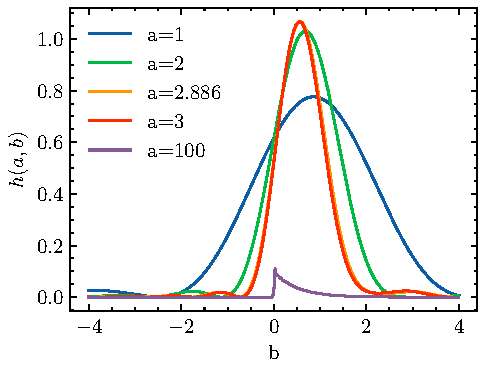
\includegraphics[width=\textwidth]{./img/bk-factor.pdf}
\end{subfigure}
\hspace{0.2cm}
\begin{subfigure}[b]{0.48\textwidth}
	\small
	% This file was created with tikzplotlib v0.10.1.
\begin{tikzpicture}

\definecolor{darkgray176}{RGB}{176,176,176}

\begin{axis}[
colorbar,
colorbar style={ytick={0,0.2,0.4,0.6,0.8,1,1.2},yticklabels={
  \(\displaystyle {0.0}\),
  \(\displaystyle {0.2}\),
  \(\displaystyle {0.4}\),
  \(\displaystyle {0.6}\),
  \(\displaystyle {0.8}\),
  \(\displaystyle {1.0}\),
  \(\displaystyle {1.2}\)
},ylabel={}},
colormap={mymap}{[1pt]
 rgb(0pt)=(0.001462,0.000466,0.013866);
  rgb(1pt)=(0.002267,0.00127,0.01857);
  rgb(2pt)=(0.003299,0.002249,0.024239);
  rgb(3pt)=(0.004547,0.003392,0.030909);
  rgb(4pt)=(0.006006,0.004692,0.038558);
  rgb(5pt)=(0.007676,0.006136,0.046836);
  rgb(6pt)=(0.009561,0.007713,0.055143);
  rgb(7pt)=(0.011663,0.009417,0.06346);
  rgb(8pt)=(0.013995,0.011225,0.071862);
  rgb(9pt)=(0.016561,0.013136,0.080282);
  rgb(10pt)=(0.019373,0.015133,0.088767);
  rgb(11pt)=(0.022447,0.017199,0.097327);
  rgb(12pt)=(0.025793,0.019331,0.10593);
  rgb(13pt)=(0.029432,0.021503,0.114621);
  rgb(14pt)=(0.033385,0.023702,0.123397);
  rgb(15pt)=(0.037668,0.025921,0.132232);
  rgb(16pt)=(0.042253,0.028139,0.141141);
  rgb(17pt)=(0.046915,0.030324,0.150164);
  rgb(18pt)=(0.051644,0.032474,0.159254);
  rgb(19pt)=(0.056449,0.034569,0.168414);
  rgb(20pt)=(0.06134,0.03659,0.177642);
  rgb(21pt)=(0.066331,0.038504,0.186962);
  rgb(22pt)=(0.071429,0.040294,0.196354);
  rgb(23pt)=(0.076637,0.041905,0.205799);
  rgb(24pt)=(0.081962,0.043328,0.215289);
  rgb(25pt)=(0.087411,0.044556,0.224813);
  rgb(26pt)=(0.09299,0.045583,0.234358);
  rgb(27pt)=(0.098702,0.046402,0.243904);
  rgb(28pt)=(0.104551,0.047008,0.25343);
  rgb(29pt)=(0.110536,0.047399,0.262912);
  rgb(30pt)=(0.116656,0.047574,0.272321);
  rgb(31pt)=(0.122908,0.047536,0.281624);
  rgb(32pt)=(0.129285,0.047293,0.290788);
  rgb(33pt)=(0.135778,0.046856,0.299776);
  rgb(34pt)=(0.142378,0.046242,0.308553);
  rgb(35pt)=(0.149073,0.045468,0.317085);
  rgb(36pt)=(0.15585,0.044559,0.325338);
  rgb(37pt)=(0.162689,0.043554,0.333277);
  rgb(38pt)=(0.169575,0.042489,0.340874);
  rgb(39pt)=(0.176493,0.041402,0.348111);
  rgb(40pt)=(0.183429,0.040329,0.354971);
  rgb(41pt)=(0.190367,0.039309,0.361447);
  rgb(42pt)=(0.197297,0.0384,0.367535);
  rgb(43pt)=(0.204209,0.037632,0.373238);
  rgb(44pt)=(0.211095,0.03703,0.378563);
  rgb(45pt)=(0.217949,0.036615,0.383522);
  rgb(46pt)=(0.224763,0.036405,0.388129);
  rgb(47pt)=(0.231538,0.036405,0.3924);
  rgb(48pt)=(0.238273,0.036621,0.396353);
  rgb(49pt)=(0.244967,0.037055,0.400007);
  rgb(50pt)=(0.25162,0.037705,0.403378);
  rgb(51pt)=(0.258234,0.038571,0.406485);
  rgb(52pt)=(0.26481,0.039647,0.409345);
  rgb(53pt)=(0.271347,0.040922,0.411976);
  rgb(54pt)=(0.27785,0.042353,0.414392);
  rgb(55pt)=(0.284321,0.043933,0.416608);
  rgb(56pt)=(0.290763,0.045644,0.418637);
  rgb(57pt)=(0.297178,0.04747,0.420491);
  rgb(58pt)=(0.303568,0.049396,0.422182);
  rgb(59pt)=(0.309935,0.051407,0.423721);
  rgb(60pt)=(0.316282,0.05349,0.425116);
  rgb(61pt)=(0.32261,0.055634,0.426377);
  rgb(62pt)=(0.328921,0.057827,0.427511);
  rgb(63pt)=(0.335217,0.06006,0.428524);
  rgb(64pt)=(0.3415,0.062325,0.429425);
  rgb(65pt)=(0.347771,0.064616,0.430217);
  rgb(66pt)=(0.354032,0.066925,0.430906);
  rgb(67pt)=(0.360284,0.069247,0.431497);
  rgb(68pt)=(0.366529,0.071579,0.431994);
  rgb(69pt)=(0.372768,0.073915,0.4324);
  rgb(70pt)=(0.379001,0.076253,0.432719);
  rgb(71pt)=(0.385228,0.078591,0.432955);
  rgb(72pt)=(0.391453,0.080927,0.433109);
  rgb(73pt)=(0.397674,0.083257,0.433183);
  rgb(74pt)=(0.403894,0.08558,0.433179);
  rgb(75pt)=(0.410113,0.087896,0.433098);
  rgb(76pt)=(0.416331,0.090203,0.432943);
  rgb(77pt)=(0.422549,0.092501,0.432714);
  rgb(78pt)=(0.428768,0.09479,0.432412);
  rgb(79pt)=(0.434987,0.097069,0.432039);
  rgb(80pt)=(0.441207,0.099338,0.431594);
  rgb(81pt)=(0.447428,0.101597,0.43108);
  rgb(82pt)=(0.453651,0.103848,0.430498);
  rgb(83pt)=(0.459875,0.106089,0.429846);
  rgb(84pt)=(0.4661,0.108322,0.429125);
  rgb(85pt)=(0.472328,0.110547,0.428334);
  rgb(86pt)=(0.478558,0.112764,0.427475);
  rgb(87pt)=(0.484789,0.114974,0.426548);
  rgb(88pt)=(0.491022,0.117179,0.425552);
  rgb(89pt)=(0.497257,0.119379,0.424488);
  rgb(90pt)=(0.503493,0.121575,0.423356);
  rgb(91pt)=(0.50973,0.123769,0.422156);
  rgb(92pt)=(0.515967,0.12596,0.420887);
  rgb(93pt)=(0.522206,0.12815,0.419549);
  rgb(94pt)=(0.528444,0.130341,0.418142);
  rgb(95pt)=(0.534683,0.132534,0.416667);
  rgb(96pt)=(0.54092,0.134729,0.415123);
  rgb(97pt)=(0.547157,0.136929,0.413511);
  rgb(98pt)=(0.553392,0.139134,0.411829);
  rgb(99pt)=(0.559624,0.141346,0.410078);
  rgb(100pt)=(0.565854,0.143567,0.408258);
  rgb(101pt)=(0.572081,0.145797,0.406369);
  rgb(102pt)=(0.578304,0.148039,0.404411);
  rgb(103pt)=(0.584521,0.150294,0.402385);
  rgb(104pt)=(0.590734,0.152563,0.40029);
  rgb(105pt)=(0.59694,0.154848,0.398125);
  rgb(106pt)=(0.603139,0.157151,0.395891);
  rgb(107pt)=(0.60933,0.159474,0.393589);
  rgb(108pt)=(0.615513,0.161817,0.391219);
  rgb(109pt)=(0.621685,0.164184,0.388781);
  rgb(110pt)=(0.627847,0.166575,0.386276);
  rgb(111pt)=(0.633998,0.168992,0.383704);
  rgb(112pt)=(0.640135,0.171438,0.381065);
  rgb(113pt)=(0.64626,0.173914,0.378359);
  rgb(114pt)=(0.652369,0.176421,0.375586);
  rgb(115pt)=(0.658463,0.178962,0.372748);
  rgb(116pt)=(0.66454,0.181539,0.369846);
  rgb(117pt)=(0.670599,0.184153,0.366879);
  rgb(118pt)=(0.676638,0.186807,0.363849);
  rgb(119pt)=(0.682656,0.189501,0.360757);
  rgb(120pt)=(0.688653,0.192239,0.357603);
  rgb(121pt)=(0.694627,0.195021,0.354388);
  rgb(122pt)=(0.700576,0.197851,0.351113);
  rgb(123pt)=(0.7065,0.200728,0.347777);
  rgb(124pt)=(0.712396,0.203656,0.344383);
  rgb(125pt)=(0.718264,0.206636,0.340931);
  rgb(126pt)=(0.724103,0.20967,0.337424);
  rgb(127pt)=(0.729909,0.212759,0.333861);
  rgb(128pt)=(0.735683,0.215906,0.330245);
  rgb(129pt)=(0.741423,0.219112,0.326576);
  rgb(130pt)=(0.747127,0.222378,0.322856);
  rgb(131pt)=(0.752794,0.225706,0.319085);
  rgb(132pt)=(0.758422,0.229097,0.315266);
  rgb(133pt)=(0.76401,0.232554,0.311399);
  rgb(134pt)=(0.769556,0.236077,0.307485);
  rgb(135pt)=(0.775059,0.239667,0.303526);
  rgb(136pt)=(0.780517,0.243327,0.299523);
  rgb(137pt)=(0.785929,0.247056,0.295477);
  rgb(138pt)=(0.791293,0.250856,0.29139);
  rgb(139pt)=(0.796607,0.254728,0.287264);
  rgb(140pt)=(0.801871,0.258674,0.283099);
  rgb(141pt)=(0.807082,0.262692,0.278898);
  rgb(142pt)=(0.812239,0.266786,0.274661);
  rgb(143pt)=(0.817341,0.270954,0.27039);
  rgb(144pt)=(0.822386,0.275197,0.266085);
  rgb(145pt)=(0.827372,0.279517,0.26175);
  rgb(146pt)=(0.832299,0.283913,0.257383);
  rgb(147pt)=(0.837165,0.288385,0.252988);
  rgb(148pt)=(0.841969,0.292933,0.248564);
  rgb(149pt)=(0.846709,0.297559,0.244113);
  rgb(150pt)=(0.851384,0.30226,0.239636);
  rgb(151pt)=(0.855992,0.307038,0.235133);
  rgb(152pt)=(0.860533,0.311892,0.230606);
  rgb(153pt)=(0.865006,0.316822,0.226055);
  rgb(154pt)=(0.869409,0.321827,0.221482);
  rgb(155pt)=(0.873741,0.326906,0.216886);
  rgb(156pt)=(0.878001,0.33206,0.212268);
  rgb(157pt)=(0.882188,0.337287,0.207628);
  rgb(158pt)=(0.886302,0.342586,0.202968);
  rgb(159pt)=(0.890341,0.347957,0.198286);
  rgb(160pt)=(0.894305,0.353399,0.193584);
  rgb(161pt)=(0.898192,0.358911,0.18886);
  rgb(162pt)=(0.902003,0.364492,0.184116);
  rgb(163pt)=(0.905735,0.37014,0.17935);
  rgb(164pt)=(0.90939,0.375856,0.174563);
  rgb(165pt)=(0.912966,0.381636,0.169755);
  rgb(166pt)=(0.916462,0.387481,0.164924);
  rgb(167pt)=(0.919879,0.393389,0.16007);
  rgb(168pt)=(0.923215,0.399359,0.155193);
  rgb(169pt)=(0.92647,0.405389,0.150292);
  rgb(170pt)=(0.929644,0.411479,0.145367);
  rgb(171pt)=(0.932737,0.417627,0.140417);
  rgb(172pt)=(0.935747,0.423831,0.13544);
  rgb(173pt)=(0.938675,0.430091,0.130438);
  rgb(174pt)=(0.941521,0.436405,0.125409);
  rgb(175pt)=(0.944285,0.442772,0.120354);
  rgb(176pt)=(0.946965,0.449191,0.115272);
  rgb(177pt)=(0.949562,0.45566,0.110164);
  rgb(178pt)=(0.952075,0.462178,0.105031);
  rgb(179pt)=(0.954506,0.468744,0.099874);
  rgb(180pt)=(0.956852,0.475356,0.094695);
  rgb(181pt)=(0.959114,0.482014,0.089499);
  rgb(182pt)=(0.961293,0.488716,0.084289);
  rgb(183pt)=(0.963387,0.495462,0.079073);
  rgb(184pt)=(0.965397,0.502249,0.073859);
  rgb(185pt)=(0.967322,0.509078,0.068659);
  rgb(186pt)=(0.969163,0.515946,0.063488);
  rgb(187pt)=(0.970919,0.522853,0.058367);
  rgb(188pt)=(0.97259,0.529798,0.053324);
  rgb(189pt)=(0.974176,0.53678,0.048392);
  rgb(190pt)=(0.975677,0.543798,0.043618);
  rgb(191pt)=(0.977092,0.55085,0.03905);
  rgb(192pt)=(0.978422,0.557937,0.034931);
  rgb(193pt)=(0.979666,0.565057,0.031409);
  rgb(194pt)=(0.980824,0.572209,0.028508);
  rgb(195pt)=(0.981895,0.579392,0.02625);
  rgb(196pt)=(0.982881,0.586606,0.024661);
  rgb(197pt)=(0.983779,0.593849,0.02377);
  rgb(198pt)=(0.984591,0.601122,0.023606);
  rgb(199pt)=(0.985315,0.608422,0.024202);
  rgb(200pt)=(0.985952,0.61575,0.025592);
  rgb(201pt)=(0.986502,0.623105,0.027814);
  rgb(202pt)=(0.986964,0.630485,0.030908);
  rgb(203pt)=(0.987337,0.63789,0.034916);
  rgb(204pt)=(0.987622,0.64532,0.039886);
  rgb(205pt)=(0.987819,0.652773,0.045581);
  rgb(206pt)=(0.987926,0.66025,0.05175);
  rgb(207pt)=(0.987945,0.667748,0.058329);
  rgb(208pt)=(0.987874,0.675267,0.065257);
  rgb(209pt)=(0.987714,0.682807,0.072489);
  rgb(210pt)=(0.987464,0.690366,0.07999);
  rgb(211pt)=(0.987124,0.697944,0.087731);
  rgb(212pt)=(0.986694,0.70554,0.095694);
  rgb(213pt)=(0.986175,0.713153,0.103863);
  rgb(214pt)=(0.985566,0.720782,0.112229);
  rgb(215pt)=(0.984865,0.728427,0.120785);
  rgb(216pt)=(0.984075,0.736087,0.129527);
  rgb(217pt)=(0.983196,0.743758,0.138453);
  rgb(218pt)=(0.982228,0.751442,0.147565);
  rgb(219pt)=(0.981173,0.759135,0.156863);
  rgb(220pt)=(0.980032,0.766837,0.166353);
  rgb(221pt)=(0.978806,0.774545,0.176037);
  rgb(222pt)=(0.977497,0.782258,0.185923);
  rgb(223pt)=(0.976108,0.789974,0.196018);
  rgb(224pt)=(0.974638,0.797692,0.206332);
  rgb(225pt)=(0.973088,0.805409,0.216877);
  rgb(226pt)=(0.971468,0.813122,0.227658);
  rgb(227pt)=(0.969783,0.820825,0.238686);
  rgb(228pt)=(0.968041,0.828515,0.249972);
  rgb(229pt)=(0.966243,0.836191,0.261534);
  rgb(230pt)=(0.964394,0.843848,0.273391);
  rgb(231pt)=(0.962517,0.851476,0.285546);
  rgb(232pt)=(0.960626,0.859069,0.29801);
  rgb(233pt)=(0.95872,0.866624,0.31082);
  rgb(234pt)=(0.956834,0.874129,0.323974);
  rgb(235pt)=(0.954997,0.881569,0.337475);
  rgb(236pt)=(0.953215,0.888942,0.351369);
  rgb(237pt)=(0.951546,0.896226,0.365627);
  rgb(238pt)=(0.950018,0.903409,0.380271);
  rgb(239pt)=(0.948683,0.910473,0.395289);
  rgb(240pt)=(0.947594,0.917399,0.410665);
  rgb(241pt)=(0.946809,0.924168,0.426373);
  rgb(242pt)=(0.946392,0.930761,0.442367);
  rgb(243pt)=(0.946403,0.937159,0.458592);
  rgb(244pt)=(0.946903,0.943348,0.47497);
  rgb(245pt)=(0.947937,0.949318,0.491426);
  rgb(246pt)=(0.949545,0.955063,0.50786);
  rgb(247pt)=(0.95174,0.960587,0.524203);
  rgb(248pt)=(0.954529,0.965896,0.540361);
  rgb(249pt)=(0.957896,0.971003,0.556275);
  rgb(250pt)=(0.961812,0.975924,0.571925);
  rgb(251pt)=(0.966249,0.980678,0.587206);
  rgb(252pt)=(0.971162,0.985282,0.602154);
  rgb(253pt)=(0.976511,0.989753,0.61676);
  rgb(254pt)=(0.982257,0.994109,0.631017);
  rgb(255pt)=(0.988362,0.998364,0.644924)
},
point meta max=1.06749233213328,
point meta min=1.43780715113311e-12,
tick pos=both,
x grid style={darkgray176},
xlabel={\(\displaystyle a\)},
xmin=0.01, xmax=8,
xtick style={color=black},
xtick={0,2,4,6,8},
xticklabels={
  \(\displaystyle {0}\),
  \(\displaystyle {2}\),
  \(\displaystyle {4}\),
  \(\displaystyle {6}\),
  \(\displaystyle {8}\)
},
y grid style={darkgray176},
ylabel={\(\displaystyle b\)},
ymin=-4, ymax=4,
ytick style={color=black},
ytick={-4,-2,0,2,4},
yticklabels={
  \(\displaystyle {\ensuremath{-}4}\),
  \(\displaystyle {\ensuremath{-}2}\),
  \(\displaystyle {0}\),
  \(\displaystyle {2}\),
  \(\displaystyle {4}\)
}
]
\addplot graphics [includegraphics cmd=\pgfimage,xmin=0.01, xmax=8, ymin=-4, ymax=4] {bk-factor-cmap-001.png};
\end{axis}

\end{tikzpicture}

	%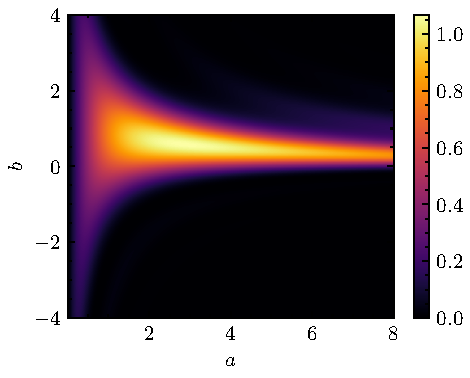
\includegraphics[width=\textwidth]{./img/bk-factor-cmap.pdf}
\end{subfigure}
\hspace{0.8cm}
\caption{Facteur de Boyd-Kleinman : \small dépendance en $b$ pour différentes valeurs de $a$ fixées et profil global}
\label{fig:bk-factor}
\end{figure}

Le profil de $h$ est tracé figure \ref{fig:bk-factor}. Le facteur de Boyd-Kleinman $h$ est maximal pour $a=2.8$ et $b=0.58$, et vaut alors $1.068$. On remarque également que le maximum est assez large en $a$ et se rétrécit en $b$ lorsqu'on se rapproche de la valeur optimale de $a$.

Physiquement, $a\gg1$ (\textit{i.e. $\zr \ll L$}) correspond à un faisceau fortement focalisé. L'intensité est alors importante au point focal, mais décroît rapidement dès que l'on s'en écarte. À l'inverse, $a\ll1$ (\textit{i.e. $\zr \gg L$}) correspond à un faisceau collimaté. L'intensité a alors un maximum moins intense mais est uniforme sur la longueur du cristal. Notons au passage que l'on retrouve bien dans cette limite le résultat pour les ondes planes donné par l'équation (\ref{eq:plane}), en considérant que $h(a,b) \approx a \sinc^2(ab)$ et $\P = \frac{\pi w_0^2}{2} I$.
L'optimum de $a$ correspond à un compromis entre ces deux cas limites, avec une longueur de Rayleigh comparable à la longueur du cristal.
% donnant $\alpha = \frac{\chie^2 \omega^2 L^2}{2 \varepsilon_0 c^3 \pi w_0^2 n_1^2 n_2}$ en passant des intensités aux puissances ($\P = \frac{\pi w_0^2}{2} I$). 

%et sera discuté plus bas en relation avec la réalisation expérimentale du doublage.

%On constate que l'optimum en $a$ est relativement souple, l'optimum $a=2.886$ et $a=3$ donnant essentiellement les mêmes courbes. 

\section{Réalisation de la génération  de seconde harmonique} 

Maintenant que l'on a discuté le principe de la génération de seconde harmonique et déterminé les valeurs optimales des paramètres $a$ et $b$, nous allons présenter la mise en place expérimentale du doublage dans cette section puis étudier les résultats obtenus à la lumière des calculs théoriques dans la section suivante. Tous les règlages sont d'abord faits à basse puissance (autour de $\SI{100}{mW}$) pour des raisons de sécurité ainsi que pour éviter d'endommager le cristal.

\subsection{Choix du cristal doubleur}

Le cristal doubleur choisi pour mon stage est un cristal de niobate de lithium périodiquement pôlé dopé au magnésium (Mgo\hc PPLN). Il présente l'avantage d'avoir un $\chi^{(2)}$ important selon l'axe extraordinaire et donc une bonne efficacité de conversion. En revanche, il présente des effets non-linéaires parasites conduisant notamment à des inhomogénéités d'indice optique et un couplage entre les faisceaux mais présente en revanche une dégradation optique plus importante. Il est donc avantageux lorsque l'on ne cherche pas à produire plus de 2 ou 3 watts de lumière verte, ce qui est notre cas. % En effet, %TODO

Le cristal commandé chez Covesion a une longueur $L=\SI{20}{mm}$ et présente 5 bandes avec des inversions de périodes différentes : $\Lambda = \qtylist[list-units = single]{6.83; 6.86 ; 6.90 ; 6.93 ; 6,96}{\micro\meter}$ (figure \ref{fig:sc}).

\subsection{Montage et alignement} 

\begin{figure}[htpb]
\centering
\hspace*{-0.8cm}
\begin{subfigure}[b]{0.48\textwidth}
	\centering
	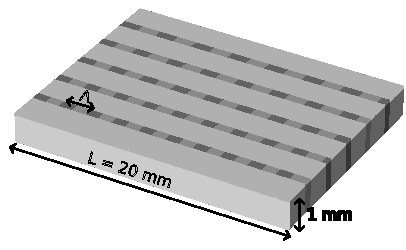
\includegraphics[height=5cm]{./img/cristal.pdf}
	\vspace{0.8cm}
	\caption{Schéma du cristal}
	\label{fig:sc}
\end{subfigure}
\centering
\hspace*{0.4cm}
\begin{subfigure}[b]{0.48\textwidth}
    % This file was created with tikzplotlib v0.10.1.
\begin{tikzpicture}

\definecolor{darkgray176}{RGB}{176,176,176}
\definecolor{limegreen018569}{RGB}{0,185,69}
\definecolor{teal1293165}{RGB}{12,93,165}

\begin{axis}[
legend cell align={left},
legend style={fill opacity=0.8, draw opacity=1, text opacity=1, draw=none},
tick pos=both,
x grid style={darkgray176},
xlabel={distance z à la lentille (\(\displaystyle \unit{cm}\))},
xmin=0, xmax=45,
xtick style={color=black},
xtick={0,10,20,30,40,50},
xticklabels={
  \(\displaystyle {0}\),
  \(\displaystyle {10}\),
  \(\displaystyle {20}\),
  \(\displaystyle {30}\),
  \(\displaystyle {40}\),
  \(\displaystyle {50}\)
},
y grid style={darkgray176},
ylabel={waist (\(\displaystyle \unit{\micro\meter}\))},
ymin=0, ymax=2750,
ytick style={color=black},
ytick={0,500,1000,1500,2000,2500},
yticklabels={
  \(\displaystyle {0}\),
  \(\displaystyle {500}\),
  \(\displaystyle {1000}\),
  \(\displaystyle {1500}\),
  \(\displaystyle {2000}\),
  \(\displaystyle {2500}\)
}
]
\path [draw=teal1293165, very thick]
(axis cs:41.9,1995)
--(axis cs:42.5,1995);

\path [draw=teal1293165, very thick]
(axis cs:27.4,1243)
--(axis cs:28,1243);

\path [draw=teal1293165, very thick]
(axis cs:5.9,100)
--(axis cs:6.5,100);

\path [draw=teal1293165, very thick]
(axis cs:4.4,68)
--(axis cs:5,68);

\path [draw=teal1293165, very thick]
(axis cs:10.1,301)
--(axis cs:10.7,301);

\path [draw=teal1293165, very thick]
(axis cs:3.9,87)
--(axis cs:4.5,87);

\path [draw=teal1293165, very thick]
(axis cs:14.9,535)
--(axis cs:15.5,535);

\path [draw=teal1293165, very thick]
(axis cs:27.9,1290)
--(axis cs:28.5,1290);

\path [draw=teal1293165, very thick]
(axis cs:20.9,910)
--(axis cs:21.5,910);

\path [draw=teal1293165, very thick]
(axis cs:42.2,1895)
--(axis cs:42.2,2095);

\path [draw=teal1293165, very thick]
(axis cs:27.7,1203)
--(axis cs:27.7,1283);

\path [draw=teal1293165, very thick]
(axis cs:6.2,60)
--(axis cs:6.2,140);

\path [draw=teal1293165, very thick]
(axis cs:4.7,28)
--(axis cs:4.7,108);

\path [draw=teal1293165, very thick]
(axis cs:10.4,261)
--(axis cs:10.4,341);

\path [draw=teal1293165, very thick]
(axis cs:4.2,47)
--(axis cs:4.2,127);

\path [draw=teal1293165, very thick]
(axis cs:15.2,495)
--(axis cs:15.2,575);

\path [draw=teal1293165, very thick]
(axis cs:28.2,1250)
--(axis cs:28.2,1330);

\path [draw=teal1293165, very thick]
(axis cs:21.2,870)
--(axis cs:21.2,950);

\addplot [very thick, limegreen018569, dashed]
table {%
0 270.726301163772
0.918367346938776 222.721199828545
1.83673469387755 175.632620773748
2.75510204081633 130.456828193017
3.6734693877551 90.1178810228514
4.59183673469388 64.4481408068083
5.51020408163265 71.5260452031186
6.42857142857143 104.921253075256
7.3469387755102 147.7533264157
8.26530612244898 193.865168357974
9.18367346938776 241.384430843346
10.1020408163265 289.619172915409
11.0204081632653 338.263461080832
11.9387755102041 387.162956389298
12.8571428571429 436.231844795124
13.7755102040816 485.418759363658
14.6938775510204 534.6911289581
15.6122448979592 584.027325342197
16.530612244898 633.412434375718
17.4489795918367 682.835843532488
18.3673469387755 732.289798043926
19.2857142857143 781.768501118613
20.2040816326531 831.267533516624
21.1224489795918 880.783467789853
22.0408163265306 930.313605135691
22.9591836734694 979.855791728942
23.8775510204082 1029.40828789381
24.7959183673469 1078.96967320668
25.7142857142857 1128.53877652943
26.6326530612245 1178.11462365802
27.5510204081633 1227.69639762392
28.469387755102 1277.28340822082
29.3877551020408 1326.87506835012
30.3061224489796 1376.47087547018
31.2244897959184 1426.07039690952
32.1428571428571 1475.6732581372
33.0612244897959 1525.27913331835
33.9795918367347 1574.88773765212
34.8979591836735 1624.49882111167
35.8163265306122 1674.1121632958
36.734693877551 1723.72756916869
37.6530612244898 1773.34486551404
38.5714285714286 1822.96389796764
39.4897959183673 1872.58452852128
40.4081632653061 1922.20663341293
41.3265306122449 1971.83010133522
42.2448979591837 2021.45483190749
43.1632653061224 2071.08073436749
44.0816326530612 2120.70772644647
45 2170.33573339861
};
\addlegendentry{$w_0 = \SI{62.6}{\micro\meter}$, $z_0 = \SI{4.9}{cm}$}
\addplot [very thick, teal1293165, mark=+, mark size=1.5, mark options={solid}, only marks]
table {%
42.2 1995
27.7 1243
6.2 100
4.7 68
10.4 301
4.2 87
15.2 535
28.2 1290
21.2 910
};
\addlegendentry{waist mesuré}
\end{axis}

\end{tikzpicture}

	\vspace{-0.5cm}
    \caption{Profil du faisceau incident sur le cristal}
    \label{fig:wincident}
\end{subfigure}
\caption{}
\end{figure}

Tout d'abord, on place une lentille devant le cristal afin d'obtenir un faisceau incident focalisé au centre du cristal et avec le bon souhaité (conformément à la valeur de $a$ voulue).

Les premières mesures ont été réalisées avec le faisceau issu de la fibre à cristaux photoniques et une lentille de focale $\SI{5}{cm}$, sachant que le faisceau incident sur la lentille est collimaté. Le profil du faisceau obtenu a été vérifié à la caméra en mesurant le waist à différentes positions (figure \ref{fig:wincident}). Avec le waist obtenu de $\SI{62.6}{\micro\meter}$, $a=\frac{L}{2\zr}=0.4$ ($\zr = \frac{n_1 \pi w_0^2}{\lambda_1} = \SI{2.4}{cm}$), 
 ce qui est suboptimal mais corresond à un pic en $b$ plus large et donc plus facile à trouver.

 Il s'agit ensuite d'optimiser la température du cristal (contrôlée à l'aide d'un four Covesion) et l'alignement du faisceau incident à l'aide des deux miroirs (cf. schéma figure \ref{fig:montage}). Pour estimer la température à laquelle se trouve l'optimum, on utilise une estimation des indices optiques $n_1$ et $n_2$ en fonction de la température à partir d'une équation dite de Sellmeier, pour laquelle on a pris les coefficients correspondants à un cristal de niobate de lithium congruent dopé à $\SI{5}{\percent}$ \cite{gayer,covesion}, et qui est tracée figure \ref{fig:sellmeier}. La température optimale calculée de la sorte est donnée figure \ref{fig:lp}.

\begin{figure}[htpb] 
\centering
\hspace*{-0.8cm}
\begin{subfigure}[h]{0.48\textwidth}
	\centering
	% This file was created with tikzplotlib v0.10.1.
\begin{tikzpicture}

\definecolor{darkgray176}{RGB}{176,176,176}
\definecolor{teal1293165}{RGB}{12,93,165}

\begin{axis}[
tick pos=both,
x grid style={darkgray176},
xlabel={T (°C)},
xmin=45, xmax=155,
xtick style={color=black},
xtick={40,60,80,100,120,140,160},
xticklabels={
  \(\displaystyle {40}\),
  \(\displaystyle {60}\),
  \(\displaystyle {80}\),
  \(\displaystyle {100}\),
  \(\displaystyle {120}\),
  \(\displaystyle {140}\),
  \(\displaystyle {160}\)
},
y grid style={darkgray176},
ylabel={\(\displaystyle n_2-n_1\) \(\displaystyle \left(\times 10^{-2}\right)\)},
ymin=7.6629850784832, ymax=7.89936722344637,
ytick style={color=black},
ytick={7.65,7.7,7.75,7.8,7.85,7.9},
yticklabels={
  \(\displaystyle {7.65}\),
  \(\displaystyle {7.70}\),
  \(\displaystyle {7.75}\),
  \(\displaystyle {7.80}\),
  \(\displaystyle {7.85}\),
  \(\displaystyle {7.90}\)
}
]
\addplot [very thick, teal1293165]
table {%
50 7.67372972143607
50.2004008016032 7.67410055301299
50.4008016032064 7.6744716219225
50.6012024048096 7.67484292818015
50.8016032064128 7.67521447180144
51.002004008016 7.67558625280187
51.2024048096192 7.67595827119703
51.4028056112224 7.67633052700245
51.6032064128256 7.67670302023364
51.8036072144289 7.67707575090624
52.0040080160321 7.67744871903582
52.2044088176353 7.67782192463806
52.4048096192385 7.67819536772842
52.6052104208417 7.67856904832276
52.8056112224449 7.67894296643661
53.0060120240481 7.67931712208565
53.2064128256513 7.67969151528551
53.4068136272545 7.6800661460521
53.6072144288577 7.68044101440086
53.8076152304609 7.68081612034774
54.0080160320641 7.68119146390829
54.2084168336673 7.68156704509853
54.4088176352705 7.68194286393391
54.6092184368737 7.68231892043048
54.809619238477 7.68269521460399
55.0100200400802 7.68307174647016
55.2104208416834 7.68344851604494
55.4108216432866 7.68382552334415
55.6112224448898 7.68420276838357
55.811623246493 7.68458025117922
56.0120240480962 7.68495797174684
56.2124248496994 7.68533593010248
56.4128256513026 7.68571412626198
56.6132264529058 7.68609256024129
56.813627254509 7.68647123205644
57.0140280561122 7.68685014172328
57.2144288577154 7.68722928925785
57.4148296593186 7.68760867467617
57.6152304609218 7.68798829799429
57.8156312625251 7.68836815922813
58.0160320641283 7.68874825839378
58.2164328657315 7.68912859550737
58.4168336673347 7.68950917058491
58.6172344689379 7.68988998364253
58.8176352705411 7.69027103469626
59.0180360721443 7.69065232376223
59.2184368737475 7.69103385085668
59.4188376753507 7.69141561599564
59.6192384769539 7.69179761919534
59.8196392785571 7.69217986047197
60.0200400801603 7.6925623398417
60.2204408817635 7.6929450573207
60.4208416833667 7.69332801292535
60.6212424849699 7.69371120667177
60.8216432865731 7.69409463857613
61.0220440881764 7.69447830865491
61.2224448897796 7.69486221692426
61.4228456913828 7.69524636340053
61.623246492986 7.69563074810002
61.8236472945892 7.69601537103908
62.0240480961924 7.69640023223404
62.2244488977956 7.69678533170128
62.4248496993988 7.69717066945721
62.625250501002 7.69755624551811
62.8256513026052 7.69794205990051
63.0260521042084 7.69832811262079
63.2264529058116 7.69871440369543
63.4268537074148 7.69910093314077
63.627254509018 7.69948770097342
63.8276553106212 7.69987470720976
64.0280561122244 7.70026195186642
64.2284569138277 7.70064943495981
64.4288577154309 7.7010371565065
64.6292585170341 7.70142511652296
64.8296593186373 7.70181331502586
65.0300601202405 7.7022017520318
65.2304609218437 7.70259042755725
65.4308617234469 7.70297934161892
65.6312625250501 7.70336849423341
65.8316633266533 7.70375788541733
66.0320641282565 7.70414751518742
66.2324649298597 7.70453738356025
66.4328657314629 7.70492749055252
66.6332665330661 7.705317836181
66.8336673346693 7.70570842046241
67.0340681362725 7.70609924341339
67.2344689378758 7.70649030505077
67.434869739479 7.7068816053913
67.6352705410822 7.70727314445177
67.8356713426854 7.70766492224886
68.0360721442886 7.70805693879959
68.2364729458918 7.7084491941207
68.436873747495 7.70884168822894
68.6372745490982 7.70923442114126
68.8376753507014 7.70962739287455
69.0380761523046 7.71002060344563
69.2384769539078 7.71041405287143
69.438877755511 7.7108077411689
69.6392785571142 7.71120166835497
69.8396793587174 7.71159583444665
70.0400801603206 7.71199023946076
70.2404809619239 7.71238488341437
70.4408817635271 7.71277976632447
70.6412825651303 7.71317488820813
70.8416833667335 7.7135702490823
71.0420841683367 7.71396584896404
71.2424849699399 7.71436168787045
71.4428857715431 7.71475776581863
71.6432865731463 7.71515408282561
71.8436873747495 7.71555063890847
72.0440881763527 7.71594743408444
72.2444889779559 7.71634446837064
72.4448897795591 7.71674174178414
72.6452905811623 7.71713925434225
72.8456913827655 7.71753700606199
73.0460921843687 7.71793499696072
73.2464929859719 7.71833322705557
73.4468937875751 7.71873169636383
73.6472945891784 7.71913040490269
73.8476953907816 7.71952935268949
74.0480961923848 7.71992853974148
74.248496993988 7.72032796607598
74.4488977955912 7.72072763171026
74.6492985971944 7.72112753666163
74.8496993987976 7.72152768094752
75.0501002004008 7.72192806458527
75.250501002004 7.72232868759222
75.4509018036072 7.72272954998585
75.6513026052104 7.72313065178345
75.8517034068136 7.7235319930026
76.0521042084168 7.72393357366061
76.25250501002 7.72433539377495
76.4529058116233 7.7247374533632
76.6533066132264 7.7251397524428
76.8537074148297 7.72554229103117
77.0541082164329 7.72594506914595
77.2545090180361 7.72634808680457
77.4549098196393 7.72675134402476
77.6553106212425 7.72715484082389
77.8557114228457 7.72755857721967
78.0561122244489 7.72796255322974
78.2565130260521 7.72836676887159
78.4569138276553 7.72877122416298
78.6573146292585 7.7291759191215
78.8577154308617 7.72958085376474
79.0581162324649 7.72998602811055
79.2585170340681 7.73039144217651
79.4589178356713 7.73079709598039
79.6593186372746 7.73120298953991
79.8597194388778 7.73160912287287
80.060120240481 7.73201549599691
80.2605210420842 7.73242210892993
80.4609218436874 7.73282896168968
80.6613226452906 7.73323605429397
80.8617234468938 7.73364338676061
81.062124248497 7.7340509591076
81.2625250501002 7.73445877135255
81.4629258517034 7.73486682351359
81.6633266533066 7.73527511560843
81.8637274549098 7.73568364765498
82.064128256513 7.7360924196713
82.2645290581162 7.7365014316753
82.4649298597194 7.73691068368492
82.6653306613227 7.73732017571809
82.8657314629259 7.73772990779285
83.0661322645291 7.73813987992722
83.2665330661323 7.7385500921392
83.4669338677355 7.73896054444685
83.6673346693387 7.73937123686821
83.8677354709419 7.73978216942139
84.0681362725451 7.74019334212439
84.2685370741483 7.74060475499545
84.4689378757515 7.74101640805265
84.6693386773547 7.74142830131406
84.8697394789579 7.74184043479789
85.0701402805611 7.74225280852239
85.2705410821643 7.74266542250563
85.4709418837675 7.74307827676584
85.6713426853707 7.74349137132133
85.8717434869739 7.74390470619015
86.0721442885772 7.74431828139082
86.2725450901804 7.74473209694144
86.4729458917836 7.74514615286028
86.6733466933868 7.74556044916581
86.87374749499 7.74597498587615
87.0741482965932 7.74638976300976
87.2745490981964 7.746804780585
87.4749498997996 7.74722003862016
87.6753507014028 7.74763553713371
87.875751503006 7.748051276144
88.0761523046092 7.74846725566953
88.2765531062124 7.74888347572871
88.4769539078156 7.7492999363399
88.6773547094188 7.74971663752173
88.877755511022 7.75013357929253
89.0781563126253 7.75055076167099
89.2785571142284 7.75096818467542
89.4789579158317 7.75138584832451
89.6793587174349 7.75180375263673
89.8797595190381 7.75222189763074
90.0801603206413 7.75264028332505
90.2805611222445 7.75305890973832
90.4809619238477 7.75347777688915
90.6813627254509 7.75389688479615
90.8817635270541 7.75431623347806
91.0821643286573 7.75473582295345
91.2825651302605 7.7551556532411
91.4829659318637 7.75557572435961
91.6833667334669 7.75599603632786
91.8837675350701 7.75641658916442
92.0841683366733 7.75683738288819
92.2845691382766 7.75725841751784
92.4849699398798 7.75767969307224
92.685370741483 7.75810120957012
92.8857715430862 7.75852296703032
93.0861723446894 7.75894496547176
93.2865731462926 7.75936720491321
93.4869739478958 7.75978968537361
93.687374749499 7.76021240687181
93.8877755511022 7.7606353694267
94.0881763527054 7.76105857305729
94.2885771543086 7.76148201778248
94.4889779559118 7.76190570362116
94.689378757515 7.76232963059238
94.8897795591182 7.76275379871523
95.0901803607214 7.76317820800849
95.2905811623247 7.76360285849131
95.4909819639279 7.76402775018279
95.6913827655311 7.76445288310188
95.8917835671343 7.76487825726782
96.0921843687375 7.76530387269951
96.2925851703407 7.7657297294162
96.4929859719439 7.76615582743698
96.6933867735471 7.76658216678099
96.8937875751503 7.76700874746736
97.0941883767535 7.76743556951534
97.2945891783567 7.76786263294413
97.4949899799599 7.76828993777285
97.6953907815631 7.76871748402086
97.8957915831663 7.76914527170729
98.0961923847695 7.76957330085151
98.2965931863727 7.77000157147278
98.496993987976 7.7704300835904
98.6973947895792 7.77085883722357
98.8977955911824 7.77128783239185
99.0981963927856 7.77171706911437
99.2985971943888 7.77214654741067
99.498997995992 7.77257626730008
99.6993987975952 7.77300622880199
99.8997995991984 7.77343643193578
100.100200400802 7.77386687672097
100.300601202405 7.77429756317698
100.501002004008 7.7747284913233
100.701402805611 7.77515966117939
100.901803607214 7.77559107276482
101.102204408818 7.77602272609901
101.302605210421 7.77645462120167
101.503006012024 7.77688675809221
101.703406813627 7.77731913679021
101.90380761523 7.77775175731539
102.104208416834 7.77818461968729
102.304609218437 7.7786177239255
102.50501002004 7.77905107004973
102.705410821643 7.77948465807961
102.905811623246 7.77991848803485
103.10621242485 7.78035255993514
103.306613226453 7.78078687380019
103.507014028056 7.78122142964977
103.707414829659 7.78165622750357
103.907815631263 7.78209126738134
104.108216432866 7.78252654930305
104.308617234469 7.78296207328824
104.509018036072 7.78339783935698
104.709418837675 7.78383384752894
104.909819639279 7.78427009782403
105.110220440882 7.78470659026214
105.310621242485 7.78514332486315
105.511022044088 7.78558030164702
105.711422845691 7.78601752063359
105.911823647295 7.78645498184289
106.112224448898 7.78689268529482
106.312625250501 7.7873306310094
106.513026052104 7.78776881900662
106.713426853707 7.78820724930642
106.913827655311 7.78864592192896
107.114228456914 7.78908483689422
107.314629258517 7.78952399422228
107.51503006012 7.7899633939333
107.715430861723 7.79040303604726
107.915831663327 7.79084292058432
108.11623246493 7.79128304756465
108.316633266533 7.79172341700844
108.517034068136 7.79216402893579
108.717434869739 7.79260488336693
108.917835671343 7.79304598032202
109.118236472946 7.79348731982141
109.318637274549 7.79392890188522
109.519038076152 7.79437072653382
109.719438877756 7.79481279378746
109.919839679359 7.79525510366632
110.120240480962 7.7956976561909
110.320641282565 7.79614045138142
110.521042084168 7.79658348925829
110.721442885772 7.79702676984186
110.921843687375 7.79747029315252
111.122244488978 7.79791405921069
111.322645290581 7.79835806803675
111.523046092184 7.79880231965118
111.723446893788 7.79924681407445
111.923847695391 7.79969155132703
112.124248496994 7.80013653142944
112.324649298597 7.8005817544021
112.5250501002 7.80102722026563
112.725450901804 7.80147292904059
112.925851703407 7.80191888074753
113.12625250501 7.80236507540706
113.326653306613 7.8028115130397
113.527054108216 7.80325819366618
113.72745490982 7.80370511730704
113.927855711423 7.80415228398303
114.128256513026 7.80459969371479
114.328657314629 7.80504734652294
114.529058116232 7.80549524242833
114.729458917836 7.80594338145164
114.929859719439 7.80639176361357
115.130260521042 7.80684038893495
115.330661322645 7.80728925743657
115.531062124248 7.80773836913915
115.731462925852 7.80818772406358
115.931863727455 7.80863732223067
116.132264529058 7.8090871636614
116.332665330661 7.80953724837641
116.533066132265 7.80998757639684
116.733466933868 7.81043814774347
116.933867735471 7.81088896243722
117.134268537074 7.81134002049915
117.334669338677 7.81179132195011
117.535070140281 7.81224286681104
117.735470941884 7.81269465510315
117.935871743487 7.81314668684736
118.13627254509 7.81359896206464
118.336673346693 7.81405148077616
118.537074148297 7.81450424300294
118.7374749499 7.81495724876602
118.937875751503 7.81541049808663
119.138276553106 7.81586399098586
119.338677354709 7.81631772748486
119.539078156313 7.8167717076048
119.739478957916 7.81722593136682
119.939879759519 7.8176803987922
120.140280561122 7.81813510990208
120.340681362725 7.81859006471786
120.541082164329 7.81904526326067
120.741482965932 7.8195007055518
120.941883767535 7.81995639161255
121.142284569138 7.82041232146424
121.342685370741 7.82086849512829
121.543086172345 7.82132491262599
121.743486973948 7.82178157397868
121.943887775551 7.82223847920775
122.144288577154 7.82269562833471
122.344689378758 7.8231530213809
122.545090180361 7.82361065836779
122.745490981964 7.82406853931681
122.945891783567 7.82452666424951
123.14629258517 7.82498503318734
123.346693386774 7.82544364615188
123.547094188377 7.82590250316457
123.74749498998 7.8263616042471
123.947895791583 7.826820949421
124.148296593186 7.8272805387078
124.34869739479 7.8277403721291
124.549098196393 7.82820044970669
124.749498997996 7.82866077146207
124.949899799599 7.829121337417
125.150300601202 7.82958214759315
125.350701402806 7.83004320201219
125.551102204409 7.83050450069585
125.751503006012 7.83096604366595
125.951903807615 7.83142783094419
126.152304609218 7.83188986255237
126.352705410822 7.83235213851228
126.553106212425 7.83281465884569
126.753507014028 7.83327742357462
126.953907815631 7.83374043272071
127.154308617234 7.83420368630603
127.354709418838 7.83466718435233
127.555110220441 7.83513092688159
127.755511022044 7.83559491391572
127.955911823647 7.83605914547669
128.156312625251 7.83652362158644
128.356713426854 7.836988342267
128.557114228457 7.8374533075404
128.75751503006 7.83791851742861
128.957915831663 7.83838397195376
129.158316633267 7.83884967113782
129.35871743487 7.83931561500291
129.559118236473 7.83978180357114
129.759519038076 7.84024823686464
129.959919839679 7.84071491490557
130.160320641283 7.84118183771603
130.360721442886 7.84164900531832
130.561122244489 7.84211641773451
130.761523046092 7.84258407498686
130.961923847695 7.8430519770976
131.162324649299 7.84352012408904
131.362725450902 7.84398851598342
131.563126252505 7.84445715280304
131.763527054108 7.84492603457019
131.963927855711 7.8453951613072
132.164328657315 7.84586453303655
132.364729458918 7.84633414978044
132.565130260521 7.84680401156126
132.765531062124 7.8472741184016
132.965931863727 7.84774447032373
133.166332665331 7.84821506735018
133.366733466934 7.84868590950336
133.567134268537 7.84915699680573
133.76753507014 7.84962832927989
133.967935871743 7.85009990694832
134.168336673347 7.85057172983361
134.36873747495 7.85104379795825
134.569138276553 7.85151611134483
134.769539078156 7.85198867001604
134.96993987976 7.85246147399441
135.170340681363 7.85293452330258
135.370741482966 7.85340781796324
135.571142284569 7.85388135799914
135.771543086172 7.85435514343287
135.971943887776 7.85482917428717
136.172344689379 7.85530345058478
136.372745490982 7.85577797234853
136.573146292585 7.85625273960115
136.773547094188 7.85672775236539
136.973947895792 7.85720301066415
137.174348697395 7.85767851452017
137.374749498998 7.85815426395637
137.575150300601 7.85863025899562
137.775551102204 7.8591064996608
137.975951903808 7.8595829859748
138.176352705411 7.86005971796064
138.376753507014 7.86053669564115
138.577154308617 7.86101391903942
138.77755511022 7.86149138817831
138.977955911824 7.86196910308092
139.178356713427 7.86244706377031
139.37875751503 7.86292527026942
139.579158316633 7.86340372260144
139.779559118236 7.86388242078941
139.97995991984 7.8643613648564
140.180360721443 7.86484055482561
140.380761523046 7.86531999072011
140.581162324649 7.86579967256311
140.781563126253 7.86627960037785
140.981963927856 7.8667597741874
141.182364729459 7.86724019401515
141.382765531062 7.86772085988421
141.583166332665 7.86820177181791
141.783567134269 7.86868292983955
141.983967935872 7.86916433397242
142.184368737475 7.86964598423983
142.384769539078 7.87012788066512
142.585170340681 7.87061002327167
142.785571142285 7.87109241208288
142.985971943888 7.8715750471221
143.186372745491 7.87205792841288
143.386773547094 7.87254105597852
143.587174348697 7.87302442984257
143.787575150301 7.87350805002847
143.987975951904 7.87399191655971
144.188376753507 7.87447602945988
144.38877755511 7.87496038875251
144.589178356713 7.87544499446113
144.789579158317 7.8759298466093
144.98997995992 7.87641494522076
145.190380761523 7.87690029031891
145.390781563126 7.87738588192761
145.591182364729 7.87787172007044
145.791583166333 7.87835780477102
145.991983967936 7.87884413605311
146.192384769539 7.87933071394047
146.392785571142 7.87981753845681
146.593186372745 7.88030460962585
146.793587174349 7.88079192747149
146.993987975952 7.88127949201733
147.194388777555 7.88176730328738
147.394789579158 7.88225536130547
147.595190380762 7.8827436660954
147.795591182365 7.88323221768104
147.995991983968 7.88372101608639
148.196392785571 7.88421006133526
148.396793587174 7.88469935345164
148.597194388778 7.88518889245959
148.797595190381 7.88567867838288
148.997995991984 7.88616871124574
149.198396793587 7.88665899107208
149.39879759519 7.88714951788596
149.599198396794 7.88764029171141
149.799599198397 7.88813131257258
150 7.8886225804935
};
\end{axis}

\end{tikzpicture}

	\caption{Différence d'indices optiques calculée par l'équation de Sellmeier}
	\label{fig:sellmeier}
\end{subfigure}
\centering
\hspace*{0.8cm}
\begin{subfigure}[h]{0.48\textwidth}
	% This file was created with tikzplotlib v0.10.1.
\begin{tikzpicture}

\definecolor{darkgray176}{RGB}{176,176,176}
\definecolor{teal1293165}{RGB}{12,93,165}

\begin{axis}[
tick pos=both,
x grid style={darkgray176},
xlabel={\(\displaystyle \Lambda\) à 20°C (\(\displaystyle \mu\)m)},
xmin=6.72052719717957, xmax=6.93925484373805,
xtick style={color=black},
xtick={6.7,6.75,6.8,6.85,6.9,6.95},
xticklabels={
  \(\displaystyle {6.70}\),
  \(\displaystyle {6.75}\),
  \(\displaystyle {6.80}\),
  \(\displaystyle {6.85}\),
  \(\displaystyle {6.90}\),
  \(\displaystyle {6.95}\)
},
y grid style={darkgray176},
ylabel={température optimale (°C)},
ymin=45, ymax=155,
ytick style={color=black},
ytick={40,60,80,100,120,140,160},
yticklabels={
  \(\displaystyle {40}\),
  \(\displaystyle {60}\),
  \(\displaystyle {80}\),
  \(\displaystyle {100}\),
  \(\displaystyle {120}\),
  \(\displaystyle {140}\),
  \(\displaystyle {160}\)
}
]
\addplot [very thick, teal1293165]
table {%
6.92931267798539 50
6.92895703234664 50.2004008016032
6.9286012069442 50.4008016032064
6.92824520182312 50.6012024048096
6.92788901702851 50.8016032064128
6.92753265260553 51.002004008016
6.92717610859925 51.2024048096192
6.92681938505485 51.4028056112224
6.92646248201755 51.6032064128256
6.92610539953248 51.8036072144289
6.92574813764485 52.0040080160321
6.9253906963998 52.2044088176353
6.92503307584272 52.4048096192385
6.92467527601864 52.6052104208417
6.92431729697291 52.8056112224449
6.92395913875081 53.0060120240481
6.92360080139765 53.2064128256513
6.92324228495854 53.4068136272545
6.92288358947903 53.6072144288577
6.92252471500425 53.8076152304609
6.92216566157971 54.0080160320641
6.92180642925051 54.2084168336673
6.9214470180623 54.4088176352705
6.92108742806025 54.6092184368737
6.92072765928977 54.809619238477
6.92036771179635 55.0100200400802
6.92000758562533 55.2104208416834
6.91964728082215 55.4108216432866
6.91928679743233 55.6112224448898
6.9189261355012 55.811623246493
6.91856529507438 56.0120240480962
6.91820427619722 56.2124248496994
6.9178430789153 56.4128256513026
6.91748170327411 56.6132264529058
6.91712014931913 56.813627254509
6.91675841709599 57.0140280561122
6.9163965066502 57.2144288577154
6.9160344180273 57.4148296593186
6.91567215127285 57.6152304609218
6.91530970643254 57.8156312625251
6.91494708355193 58.0160320641283
6.9145842826766 58.2164328657315
6.91422130385221 58.4168336673347
6.91385814712439 58.6172344689379
6.91349481253887 58.8176352705411
6.91313130014132 59.0180360721443
6.91276760997732 59.2184368737475
6.91240374209268 59.4188376753507
6.91203969653308 59.6192384769539
6.91167547334422 59.8196392785571
6.91131107257187 60.0200400801603
6.91094649426182 60.2204408817635
6.9105817384597 60.4208416833667
6.9102168052114 60.6212424849699
6.90985169456281 60.8216432865731
6.90948640655953 61.0220440881764
6.90912094124751 61.2224448897796
6.90875529867254 61.4228456913828
6.90838947888049 61.623246492986
6.90802348191721 61.8236472945892
6.90765730782858 62.0240480961924
6.90729095666047 62.2244488977956
6.90692442845876 62.4248496993988
6.90655772326947 62.625250501002
6.9061908411384 62.8256513026052
6.90582378211155 63.0260521042084
6.90545654623483 63.2264529058116
6.9050891335543 63.4268537074148
6.90472154411582 63.627254509018
6.90435377796547 63.8276553106212
6.90398583514917 64.0280561122244
6.90361771571299 64.2284569138277
6.90324941970295 64.4288577154309
6.90288094716515 64.6292585170341
6.90251229814557 64.8296593186373
6.90214347269025 65.0300601202405
6.90177447084537 65.2304609218437
6.90140529265695 65.4308617234469
6.90103593817112 65.6312625250501
6.90066640743401 65.8316633266533
6.9002967004917 66.0320641282565
6.89992681739041 66.2324649298597
6.8995567581763 66.4328657314629
6.89918652289545 66.6332665330661
6.89881611159409 66.8336673346693
6.89844552431846 67.0340681362725
6.89807476111471 67.2344689378758
6.89770382202907 67.434869739479
6.89733270710778 67.6352705410822
6.89696141639717 67.8356713426854
6.89658994994333 68.0360721442886
6.8962183077926 68.2364729458918
6.89584648999135 68.436873747495
6.89547449658578 68.6372745490982
6.89510232762221 68.8376753507014
6.89472998314701 69.0380761523046
6.89435746320649 69.2384769539078
6.89398476784697 69.438877755511
6.89361189711482 69.6392785571142
6.89323885105636 69.8396793587174
6.8928656297181 70.0400801603206
6.89249223314637 70.2404809619239
6.89211866138757 70.4408817635271
6.89174491448808 70.6412825651303
6.89137099249441 70.8416833667335
6.89099689545298 71.0420841683367
6.89062262341023 71.2424849699399
6.8902481764126 71.4428857715431
6.88987355450661 71.6432865731463
6.88949875773882 71.8436873747495
6.88912378615562 72.0440881763527
6.88874863980355 72.2444889779559
6.88837331872921 72.4448897795591
6.88799782297903 72.6452905811623
6.88762215259972 72.8456913827655
6.8872463076377 73.0460921843687
6.88687028813962 73.2464929859719
6.88649409415204 73.4468937875751
6.88611772572162 73.6472945891784
6.88574118289489 73.8476953907816
6.88536446571852 74.0480961923848
6.88498757423914 74.248496993988
6.88461050850343 74.4488977955912
6.88423326855806 74.6492985971944
6.88385585444966 74.8496993987976
6.88347826622491 75.0501002004008
6.88310050393056 75.250501002004
6.88272256761324 75.4509018036072
6.88234445731978 75.6513026052104
6.88196617309678 75.8517034068136
6.8815877149911 76.0521042084168
6.88120908304949 76.25250501002
6.88083027731863 76.4529058116233
6.88045129784534 76.6533066132264
6.88007214467649 76.8537074148297
6.8796928178588 77.0541082164329
6.87931331743916 77.2545090180361
6.87893364346424 77.4549098196393
6.87855379598108 77.6553106212425
6.87817377503641 77.8557114228457
6.87779358067707 78.0561122244489
6.87741321295004 78.2565130260521
6.87703267190209 78.4569138276553
6.87665195758018 78.6573146292585
6.87627107003129 78.8577154308617
6.8758900093022 79.0581162324649
6.87550877543994 79.2585170340681
6.8751273684914 79.4589178356713
6.87474578850356 79.6593186372746
6.87436403552333 79.8597194388778
6.87398210959781 80.060120240481
6.87360001077388 80.2605210420842
6.87321773909858 80.4609218436874
6.87283529461892 80.6613226452906
6.87245267738195 80.8617234468938
6.87206988743458 81.062124248497
6.87168692482405 81.2625250501002
6.87130378959722 81.4629258517034
6.87092048180131 81.6633266533066
6.87053700148341 81.8637274549098
6.87015334869048 82.064128256513
6.86976952346967 82.2645290581162
6.86938552586811 82.4649298597194
6.86900135593295 82.6653306613227
6.8686170137113 82.8657314629259
6.86823249925029 83.0661322645291
6.8678478125971 83.2665330661323
6.86746295379888 83.4669338677355
6.86707792290284 83.6673346693387
6.86669271995613 83.8677354709419
6.86630734500604 84.0681362725451
6.86592179809966 84.2685370741483
6.86553607928427 84.4689378757515
6.86515018860714 84.6693386773547
6.86476412611549 84.8697394789579
6.8643778918565 85.0701402805611
6.86399148587754 85.2705410821643
6.8636049082259 85.4709418837675
6.86321815894875 85.6713426853707
6.86283123809359 85.8717434869739
6.86244414570749 86.0721442885772
6.86205688183791 86.2725450901804
6.86166944653223 86.4729458917836
6.86128183983762 86.6733466933868
6.86089406180163 86.87374749499
6.86050611247151 87.0741482965932
6.86011799189465 87.2745490981964
6.85972970011849 87.4749498997996
6.85934123719037 87.6753507014028
6.85895260315774 87.875751503006
6.85856379806794 88.0761523046092
6.85817482196845 88.2765531062124
6.85778567490677 88.4769539078156
6.85739635693023 88.6773547094188
6.85700686808643 88.877755511022
6.85661720842266 89.0781563126253
6.85622737798662 89.2785571142284
6.85583737682564 89.4789579158317
6.85544720498732 89.6793587174349
6.85505686251909 89.8797595190381
6.85466634946855 90.0801603206413
6.85427566588318 90.2805611222445
6.85388481181054 90.4809619238477
6.85349378729822 90.6813627254509
6.85310259239371 90.8817635270541
6.85271122714469 91.0821643286573
6.85231969159866 91.2825651302605
6.8519279858033 91.4829659318637
6.85153610980608 91.6833667334669
6.85114406365479 91.8837675350701
6.85075184739691 92.0841683366733
6.85035946108019 92.2845691382766
6.84996690475219 92.4849699398798
6.84957417846065 92.685370741483
6.84918128225321 92.8857715430862
6.84878821617751 93.0861723446894
6.84839498028129 93.2865731462926
6.84800157461221 93.4869739478958
6.847607999218 93.687374749499
6.8472142541464 93.8877755511022
6.84682033944509 94.0881763527054
6.84642625516182 94.2885771543086
6.84603200134442 94.4889779559118
6.84563757804059 94.689378757515
6.84524298529799 94.8897795591182
6.84484822316462 95.0901803607214
6.84445329168817 95.2905811623247
6.84405819091638 95.4909819639279
6.84366292089717 95.6913827655311
6.84326748167821 95.8917835671343
6.8428718733075 96.0921843687375
6.84247609583277 96.2925851703407
6.8420801493019 96.4929859719439
6.84168403376276 96.6933867735471
6.84128774926325 96.8937875751503
6.84089129585119 97.0941883767535
6.84049467357446 97.2945891783567
6.84009788248105 97.4949899799599
6.83970092261876 97.6953907815631
6.8393037940356 97.8957915831663
6.83890649677943 98.0961923847695
6.83850903089819 98.2965931863727
6.83811139643985 98.496993987976
6.83771359345245 98.6973947895792
6.83731562198378 98.8977955911824
6.836917482082 99.0981963927856
6.83651917379495 99.2985971943888
6.83612069717068 99.498997995992
6.8357220522572 99.6993987975952
6.83532323910259 99.8997995991984
6.83492425775476 100.100200400802
6.83452510826181 100.300601202405
6.83412579067176 100.501002004008
6.8337263050327 100.701402805611
6.83332665139262 100.901803607214
6.8329268297997 101.102204408818
6.83252684030187 101.302605210421
6.83212668294736 101.503006012024
6.83172635778426 101.703406813627
6.83132586486057 101.90380761523
6.83092520422448 102.104208416834
6.83052437592416 102.304609218437
6.83012338000768 102.50501002004
6.82972221652322 102.705410821643
6.82932088551891 102.905811623246
6.82891938704293 103.10621242485
6.82851772114347 103.306613226453
6.82811588786868 103.507014028056
6.82771388726679 103.707414829659
6.82731171938604 103.907815631263
6.82690938427448 104.108216432866
6.82650688198056 104.308617234469
6.82610421255228 104.509018036072
6.82570137603804 104.709418837675
6.82529837248605 104.909819639279
6.82489520194454 105.110220440882
6.82449186446179 105.310621242485
6.82408836008604 105.511022044088
6.82368468886565 105.711422845691
6.82328085084883 105.911823647295
6.82287684608395 106.112224448898
6.82247267461928 106.312625250501
6.82206833650315 106.513026052104
6.82166383178396 106.713426853707
6.82125916050992 106.913827655311
6.82085432272946 107.114228456914
6.82044931849092 107.314629258517
6.82004414784259 107.51503006012
6.81963881083297 107.715430861723
6.8192333075104 107.915831663327
6.81882763792324 108.11623246493
6.81842180211986 108.316633266533
6.81801580014876 108.517034068136
6.8176096320583 108.717434869739
6.81720329789695 108.917835671343
6.81679679771305 109.118236472946
6.81639013155516 109.318637274549
6.81598329947163 109.519038076152
6.81557630151094 109.719438877756
6.81516913772168 109.919839679359
6.81476180815216 110.120240480962
6.81435431285099 110.320641282565
6.81394665186657 110.521042084168
6.81353882524747 110.721442885772
6.81313083304217 110.921843687375
6.8127226752992 111.122244488978
6.81231435206712 111.322645290581
6.81190586339443 111.523046092184
6.81149720932968 111.723446893788
6.81108838992142 111.923847695391
6.81067940521821 112.124248496994
6.81027025526868 112.324649298597
6.80986094012136 112.5250501002
6.80945145982482 112.725450901804
6.80904181442767 112.925851703407
6.8086320039785 113.12625250501
6.80822202852599 113.326653306613
6.80781188811867 113.527054108216
6.80740158280527 113.72745490982
6.80699111263434 113.927855711423
6.80658047765456 114.128256513026
6.80616967791464 114.328657314629
6.80575871346314 114.529058116232
6.80534758434876 114.729458917836
6.80493629062024 114.929859719439
6.8045248323262 115.130260521042
6.80411320951535 115.330661322645
6.80370142223644 115.531062124248
6.80328947053814 115.731462925852
6.80287735446918 115.931863727455
6.80246507407821 116.132264529058
6.80205262941415 116.332665330661
6.80164002052554 116.533066132265
6.80122724746124 116.733466933868
6.80081431027002 116.933867735471
6.80040120900057 117.134268537074
6.79998794370174 117.334669338677
6.79957451442238 117.535070140281
6.79916092121108 117.735470941884
6.79874716411674 117.935871743487
6.79833324318824 118.13627254509
6.79791915847428 118.336673346693
6.79750491002375 118.537074148297
6.79709049788551 118.7374749499
6.79667592210832 118.937875751503
6.79626118274105 119.138276553106
6.79584627983256 119.338677354709
6.7954312134317 119.539078156313
6.7950159835874 119.739478957916
6.79460059034846 119.939879759519
6.79418503376385 120.140280561122
6.79376931388232 120.340681362725
6.79335343075288 120.541082164329
6.79293738442444 120.741482965932
6.7925211749459 120.941883767535
6.79210480236619 121.142284569138
6.79168826673417 121.342685370741
6.79127156809883 121.543086172345
6.79085470650915 121.743486973948
6.79043768201407 121.943887775551
6.79002049466249 122.144288577154
6.78960314450342 122.344689378758
6.78918563158585 122.545090180361
6.78876795595877 122.745490981964
6.78835011767112 122.945891783567
6.78793211677195 123.14629258517
6.78751395331021 123.346693386774
6.78709562733499 123.547094188377
6.78667713889522 123.74749498998
6.78625848803995 123.947895791583
6.78583967481827 124.148296593186
6.78542069927925 124.34869739479
6.78500156147179 124.549098196393
6.78458226144508 124.749498997996
6.78416279924812 124.949899799599
6.78374317492998 125.150300601202
6.78332338853977 125.350701402806
6.7829034401266 125.551102204409
6.78248332973947 125.751503006012
6.78206305742755 125.951903807615
6.78164262323993 126.152304609218
6.78122202722573 126.352705410822
6.78080126943412 126.553106212425
6.78038034991406 126.753507014028
6.7799592687149 126.953907815631
6.7795380258856 127.154308617234
6.77911662147543 127.354709418838
6.77869505553349 127.555110220441
6.77827332810898 127.755511022044
6.77785143925105 127.955911823647
6.77742938900889 128.156312625251
6.77700717743167 128.356713426854
6.77658480456856 128.557114228457
6.77616227046879 128.75751503006
6.77573957518152 128.957915831663
6.77531671875602 129.158316633267
6.7748937012415 129.35871743487
6.77447052268716 129.559118236473
6.77404718314225 129.759519038076
6.77362368265598 129.959919839679
6.77320002127766 130.160320641283
6.77277619905642 130.360721442886
6.77235221604164 130.561122244489
6.77192807228255 130.761523046092
6.77150376782844 130.961923847695
6.77107930272853 131.162324649299
6.77065467703214 131.362725450902
6.77022989078857 131.563126252505
6.76980494404713 131.763527054108
6.76937983685712 131.963927855711
6.76895456926776 132.164328657315
6.7685291413285 132.364729458918
6.76810355308869 132.565130260521
6.76767780459748 132.765531062124
6.76725189590437 132.965931863727
6.7668258270586 133.166332665331
6.76639959810961 133.366733466934
6.76597320910677 133.567134268537
6.76554666009935 133.76753507014
6.76511995113678 133.967935871743
6.76469308226837 134.168336673347
6.7642660535436 134.36873747495
6.76383886501183 134.569138276553
6.76341151672239 134.769539078156
6.76298400872477 134.96993987976
6.76255634106836 135.170340681363
6.76212851380257 135.370741482966
6.76170052697675 135.571142284569
6.76127238064043 135.771543086172
6.76084407484302 135.971943887776
6.76041560963395 136.172344689379
6.75998698506263 136.372745490982
6.75955820117852 136.573146292585
6.75912925803115 136.773547094188
6.7587001556699 136.973947895792
6.75827089414431 137.174348697395
6.75784147350381 137.374749498998
6.7574118937979 137.575150300601
6.75698215507608 137.775551102204
6.75655225738784 137.975951903808
6.75612220078263 138.176352705411
6.75569198531006 138.376753507014
6.75526161101953 138.577154308617
6.75483107796068 138.77755511022
6.75440038618296 138.977955911824
6.75396953573589 139.178356713427
6.75353852666908 139.37875751503
6.75310735903197 139.579158316633
6.75267603287416 139.779559118236
6.75224454824525 139.97995991984
6.75181290519471 140.180360721443
6.75138110377221 140.380761523046
6.75094914402726 140.581162324649
6.75051702600941 140.781563126253
6.75008474976834 140.981963927856
6.74965231535353 141.182364729459
6.74921972281467 141.382765531062
6.74878697220132 141.583166332665
6.74835406356306 141.783567134269
6.74792099694954 141.983967935872
6.74748777241037 142.184368737475
6.74705438999519 142.384769539078
6.74662084975362 142.585170340681
6.74618715173528 142.785571142285
6.74575329598985 142.985971943888
6.74531928256688 143.186372745491
6.74488511151614 143.386773547094
6.74445078288722 143.587174348697
6.74401629672982 143.787575150301
6.74358165309362 143.987975951904
6.74314685202824 144.188376753507
6.74271189358338 144.38877755511
6.74227677780872 144.589178356713
6.74184150475402 144.789579158317
6.74140607446883 144.98997995992
6.74097048700304 145.190380761523
6.74053474240619 145.390781563126
6.74009884072806 145.591182364729
6.73966278201842 145.791583166333
6.73922656632693 145.991983967936
6.73879019370332 146.192384769539
6.73835366419732 146.392785571142
6.73791697785872 146.593186372745
6.73748013473718 146.793587174349
6.7370431348826 146.993987975952
6.73660597834459 147.194388777555
6.73616866517292 147.394789579158
6.73573119541741 147.595190380762
6.73529356912785 147.795591182365
6.73485578635391 147.995991983968
6.73441784714549 148.196392785571
6.73397975155234 148.396793587174
6.73354149962416 148.597194388778
6.73310309141093 148.797595190381
6.73266452696226 148.997995991984
6.73222580632807 149.198396793587
6.73178692955814 149.39879759519
6.73134789670233 149.599198396794
6.73090870781039 149.799599198397
6.73046936293223 150
};
\end{axis}

\end{tikzpicture}

	\caption{Température optimale calculée, en fonction de la période d'inversion $\Lambda$}
    \label{fig:lp}
\end{subfigure}
\caption{}
\end{figure}


%On peut estimer la valeur de la température à laquelle il faut se placer à partir d'une équation dite de Sellmeier donnant la dépendance en température et en longueur d'onde des indices optiques, pour laquelle on a pris les coefficients correspondants à un cristal de niobate de lithium congruent dopé à $\SI{5}{\percent}$ \cite{gayer,covesion}. La relation entre période d'inversion $\Lambda$ et température optimale calculée est donnée figure \ref{fig:lp}.

\begin{figure}[h]
	\centering
	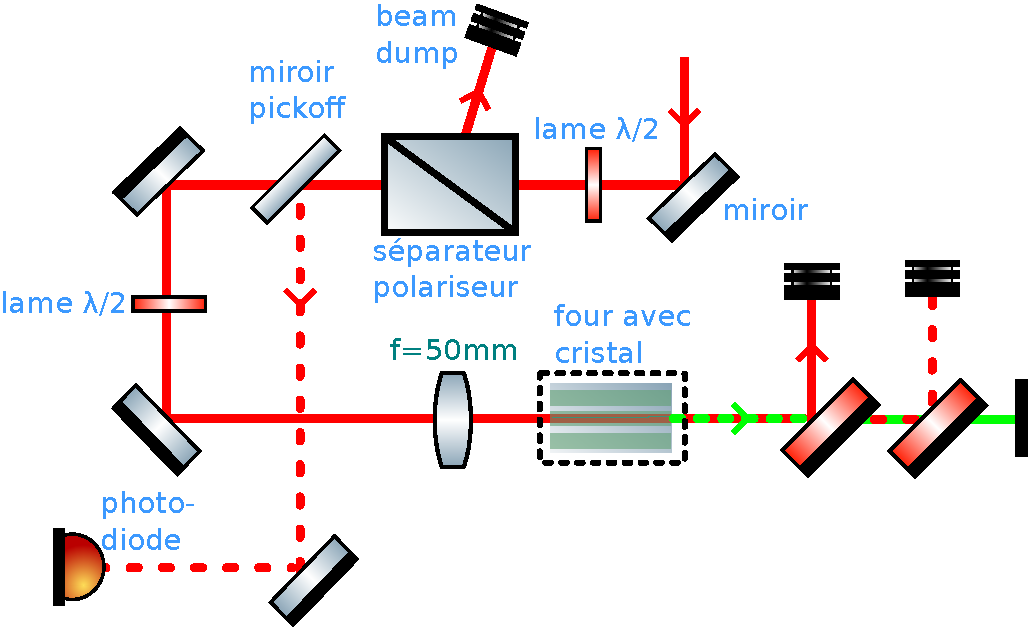
\includegraphics[height=8cm]{./img/schema.pdf}
	%%LaTeX with PSTricks extensions
%%Creator: Inkscape 1.2.2 (b0a8486, 2022-12-01)
%%Please note this file requires PSTricks extensions
\psset{xunit=.5pt,yunit=.5pt,runit=.5pt}
\begin{pspicture}(793.7007874,1122.51968504)
{
\newrgbcolor{curcolor}{0 0 0}
\pscustom[linewidth=0,linecolor=curcolor]
{
\newpath
\moveto(481.04617256,824.42653456)
\lineto(409.7164014,824.42653456)
\lineto(409.7164014,780.34567284)
\lineto(481.04617256,780.34567284)
\lineto(486.88963919,780.34567284)
\lineto(486.88963919,824.42653456)
\closepath
}
}
{
\newrgbcolor{curcolor}{1 0 0}
\pscustom[linewidth=5.15486004,linecolor=curcolor,linestyle=dashed,dash=1.36389005 4.09168005]
{
\newpath
\moveto(120.0614022,706.45175433)
\lineto(244.45846677,706.45175433)
}
}
{
\newrgbcolor{curcolor}{1 0 0}
\pscustom[linewidth=5.15486004,linecolor=curcolor]
{
\newpath
\moveto(494.93446299,1043.52720756)
\lineto(494.93446299,1097.75182413)
}
}
{
\newrgbcolor{curcolor}{1 0 0}
\pscustom[linewidth=5.15486004,linecolor=curcolor]
{
\newpath
\moveto(495.47285669,1030.41186898)
\lineto(495.47285669,951.80242016)
}
}
{
\newrgbcolor{curcolor}{1 0 0}
\pscustom[linewidth=5.15486004,linecolor=curcolor]
{
\newpath
\moveto(577.10211024,877.6012989)
\lineto(577.10211024,798.99183496)
}
}
{
\newrgbcolor{curcolor}{1 0 0}
\pscustom[linewidth=5.15486004,linecolor=curcolor,linestyle=dashed,dash=1.36389005 4.09168005]
{
\newpath
\moveto(654.13107402,879.39494929)
\lineto(654.13107402,800.78548535)
}
}
{
\newrgbcolor{curcolor}{1 0 0}
\pscustom[linewidth=5.15486004,linecolor=curcolor,linestyle=dashed,dash=1.36389005 4.09168005]
{
\newpath
\moveto(249.46311307,957.86754142)
\lineto(249.46311307,701.73977953)
}
}
{
\newrgbcolor{curcolor}{0 1 0}
\pscustom[linestyle=none,fillstyle=solid,fillcolor=curcolor]
{
\newpath
\moveto(598.18045984,801.48394205)
\lineto(707.27142047,801.48394205)
}
}
{
\newrgbcolor{curcolor}{0 1 0.01176471}
\pscustom[linewidth=5.15486004,linecolor=curcolor]
{
\newpath
\moveto(598.18045984,801.48394205)
\lineto(707.27142047,801.48394205)
}
}
{
\newrgbcolor{curcolor}{1 0 0}
\pscustom[linewidth=5.15486004,linecolor=curcolor,linestyle=dashed,dash=1.36389005 4.09168005]
{
\newpath
\moveto(643.00195276,801.39240189)
\lineto(600.92840315,801.39240189)
}
}
{
\newrgbcolor{curcolor}{1 0 0}
\pscustom[linewidth=5.15486004,linecolor=curcolor]
{
\newpath
\moveto(167.86343433,951.39717921)
\lineto(491.17700787,951.39717921)
}
}
{
\newrgbcolor{curcolor}{1 0 0}
\pscustom[linewidth=5.15486004,linecolor=curcolor]
{
\newpath
\moveto(342.90952819,942.48478866)
\lineto(372.07640693,1038.48422173)
}
}
{
\newrgbcolor{curcolor}{1 0 0}
\pscustom[linewidth=5.15486004,linecolor=curcolor]
{
\newpath
\moveto(164.03092913,802.17283654)
\lineto(571.41807874,802.17283654)
}
}
{
\newrgbcolor{curcolor}{0 0 0}
\pscustom[linewidth=1.55582199,linecolor=curcolor]
{
\newpath
\moveto(271.56784252,726.71496664)
\lineto(285.88115782,711.91918516)
\lineto(244.98555611,669.64509467)
\lineto(230.67224081,684.44087615)
\closepath
}
}
{
\newrgbcolor{curcolor}{0 0 0}
\pscustom[linestyle=none,fillstyle=solid,fillcolor=curcolor]
{
\newpath
\moveto(281.78957867,716.14868125)
\lineto(285.88115851,711.91918445)
\lineto(244.9855568,669.64509396)
\lineto(240.89397696,673.87459076)
\closepath
}
}
{
\newrgbcolor{curcolor}{0 0 0}
\pscustom[linewidth=1.55582199,linecolor=curcolor]
{
\newpath
\moveto(281.78957867,716.14868125)
\lineto(285.88115851,711.91918445)
\lineto(244.9855568,669.64509396)
\lineto(240.89397696,673.87459076)
\closepath
}
}
{
\newrgbcolor{curcolor}{0 0 0}
\pscustom[linewidth=2.21295946,linecolor=curcolor]
{
\newpath
\moveto(462.71419231,1054.11663288)
\lineto(462.71419231,1037.11303217)
\lineto(528.52526228,1037.11303217)
\lineto(528.52526228,1054.11663288)
\closepath
}
}
{
\newrgbcolor{curcolor}{0 0 0}
\pscustom[linewidth=2.21295946,linecolor=curcolor]
{
\newpath
\moveto(470.93876255,1037.11003103)
\lineto(470.93876255,1020.10643032)
\lineto(520.30069481,1020.10643032)
\lineto(520.30069481,1037.11003103)
\closepath
}
}
{
\newrgbcolor{curcolor}{0 0 0}
\pscustom[linewidth=2.21295946,linecolor=curcolor]
{
\newpath
\moveto(487.39370542,1071.11723245)
\lineto(487.39370542,1054.11363174)
\lineto(503.84574778,1054.11363174)
\lineto(503.84574778,1071.11723245)
\closepath
}
}
{
\newrgbcolor{curcolor}{0 0 0}
\pscustom[linewidth=1.34271185,linecolor=curcolor]
{
\newpath
\moveto(265.02399753,983.17442162)
\lineto(274.76085509,973.43756406)
\lineto(228.48038354,927.15709251)
\lineto(218.74352598,936.89395007)
\closepath
}
}
{
\newrgbcolor{curcolor}{1 0 0}
\pscustom[linewidth=5.15486004,linecolor=curcolor]
{
\newpath
\moveto(164.31138898,948.39497575)
\lineto(164.31138898,804.04807559)
}
}
{
\newrgbcolor{curcolor}{0 0 0}
\pscustom[linewidth=1.55582199,linecolor=curcolor]
{
\newpath
\moveto(187.46274995,973.34351622)
\lineto(172.66696847,987.65683153)
\lineto(130.39287798,946.76122981)
\lineto(145.18865946,932.44791451)
\closepath
}
}
{
\newrgbcolor{curcolor}{0 0 0}
\pscustom[linestyle=none,fillstyle=solid,fillcolor=curcolor]
{
\newpath
\moveto(176.89646456,983.56525237)
\lineto(172.66696776,987.65683221)
\lineto(130.39287727,946.7612305)
\lineto(134.62237407,942.66965066)
\closepath
}
}
{
\newrgbcolor{curcolor}{0 0 0}
\pscustom[linewidth=1.55582199,linecolor=curcolor]
{
\newpath
\moveto(176.89646456,983.56525237)
\lineto(172.66696776,987.65683221)
\lineto(130.39287727,946.7612305)
\lineto(134.62237407,942.66965066)
\closepath
}
}
{
\newrgbcolor{curcolor}{0 0 0}
\pscustom[linewidth=1.55582199,linecolor=curcolor]
{
\newpath
\moveto(144.30504945,823.26191341)
\lineto(129.99173414,808.46613193)
\lineto(170.88733586,766.19204144)
\lineto(185.20065116,780.98782292)
\closepath
}
}
{
\newrgbcolor{curcolor}{0 0 0}
\pscustom[linestyle=none,fillstyle=solid,fillcolor=curcolor]
{
\newpath
\moveto(134.0833133,812.69562803)
\lineto(129.99173346,808.46613122)
\lineto(170.88733517,766.19204073)
\lineto(174.97891501,770.42153754)
\closepath
}
}
{
\newrgbcolor{curcolor}{0 0 0}
\pscustom[linewidth=1.55582199,linecolor=curcolor]
{
\newpath
\moveto(134.0833133,812.69562803)
\lineto(129.99173346,808.46613122)
\lineto(170.88733517,766.19204073)
\lineto(174.97891501,770.42153754)
\closepath
}
}
{
\newrgbcolor{curcolor}{0 0 0}
\pscustom[linewidth=1.55582199,linecolor=curcolor]
{
\newpath
\moveto(188.87357969,870.88278205)
\lineto(188.87357969,879.85068139)
\lineto(142.60304234,879.85068139)
\lineto(142.60304234,870.88278205)
\closepath
}
}
{
\newrgbcolor{curcolor}{0 0 0}
\pscustom[linewidth=2.00976889,linecolor=curcolor]
{
\newpath
\moveto(354.17527824,830.89080241)
\lineto(340.31857065,830.89080241)
\curveto(337.49873338,824.07767415)(335.66243356,813.24519556)(335.66243356,801.00528545)
\curveto(335.66243356,788.76537534)(337.49873338,777.93289675)(340.31857065,771.12240413)
\lineto(354.17527824,771.12240413)
\curveto(357.00056447,777.93289675)(358.83141533,788.76537534)(358.83141533,801.00528545)
\curveto(358.83141533,813.24519556)(356.99511551,824.07767415)(354.17527824,830.89080241)
\closepath
}
}
{
\newrgbcolor{curcolor}{0 0 0}
\pscustom[linewidth=3.80579535,linecolor=curcolor]
{
\newpath
\moveto(303.3273003,982.38098145)
\lineto(387.37600492,982.38098145)
\lineto(387.37600492,920.84456797)
\lineto(303.3273003,920.84456797)
\closepath
}
}
{
\newrgbcolor{curcolor}{0 0 0}
\pscustom[linewidth=3.818419,linecolor=curcolor]
{
\newpath
\moveto(303.25676865,982.44545764)
\lineto(387.68641194,920.77997643)
}
}
{
\newrgbcolor{curcolor}{0 0 0}
\pscustom[linewidth=0.77791099,linecolor=curcolor]
{
\newpath
\moveto(367.10854123,1064.35028585)
\lineto(360.3175804,1045.69227224)
\lineto(383.74570412,1037.1651325)
\lineto(390.53666495,1055.82314611)
\closepath
}
}
{
\newrgbcolor{curcolor}{0 0 0}
\pscustom[linestyle=none,fillstyle=solid,fillcolor=curcolor]
{
\newpath
\moveto(363.08266641,1066.55055969)
\lineto(362.18595113,1064.08685443)
\lineto(394.02627975,1052.49792248)
\lineto(394.92299502,1054.96162773)
\closepath
}
}
{
\newrgbcolor{curcolor}{0 0 0}
\pscustom[linewidth=1.03721466,linecolor=curcolor]
{
\newpath
\moveto(363.08266641,1066.55055969)
\lineto(362.18595113,1064.08685443)
\lineto(394.02627975,1052.49792248)
\lineto(394.92299502,1054.96162773)
\closepath
}
}
{
\newrgbcolor{curcolor}{0 0 0}
\pscustom[linestyle=none,fillstyle=solid,fillcolor=curcolor]
{
\newpath
\moveto(360.88972652,1060.52550616)
\lineto(359.5586102,1056.86829374)
\lineto(391.39893881,1045.27936179)
\lineto(392.73005513,1048.93657421)
\closepath
}
}
{
\newrgbcolor{curcolor}{0 0 0}
\pscustom[linewidth=1.03721466,linecolor=curcolor]
{
\newpath
\moveto(360.88972652,1060.52550616)
\lineto(359.5586102,1056.86829374)
\lineto(391.39893881,1045.27936179)
\lineto(392.73005513,1048.93657421)
\closepath
}
}
{
\newrgbcolor{curcolor}{0 0 0}
\pscustom[linestyle=none,fillstyle=solid,fillcolor=curcolor]
{
\newpath
\moveto(358.3004173,1053.41143677)
\lineto(355.64516299,1046.11618471)
\lineto(387.48549161,1034.52725276)
\lineto(390.14074591,1041.82250482)
\closepath
}
}
{
\newrgbcolor{curcolor}{0 0 0}
\pscustom[linewidth=1.03721466,linecolor=curcolor]
{
\newpath
\moveto(358.3004173,1053.41143677)
\lineto(355.64516299,1046.11618471)
\lineto(387.48549161,1034.52725276)
\lineto(390.14074591,1041.82250482)
\closepath
}
}
{
\newrgbcolor{curcolor}{0 0 0}
\pscustom[linewidth=1.55582199,linecolor=curcolor]
{
\newpath
\moveto(432.92965953,928.32353653)
\lineto(441.89755888,928.32353653)
\lineto(441.89755888,974.59407388)
\lineto(432.92965953,974.59407388)
\closepath
}
}
{
\newrgbcolor{curcolor}{0 0 0}
\pscustom[linewidth=1.55582199,linecolor=curcolor]
{
\newpath
\moveto(472.62369163,930.19138016)
\lineto(487.4194731,915.87806485)
\lineto(529.69356359,956.77366656)
\lineto(514.89778212,971.08698187)
\closepath
}
}
{
\newrgbcolor{curcolor}{0 0 0}
\pscustom[linestyle=none,fillstyle=solid,fillcolor=curcolor]
{
\newpath
\moveto(483.18997701,919.96964401)
\lineto(487.41947382,915.87806416)
\lineto(529.69356431,956.77366588)
\lineto(525.4640675,960.86524572)
\closepath
}
}
{
\newrgbcolor{curcolor}{0 0 0}
\pscustom[linewidth=1.55582199,linecolor=curcolor]
{
\newpath
\moveto(483.18997701,919.96964401)
\lineto(487.41947382,915.87806416)
\lineto(529.69356431,956.77366588)
\lineto(525.4640675,960.86524572)
\closepath
}
}
{
\newrgbcolor{curcolor}{0 0 0}
\pscustom[linewidth=1.72786126,linecolor=curcolor]
{
\newpath
\moveto(672.12706254,826.58292406)
\lineto(688.55892777,810.15105883)
\lineto(643.14118242,764.73331348)
\lineto(626.70931719,781.16517871)
\closepath
}
}
{
\newrgbcolor{curcolor}{0 0 0}
\pscustom[linestyle=none,fillstyle=solid,fillcolor=curcolor]
{
\newpath
\moveto(683.86174365,814.84824295)
\lineto(688.55892856,810.15105804)
\lineto(643.14118321,764.73331269)
\lineto(638.4439983,769.4304976)
\closepath
}
}
{
\newrgbcolor{curcolor}{0 0 0}
\pscustom[linewidth=1.72786126,linecolor=curcolor]
{
\newpath
\moveto(683.86174365,814.84824295)
\lineto(688.55892856,810.15105804)
\lineto(643.14118321,764.73331269)
\lineto(638.4439983,769.4304976)
\closepath
}
}
{
\newrgbcolor{curcolor}{0 0 0}
\pscustom[linestyle=none,fillstyle=solid,fillcolor=curcolor]
{
\newpath
\moveto(708.28488327,822.25878137)
\lineto(714.4281542,822.25878137)
\lineto(714.4281542,774.72147664)
\lineto(708.28488327,774.72147664)
\closepath
}
}
{
\newrgbcolor{curcolor}{0 0 0}
\pscustom[linewidth=1.59849069,linecolor=curcolor]
{
\newpath
\moveto(708.28488327,822.25878137)
\lineto(714.4281542,822.25878137)
\lineto(714.4281542,774.72147664)
\lineto(708.28488327,774.72147664)
\closepath
}
}
{
\newrgbcolor{curcolor}{0 0 0}
\pscustom[linewidth=0.77791103,linecolor=curcolor]
{
\newpath
\moveto(564.59961652,899.80578202)
\lineto(564.59961652,879.95033824)
\lineto(589.53130622,879.95033824)
\lineto(589.53130622,899.80578202)
\closepath
}
}
{
\newrgbcolor{curcolor}{0 0 0}
\pscustom[linestyle=none,fillstyle=solid,fillcolor=curcolor]
{
\newpath
\moveto(560.0639935,900.49643284)
\lineto(560.0639935,897.87461241)
\lineto(593.94776509,897.87461241)
\lineto(593.94776509,900.49643284)
\closepath
}
}
{
\newrgbcolor{curcolor}{0 0 0}
\pscustom[linewidth=1.0372147,linecolor=curcolor]
{
\newpath
\moveto(560.0639935,900.49643284)
\lineto(560.0639935,897.87461241)
\lineto(593.94776509,897.87461241)
\lineto(593.94776509,900.49643284)
\closepath
}
}
{
\newrgbcolor{curcolor}{0 0 0}
\pscustom[linestyle=none,fillstyle=solid,fillcolor=curcolor]
{
\newpath
\moveto(560.0639935,894.08470467)
\lineto(560.0639935,890.19278042)
\lineto(593.94776509,890.19278042)
\lineto(593.94776509,894.08470467)
\closepath
}
}
{
\newrgbcolor{curcolor}{0 0 0}
\pscustom[linewidth=1.0372147,linecolor=curcolor]
{
\newpath
\moveto(560.0639935,894.08470467)
\lineto(560.0639935,890.19278042)
\lineto(593.94776509,890.19278042)
\lineto(593.94776509,894.08470467)
\closepath
}
}
{
\newrgbcolor{curcolor}{0 0 0}
\pscustom[linestyle=none,fillstyle=solid,fillcolor=curcolor]
{
\newpath
\moveto(560.0639935,886.51406999)
\lineto(560.0639935,878.75062473)
\lineto(593.94776509,878.75062473)
\lineto(593.94776509,886.51406999)
\closepath
}
}
{
\newrgbcolor{curcolor}{0 0 0}
\pscustom[linewidth=1.0372147,linecolor=curcolor]
{
\newpath
\moveto(560.0639935,886.51406999)
\lineto(560.0639935,878.75062473)
\lineto(593.94776509,878.75062473)
\lineto(593.94776509,886.51406999)
\closepath
}
}
{
\newrgbcolor{curcolor}{0 0 0}
\pscustom[linewidth=0.77791103,linecolor=curcolor]
{
\newpath
\moveto(641.75171731,901.91199935)
\lineto(641.75171731,882.05655556)
\lineto(666.68340701,882.05655556)
\lineto(666.68340701,901.91199935)
\closepath
}
}
{
\newrgbcolor{curcolor}{0 0 0}
\pscustom[linestyle=none,fillstyle=solid,fillcolor=curcolor]
{
\newpath
\moveto(637.21609429,902.60265016)
\lineto(637.21609429,899.98082974)
\lineto(671.09986588,899.98082974)
\lineto(671.09986588,902.60265016)
\closepath
}
}
{
\newrgbcolor{curcolor}{0 0 0}
\pscustom[linewidth=1.0372147,linecolor=curcolor]
{
\newpath
\moveto(637.21609429,902.60265016)
\lineto(637.21609429,899.98082974)
\lineto(671.09986588,899.98082974)
\lineto(671.09986588,902.60265016)
\closepath
}
}
{
\newrgbcolor{curcolor}{0 0 0}
\pscustom[linestyle=none,fillstyle=solid,fillcolor=curcolor]
{
\newpath
\moveto(637.21609429,896.19092199)
\lineto(637.21609429,892.29899774)
\lineto(671.09986588,892.29899774)
\lineto(671.09986588,896.19092199)
\closepath
}
}
{
\newrgbcolor{curcolor}{0 0 0}
\pscustom[linewidth=1.0372147,linecolor=curcolor]
{
\newpath
\moveto(637.21609429,896.19092199)
\lineto(637.21609429,892.29899774)
\lineto(671.09986588,892.29899774)
\lineto(671.09986588,896.19092199)
\closepath
}
}
{
\newrgbcolor{curcolor}{0 0 0}
\pscustom[linestyle=none,fillstyle=solid,fillcolor=curcolor]
{
\newpath
\moveto(637.21609429,888.62028731)
\lineto(637.21609429,880.85684206)
\lineto(671.09986588,880.85684206)
\lineto(671.09986588,888.62028731)
\closepath
}
}
{
\newrgbcolor{curcolor}{0 0 0}
\pscustom[linewidth=1.0372147,linecolor=curcolor]
{
\newpath
\moveto(637.21609429,888.62028731)
\lineto(637.21609429,880.85684206)
\lineto(671.09986588,880.85684206)
\lineto(671.09986588,888.62028731)
\closepath
}
}
{
\newrgbcolor{curcolor}{0 0 0}
\pscustom[linewidth=1.55582199,linecolor=curcolor]
{
\newpath
\moveto(103.77247789,686.14119811)
\curveto(101.76071535,686.14119811)(99.82240459,686.45334513)(97.98815051,687.02069344)
\lineto(97.98815051,727.1147133)
\curveto(99.82240459,727.67995251)(101.76071535,727.99209953)(103.77247789,727.99209953)
\curveto(114.95143017,727.99209953)(124.01456323,718.62557969)(124.01456323,707.06770337)
\curveto(124.01456323,695.50982705)(114.95143017,686.14119811)(103.77247789,686.14119811)
\closepath
}
}
{
\newrgbcolor{curcolor}{0 0 0}
\pscustom[linestyle=none,fillstyle=solid,fillcolor=curcolor]
{
\newpath
\moveto(92.20586346,683.15260126)
\lineto(97.99019091,683.15260126)
\lineto(97.99019091,730.98280442)
\lineto(92.20586346,730.98280442)
\closepath
}
}
{
\newrgbcolor{curcolor}{0 0 0}
\pscustom[linewidth=1.55582199,linecolor=curcolor]
{
\newpath
\moveto(92.20586346,683.15260126)
\lineto(97.99019091,683.15260126)
\lineto(97.99019091,730.98280442)
\lineto(92.20586346,730.98280442)
\closepath
}
}
{
\newrgbcolor{curcolor}{0 0.50196081 0.50196081}
\pscustom[linestyle=none,fillstyle=solid,fillcolor=curcolor]
{
\newpath
\moveto(320.27327762,861.60655507)
\lineto(320.27327762,859.73852447)
\lineto(318.12443197,859.73852447)
\curveto(317.31861485,859.73852447)(316.75698473,859.57573314)(316.43954162,859.25015046)
\curveto(316.13023808,858.92456779)(315.97558631,858.33851897)(315.97558631,857.49200402)
\lineto(315.97558631,856.28327833)
\lineto(319.67501946,856.28327833)
\lineto(319.67501946,854.53734124)
\lineto(315.97558631,854.53734124)
\lineto(315.97558631,842.60880598)
\lineto(313.7168565,842.60880598)
\lineto(313.7168565,854.53734124)
\lineto(311.56801085,854.53734124)
\lineto(311.56801085,856.28327833)
\lineto(313.7168565,856.28327833)
\lineto(313.7168565,857.23560766)
\curveto(313.7168565,858.75770666)(314.07092766,859.86468776)(314.77906998,860.55655094)
\curveto(315.4872123,861.2565537)(316.61047253,861.60655507)(318.14885067,861.60655507)
\closepath
}
}
{
\newrgbcolor{curcolor}{0 0.50196081 0.50196081}
\pscustom[linestyle=none,fillstyle=solid,fillcolor=curcolor]
{
\newpath
\moveto(322.44654179,853.96350177)
\lineto(338.0989289,853.96350177)
\lineto(338.0989289,851.91233092)
\lineto(322.44654179,851.91233092)
\closepath
\moveto(322.44654179,848.98208684)
\lineto(338.0989289,848.98208684)
\lineto(338.0989289,846.90649729)
\lineto(322.44654179,846.90649729)
\closepath
}
}
{
\newrgbcolor{curcolor}{0 0.50196081 0.50196081}
\pscustom[linestyle=none,fillstyle=solid,fillcolor=curcolor]
{
\newpath
\moveto(343.44662412,860.837366)
\lineto(353.12863892,860.837366)
\lineto(353.12863892,858.76177645)
\lineto(345.70535393,858.76177645)
\lineto(345.70535393,854.29315423)
\curveto(346.06349487,854.41524774)(346.42163581,854.50478297)(346.77977675,854.56175994)
\curveto(347.1379177,854.62687647)(347.49605864,854.65943474)(347.85419958,854.65943474)
\curveto(349.8890913,854.65943474)(351.50072554,854.10187441)(352.68910231,852.98675375)
\curveto(353.87747907,851.87163309)(354.47166745,850.36174343)(354.47166745,848.45708478)
\curveto(354.47166745,846.49544916)(353.86119994,844.96928037)(352.64026491,843.87857841)
\curveto(351.41932987,842.79601602)(349.69781148,842.25473482)(347.47570972,842.25473482)
\curveto(346.71059044,842.25473482)(345.92919202,842.31985136)(345.13151446,842.45008443)
\curveto(344.34197647,842.5803175)(343.52395,842.7756671)(342.67743505,843.03613324)
\lineto(342.67743505,845.51463135)
\curveto(343.40999607,845.11579258)(344.16697579,844.81869839)(344.94837421,844.62334878)
\curveto(345.72977263,844.42799918)(346.55593866,844.33032437)(347.42687232,844.33032437)
\curveto(348.83501739,844.33032437)(349.95013805,844.70067467)(350.77223431,845.44137525)
\curveto(351.59433056,846.18207584)(352.00537869,847.18731235)(352.00537869,848.45708478)
\curveto(352.00537869,849.72685721)(351.59433056,850.73209372)(350.77223431,851.47279431)
\curveto(349.95013805,852.2134949)(348.83501739,852.58384519)(347.42687232,852.58384519)
\curveto(346.7675674,852.58384519)(346.10826249,852.51058909)(345.44895757,852.36407688)
\curveto(344.79779222,852.21756468)(344.13034774,851.98965681)(343.44662412,851.68035326)
\closepath
}
}
{
\newrgbcolor{curcolor}{0 0.50196081 0.50196081}
\pscustom[linestyle=none,fillstyle=solid,fillcolor=curcolor]
{
\newpath
\moveto(368.85428391,855.75827627)
\lineto(368.85428391,853.65826802)
\curveto(368.21939769,854.00826939)(367.58044169,854.26873553)(366.93741591,854.43966644)
\curveto(366.30252969,854.61873691)(365.65950391,854.70827214)(365.00833856,854.70827214)
\curveto(363.55135608,854.70827214)(362.41995629,854.24431683)(361.61413917,853.31640621)
\curveto(360.80832205,852.39663515)(360.40541349,851.10244402)(360.40541349,849.43383281)
\curveto(360.40541349,847.7652216)(360.80832205,846.46696068)(361.61413917,845.53905006)
\curveto(362.41995629,844.619279)(363.55135608,844.15939347)(365.00833856,844.15939347)
\curveto(365.65950391,844.15939347)(366.30252969,844.24485892)(366.93741591,844.41578983)
\curveto(367.58044169,844.5948603)(368.21939769,844.85939622)(368.85428391,845.2093976)
\lineto(368.85428391,843.13380804)
\curveto(368.22753726,842.84078364)(367.57637191,842.62101533)(366.90078786,842.47450313)
\curveto(366.23334337,842.32799092)(365.52113127,842.25473482)(364.76415155,842.25473482)
\curveto(362.70484113,842.25473482)(361.06878819,842.90183039)(359.85599272,844.19602152)
\curveto(358.64319726,845.49021265)(358.03679953,847.23614975)(358.03679953,849.43383281)
\curveto(358.03679953,851.66407413)(358.64726704,853.41815079)(359.86820207,854.69606279)
\curveto(361.09727667,855.97397479)(362.77809723,856.61293079)(364.91066375,856.61293079)
\curveto(365.60252694,856.61293079)(366.27811099,856.53967469)(366.93741591,856.39316249)
\curveto(367.59672082,856.25478985)(368.23567682,856.04316111)(368.85428391,855.75827627)
\closepath
}
}
{
\newrgbcolor{curcolor}{0 0.50196081 0.50196081}
\pscustom[linestyle=none,fillstyle=solid,fillcolor=curcolor]
{
\newpath
\moveto(383.40782903,853.65826802)
\curveto(383.96945914,854.66757431)(384.64097341,855.41234468)(385.42237183,855.89257912)
\curveto(386.20377025,856.37281357)(387.12354131,856.61293079)(388.181685,856.61293079)
\curveto(389.60610921,856.61293079)(390.70495073,856.11234743)(391.47820959,855.1111807)
\curveto(392.25146844,854.11815354)(392.63809787,852.70186891)(392.63809787,850.86232679)
\lineto(392.63809787,842.60880598)
\lineto(390.37936806,842.60880598)
\lineto(390.37936806,850.78907069)
\curveto(390.37936806,852.09954096)(390.1473904,853.0722192)(389.68343509,853.70710542)
\curveto(389.21947978,854.34199163)(388.51133746,854.65943474)(387.55900814,854.65943474)
\curveto(386.39505007,854.65943474)(385.47527902,854.27280532)(384.79969497,853.49954646)
\curveto(384.12411091,852.72628761)(383.78631889,851.6722137)(383.78631889,850.33732473)
\lineto(383.78631889,842.60880598)
\lineto(381.52758908,842.60880598)
\lineto(381.52758908,850.78907069)
\curveto(381.52758908,852.10768053)(381.29561142,853.08035877)(380.83165611,853.70710542)
\curveto(380.3677008,854.34199163)(379.65141891,854.65943474)(378.68281046,854.65943474)
\curveto(377.53513153,854.65943474)(376.62350004,854.26873553)(375.94791599,853.48733711)
\curveto(375.27233193,852.71407826)(374.93453991,851.66407413)(374.93453991,850.33732473)
\lineto(374.93453991,842.60880598)
\lineto(372.6758101,842.60880598)
\lineto(372.6758101,856.28327833)
\lineto(374.93453991,856.28327833)
\lineto(374.93453991,854.15885138)
\curveto(375.44733262,854.99722677)(376.06186992,855.61583385)(376.77815181,856.01467263)
\curveto(377.49443369,856.4135114)(378.34501843,856.61293079)(379.32990602,856.61293079)
\curveto(380.32293318,856.61293079)(381.16537835,856.36060422)(381.85724154,855.85595107)
\curveto(382.55724429,855.35129793)(383.07410679,854.61873691)(383.40782903,853.65826802)
\closepath
}
}
{
\newrgbcolor{curcolor}{0 0.50196081 0.50196081}
\pscustom[linestyle=none,fillstyle=solid,fillcolor=curcolor]
{
\newpath
\moveto(410.84288504,802.56537827)
\lineto(486.19653543,803.0067515)
}
}
{
\newrgbcolor{curcolor}{0.60000002 0.60000002 0.60000002}
\pscustom[linestyle=none,fillstyle=solid,fillcolor=curcolor]
{
\newpath
\moveto(482.16185197,802.00899402)
\lineto(414.66908976,802.00899402)
}
}
{
\newrgbcolor{curcolor}{0.3764706 0.62352943 0.4509804}
\pscustom[linewidth=9.41665469,linecolor=curcolor,strokeopacity=0.59946299]
{
\newpath
\moveto(482.16185197,802.00899402)
\lineto(414.66908976,802.00899402)
}
}
{
\newrgbcolor{curcolor}{0.60000002 0.60000002 0.60000002}
\pscustom[linestyle=none,fillstyle=solid,fillcolor=curcolor]
{
\newpath
\moveto(481.87101732,814.91112945)
\lineto(414.37829291,814.91112945)
}
}
{
\newrgbcolor{curcolor}{0.3764706 0.62352943 0.4509804}
\pscustom[linewidth=9.41665469,linecolor=curcolor,strokeopacity=0.59946299]
{
\newpath
\moveto(481.87101732,814.91112945)
\lineto(414.37829291,814.91112945)
}
}
{
\newrgbcolor{curcolor}{0.60000002 0.60000002 0.60000002}
\pscustom[linestyle=none,fillstyle=solid,fillcolor=curcolor]
{
\newpath
\moveto(482.1112063,787.65752315)
\lineto(414.61851969,787.65752315)
}
}
{
\newrgbcolor{curcolor}{0.3764706 0.62352943 0.4509804}
\pscustom[linewidth=9.41665469,linecolor=curcolor,strokeopacity=0.59946299]
{
\newpath
\moveto(482.1112063,787.65752315)
\lineto(414.61851969,787.65752315)
}
}
{
\newrgbcolor{curcolor}{0 1 0}
\pscustom[linestyle=none,fillstyle=solid,fillcolor=curcolor]
{
\newpath
\moveto(488.47181102,801.94171843)
\lineto(597.56277165,801.94171843)
}
}
{
\newrgbcolor{curcolor}{0 1 0.01176471}
\pscustom[linewidth=5.15486004,linecolor=curcolor,linestyle=dashed,dash=1.36389005 2.7277801]
{
\newpath
\moveto(488.47181102,801.94171843)
\lineto(597.56277165,801.94171843)
}
}
{
\newrgbcolor{curcolor}{0 0 0}
\pscustom[linewidth=3.38783617,linecolor=curcolor,linestyle=dashed,dash=0.89636499 1.79273999]
{
\newpath
\moveto(404.14821445,830.99617064)
\lineto(494.53787406,830.99617064)
\curveto(495.22933885,830.99617064)(495.78600546,830.43950404)(495.78600546,829.74803925)
\lineto(495.78600546,774.95494422)
\curveto(495.78600546,774.26347943)(495.22933885,773.70681282)(494.53787406,773.70681282)
\lineto(404.14821445,773.70681282)
\curveto(403.45674965,773.70681282)(402.90008305,774.26347943)(402.90008305,774.95494422)
\lineto(402.90008305,829.74803925)
\curveto(402.90008305,830.43950404)(403.45674965,830.99617064)(404.14821445,830.99617064)
\closepath
}
}
{
\newrgbcolor{curcolor}{0 0 0}
\pscustom[linewidth=1.72786126,linecolor=curcolor]
{
\newpath
\moveto(603.37042632,827.14380595)
\lineto(619.80229155,810.71194072)
\lineto(574.3845462,765.29419537)
\lineto(557.95268097,781.7260606)
\closepath
}
}
{
\newrgbcolor{curcolor}{0 0 0}
\pscustom[linestyle=none,fillstyle=solid,fillcolor=curcolor]
{
\newpath
\moveto(615.10510743,815.40912484)
\lineto(619.80229234,810.71193993)
\lineto(574.38454699,765.29419458)
\lineto(569.68736208,769.99137949)
\closepath
}
}
{
\newrgbcolor{curcolor}{0 0 0}
\pscustom[linewidth=1.72786126,linecolor=curcolor]
{
\newpath
\moveto(615.10510743,815.40912484)
\lineto(619.80229234,810.71193993)
\lineto(574.38454699,765.29419458)
\lineto(569.68736208,769.99137949)
\closepath
}
}
\end{pspicture}

	\caption{Schéma du montage}
	\label{fig:montage}
\end{figure}

De façon plus détaillée, l'ajustement se fait ensuite selon le protocole suivant :
\begin{enumerate}
	\item À l'aide des quatre vis des deux miroirs, on cherche à obtenir un faisceau le plus horizontal possible à la hauteur du cristal, d'abord sans puis avec lentille. La procédure est analogue à celle pour coupler la fibre.
	\item On place ensuite le cristal au point focal de la lentille et on le translate transversalement (à l'aide d'une platine de translation) jusqu'à faire passer le faisceau par la bande avec la période d'inversion choisie.
	\item On tourne la lame demi-onde devant le cristal afin d'aligner la direction de polarisation (linéaire) avec l'axe extraordinaire du cristal.
	\item On se place à une température élevée que l'on laisse décroître et on attend de voir apparaître le pic principal.
	\item Lorsque l'alignement n'est pas bon, le pic principal et les pics secondaires sont d'amplitudes comparables et il est difficile de trouver la température optimale. Il s'agit donc d'alterner optimisation de l'alignement et de la température.
	\item Une fois dépassé quelques dizaines de $\unit{\micro\watt}$ de vert, on peut passer d'une estimation de la puissance à l'\oe il à une mesure au puissance-mètre.
	\item On fait une dernière recherche fine d'optimum de température (en variant par pas de $\SI{0.2}{\celsius}$ sur une plage de $\SI{1}{\celsius}$).
	\item On optimise finement l'alignement. %On note que changer un seul angle influence très fortement la puissance de vert produite, mais que la variation de l'angle correspondant sur le deuxième miroir permet de retrouver une puissance optimale semblable. Il faut donc `beam-walker' considérablement afin de trouver le véritable optimum. De plus, il y a une certaine compensation entre alignement (et donc $\Lambda$ effective pour l'angle du faisceau) et température (et donc $\Delta k$, mais aussi $\Lambda$ à travers la dilatation thermique).
\end{enumerate}





% Il faut noter que en pratique, on commence par choisir un waist et donc fixer un $a$, et on cherche ensuite à optimiser $b$ en ajustant la température et l'alignement.



%\begin{figure}[h]
%    \centering
%    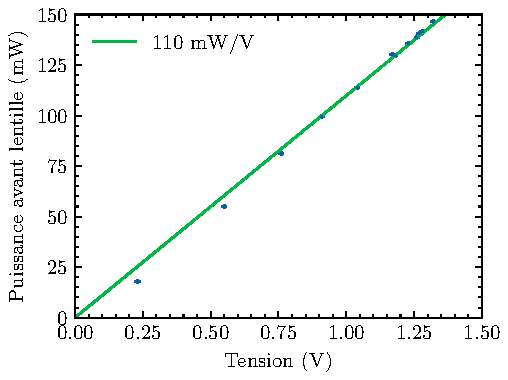
\includegraphics{../donnees/calib photodiode.pdf}
%    \caption{Calibration de la photodiode (après glan)}
%\end{figure}



Le régime de doublage trouvé initialement a été pour la bande avec $\Lambda = \SI{6.9}{\micro\meter}$ et une température optimale autour de $\SI{83}{\celsius}$.

\section{Étude à basse puissance}

L'étude du doublage est d'abord faite à basse puissance afin d'éviter les effets thermiques qui, comme nous le verrons, compliquent considérablement le comportement à haute puissance.

\subsection{Efficactité de conversion}

On vérifie tout d'abord que la puissance générée est bien quadratique en la puissance incidente, comme en témoignent les données présentées figure \ref{fig:quadra}. On fait ensuite varier la température autour de l'optimum, en gardant les autres paramètres fixés. On obtient alors les mesures figure \ref{fig:alphabp}, qui montrent un optimum à $\SI{83.3}{\celsius}$ (on rappelle que l'on travaille avec la bande $\Lambda = \SI{6.9}{\micro\meter}$). L'allure de la courbe est plutôt en accord avec celle prédite par la théorie de Boyd et Kleinman. 

\begin{figure}[htpb]
\centering
\hspace*{-0.4cm}
\begin{subfigure}[b]{0.45\textwidth}
    \centering
    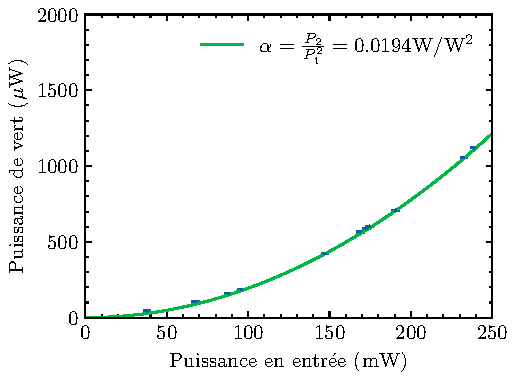
\includegraphics[height=6cm]{../donnees/conversion basse puissance 82.5 C.pdf}
    \caption{Vérification de la relation quadratique entre puissance incidente et doublée {(à~\SI{82.5}{\celsius})}}
    \label{fig:quadra}
\end{subfigure}
\hspace*{0.4cm}
\begin{subfigure}[b]{0.48\textwidth}
	\centering
	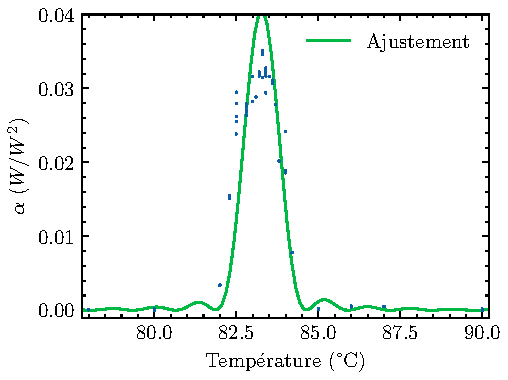
\includegraphics[height=6cm]{./img/alpha bp.pdf}
	\caption{Dépendance en température de l'efficacité de conversion}
	\label{fig:alphabp}
\end{subfigure}
\caption{Efficacité de conversion mesurée à basse puissance}
\end{figure}

En effet, le tracé de $\alpha$ en fonction de la température correspond, modulo la variation du préfacteur $\frac{\chie^2 L}{n_1 n_2}$, à la variation de $h(a,b)$ avec $a$ fixé et $b=-\Delta k_\mathsc{eff} \zr$ variant avec les indices optiques. Si on linéarise la variation d'indices optiques au voisinage de l'optimum de température, on a alors 
\begin{align}
	\delta b = - \zr \left[ 2\pi \left( \frac{\beta}{\Lambda} + \frac{1}{\lambda_2} \pdv{(n_2-n_1)}{T}  \right) + \frac{\dke}{n_1} \pdv{n_1}{T} \right] \delta T \approx -\left(0.3+5.5+\num{3e-4}\right) \delta T = - 5.8 \delta T
\end{align}
avec $\beta = \num{1.5e-5}$ le coefficient de dilatation thermique du cristal.
Les graphes de $\alpha(T)$ et de $h(a,b)$ à $a$ fixé (figure \ref{fig:bk-factor}) sont alors reliés par dilatation des deux axes.

L'accord quantitatif pose plus de difficultés. En effet, on ne peut se fier avec certitude ni à la valeur de température indiquée par le module de contrôle du four (dont la sonde est au niveau de la monture en cuivre et non à l'intérieur du cristal chauffé par le laser), qui indiquait d'ailleurs $\SI{30}{\celsius}$ laser et asservissement éteints dans une salle à $\SI{25}{\celsius}$, ni à la valeur exacte de la période d'inversion $\Lambda$ (qui varie d'ailleurs aussi avec la dilatation thermique). Il est donc difficile de se placer sur la courbe figure \ref{fig:lp}, or il est nécessaire de connaître la température du cristal au niveau du faisceau pour avoir une valeur exacte des indices optiques et de $\Lambda$ et ainsi pouvoir calculer $\dke$.
La valeur de $\chie$ varie d'un cristal à un autre et est également source d'incertitude. Covesion annonce d'ailleurs $\chie = \SI{28}{pm/V}$ alors que la valeur théorique correspondant à $\chi^{(2)}=\SI{50}{pm/V}$ est $\chie = \SI{32}{pm/V}$, ce qui fait passer le facteur devant $h$ de $\SI{5.5}{\percent\per\watt}$ à $\SI{4.2}{\percent\per\watt}$.

Encore une autre source d'incertitude est la détermination du waist du faisceau incident dont $\zr$ dépend quadratiquement. D'ailleurs, avec le waist déterminé à $\SI{62.6}{\micro\meter}$, $a=0.41$ ce qui correspond à un maximum de $h = 0.39$ et donc un maximum de seulement $\alphae{2.1}$ même pour $\chie = \SI{32}{pm/V}$. Il apparaît donc que $a$ a été sous-estimé et donc que le waist a été surestimé. Il faudrait plutôt $a=0.7$, ce qui correspond à un waist $\sqrt2$ fois plus petit, ce qui est difficiement reconciliable avec les mesures effectuées. % puisque un des waists $w(z)$ mesurés vaut $\SI{68\pm10}{\micro m}$, ce qui impose une borne supérieure sur la valeur de $w_0$. 
Il est également difficile d'imaginer un $\chie=\SI{40}{pm/V}$ qui permettrait d'augmenter suffisamment le préfacteur de $h$. Cette efficacité plus grande que prévu est d'autant plus étonnante que les mesures faites plus tard avec des longueurs de Rayleigh plus proches de l'optimum donnent toutes des efficacités plus faibles, et qui sont d'ailleurs en-dessous des valeurs théoriques (comme on pourrait s'y attendre au vu des imperfections inhérentes à la mise en pratique). Ces mesures sont récapitulées dans le tableau \ref{table:bp}. La seule différence au niveau de la mise en place est que la mesure dont il s'agit jusqu'à présent a été faite avec un faisceau sortant de la fibre à cristaux photoniques, alors que les mesures suivantes ont été faites avec un faisceau contournant la fibre (ce qui était nécessaire pour les tests à haute puissance).

\begin{table*}[h]\centering
\ra{1.3}
\begin{tabular}{@{}cccccc@{}}\toprule
	fibre & $w_0$ $(\unit{\micro\meter})$ & $zr$ $(\unit{cm})$ & $a$ & $\alpha$ théorique $(\unit{\percent\per\watt})$ & $\alpha$ mesuré $(\unit{\percent\per\watt})$ \\ \midrule
	oui & 63     & 2.5 & 0.4 & 1.6 & 3.5 \\ \midrule  
	non  & 30    & 0.6 & 1.7 & 4.15               & 2.8             \\
	non & 38    & 0.9 & 1.1 & 3.4                & 3.1             \\
	non & 64    & 2.6 & 0.4 & 1.6                & 1.2             \\ \bottomrule
\end{tabular}
\caption{}
\label{table:bp}
\end{table*}

Nonobstant ces difficultés, on peut également s'intéresser à la largeur à mi-hauteur (FWHM) de la courbe puisqu'il s'agit d'une quantité indépendante de la valeur du préfacteur.
La comparaison présente de nouveau quelques subtilités du fait de l'incertitude à la fois sur la température et sur la période d'inversion $\Lambda$. La méthode qui a été retenue est de fixer la valeur de $\Lambda$, ce qui fixe la température correspondant à l'optimum théorique.
On trouve figure \ref{fig:fwhm} le tracé de la largeur à mi-hauteur de $\alpha(T)$ en fonction de la longueur de Rayleigh $\zr$, pour différentes valeurs de $\Lambda$. Au cours de cette étude, il a été constaté numériquement que la largeur à mi-hauteur en b de $h$ vérifiait assez précisément une relation affine en $\frac1a$, soit une relation affine en $\zr$ (figure \ref{fig:baff}), ce qui permet de simplifier grandement les calculs.

D'après la courbe figure \ref{fig:fwhm}, on s'attend donc à une largeur $\delta T = \SI{1.2}{\celsius}$, ce qui est clairement inférieur à la largeur de la courbe expérimentale. Les longueurs de Rayleigh donnant une largeur semblable à celle observée expérimentalement sont inférieures à $\SI{0.2}{cm}$ et donc clairement irréalistes. L'étude de la largeur de la courbe ne permet donc malheureusement pas d'éclairer les choses. Comme notre objectif n'est pas de vérifier la théorie de Boyd-Kleinman à basse puissance mais d'obtenir quelques watts de lumière verte, nous n'avons pas poussé plus loin l'acquisition de données dans différentes configurations car cela est très chronophage au niveau de la recherche d'optimum et de l'attente de la thermalisation. En particulier, nous n'avons pas de mesures détaillées de la dépendance en température de l'efficacité dans les configurations correspondant aux valeurs présentées dans le tableau \ref{table:bp}.





%La largeur en température mesurée étant de $\SI{1.6}{\celsius}$, on voit que cela ne correspond pas au calculs pour $\zr=\SI{2.4}{cm}$, mais supposerait plutôt $\zr=\SI{0.5}{cm}$, ce qui n'est pas possible. Il est à l'inverse plus réaliste d'approcher les données par une courbe de largeur $\SI{1.2}{\celsius}$.

\begin{figure}[htpb] 
\centering
\hspace*{-0.8cm}
\begin{subfigure}[b]{0.48\textwidth}
	\small
	% This file was created with tikzplotlib v0.10.1.
\begin{tikzpicture}

\definecolor{darkgray176}{RGB}{176,176,176}
\definecolor{darkorange2551490}{RGB}{255,149,0}
\definecolor{limegreen018569}{RGB}{0,185,69}
\definecolor{teal1293165}{RGB}{12,93,165}

\begin{axis}[
legend cell align={left},
legend style={fill opacity=0.8, draw opacity=1, text opacity=1, draw=none},
tick pos=both,
x grid style={darkgray176},
xlabel={\(\displaystyle z_R\) ($\unit{cm}$)},
xmin=-0.045, xmax=3.145,
xtick style={color=black},
y grid style={darkgray176},
ylabel={\(\displaystyle \delta T\) FWHM ($\unit{celsius}$)},
ymin=0.971943887775549, ymax=1.63326653306614,
ytick style={color=black}
]
\addplot [teal1293165, mark=square*, mark size=1.5, mark options={solid}, only marks]
table {%
0.1 1.60320641282566
0.174358974358974 1.40280561122245
0.248717948717949 1.20240480961924
0.323076923076923 1.40280561122243
0.397435897435897 1.40280561122243
0.471794871794872 1.20240480961922
0.546153846153846 1.20240480961922
0.620512820512821 1.20240480961922
0.694871794871795 1.00200400801603
0.769230769230769 1.20240480961925
0.843589743589744 1.20240480961925
0.917948717948718 1.20240480961925
0.992307692307692 1.20240480961925
1.06666666666667 1.20240480961925
1.14102564102564 1.20240480961925
1.21538461538462 1.20240480961925
1.28974358974359 1.00200400801604
1.36410256410256 1.00200400801604
1.43846153846154 1.00200400801604
1.51282051282051 1.00200400801604
1.58717948717949 1.00200400801604
1.66153846153846 1.00200400801604
1.73589743589744 1.00200400801604
1.81025641025641 1.00200400801604
1.88461538461538 1.00200400801604
1.95897435897436 1.00200400801604
2.03333333333333 1.20240480961924
2.10769230769231 1.20240480961924
2.18205128205128 1.20240480961924
2.25641025641026 1.20240480961924
2.33076923076923 1.20240480961924
2.40512820512821 1.20240480961924
2.47948717948718 1.20240480961924
2.55384615384615 1.20240480961924
2.62820512820513 1.20240480961924
2.7025641025641 1.20240480961924
2.77692307692308 1.20240480961924
2.85128205128205 1.20240480961924
2.92564102564103 1.20240480961924
3 1.20240480961924
};
\addlegendentry{$\Lambda = 6.87$}
\addplot [limegreen018569, mark=*, mark size=1.5, mark options={solid}, only marks]
table {%
0.1 1.60320641282566
0.174358974358974 1.60320641282564
0.248717948717949 1.40280561122245
0.323076923076923 1.20240480961924
0.397435897435897 1.40280561122245
0.471794871794872 1.20240480961924
0.546153846153846 1.20240480961924
0.620512820512821 1.20240480961924
0.694871794871795 1.20240480961924
0.769230769230769 1.20240480961924
0.843589743589744 1.00200400801603
0.917948717948718 1.20240480961924
0.992307692307692 1.20240480961924
1.06666666666667 1.20240480961924
1.14102564102564 1.20240480961924
1.21538461538462 1.20240480961924
1.28974358974359 1.20240480961924
1.36410256410256 1.20240480961924
1.43846153846154 1.20240480961924
1.51282051282051 1.20240480961924
1.58717948717949 1.00200400801603
1.66153846153846 1.00200400801603
1.73589743589744 1.00200400801603
1.81025641025641 1.00200400801603
1.88461538461538 1.00200400801603
1.95897435897436 1.00200400801603
2.03333333333333 1.00200400801603
2.10769230769231 1.00200400801603
2.18205128205128 1.00200400801603
2.25641025641026 1.00200400801603
2.33076923076923 1.00200400801603
2.40512820512821 1.00200400801603
2.47948717948718 1.20240480961922
2.55384615384615 1.20240480961922
2.62820512820513 1.20240480961922
2.7025641025641 1.20240480961922
2.77692307692308 1.20240480961922
2.85128205128205 1.20240480961922
2.92564102564103 1.20240480961922
3 1.20240480961922
};
\addlegendentry{$\Lambda = 6.88$}
\addplot [darkorange2551490, mark=triangle*, mark size=1.5, mark options={solid}, only marks]
table {%
0.1 1.60320641282564
0.174358974358974 1.40280561122245
0.248717948717949 1.40280561122245
0.323076923076923 1.40280561122245
0.397435897435897 1.20240480961924
0.471794871794872 1.20240480961924
0.546153846153846 1.40280561122245
0.620512820512821 1.20240480961924
0.694871794871795 1.20240480961924
0.769230769230769 1.20240480961924
0.843589743589744 1.20240480961924
0.917948717948718 1.20240480961924
0.992307692307692 1.20240480961924
1.06666666666667 1.20240480961924
1.14102564102564 1.00200400801603
1.21538461538462 1.20240480961924
1.28974358974359 1.20240480961924
1.36410256410256 1.20240480961924
1.43846153846154 1.20240480961924
1.51282051282051 1.20240480961924
1.58717948717949 1.20240480961924
1.66153846153846 1.20240480961924
1.73589743589744 1.20240480961924
1.81025641025641 1.20240480961924
1.88461538461538 1.20240480961924
1.95897435897436 1.20240480961924
2.03333333333333 1.20240480961924
2.10769230769231 1.20240480961924
2.18205128205128 1.20240480961924
2.25641025641026 1.20240480961924
2.33076923076923 1.20240480961924
2.40512820512821 1.20240480961924
2.47948717948718 1.20240480961924
2.55384615384615 1.20240480961924
2.62820512820513 1.20240480961924
2.7025641025641 1.00200400801603
2.77692307692308 1.00200400801603
2.85128205128205 1.00200400801603
2.92564102564103 1.00200400801603
3 1.00200400801603
};
\addlegendentry{$\Lambda = 6.9$}
\end{axis}
\end{tikzpicture}

	\caption{$\delta T$ FWHM calculé}
	\label{fig:fwhm}
\end{subfigure}
\hspace{0.2cm}
\begin{subfigure}[b]{0.48\textwidth}
	\small
	% This file was created with tikzplotlib v0.10.1.
\begin{tikzpicture}

\definecolor{darkgray176}{RGB}{176,176,176}
\definecolor{limegreen018569}{RGB}{0,185,69}
\definecolor{teal1293165}{RGB}{12,93,165}

\begin{axis}[
legend cell align={left},
legend style={
  fill opacity=0.8,
  draw opacity=1,
  text opacity=1,
  at={(0.03,0.97)},
  anchor=north west,
  draw=none
},
tick pos=both,
x grid style={darkgray176},
xlabel={\(\displaystyle z_R\) (cm)},
xmin=-0.045, xmax=3.145,
xtick style={color=black},
xtick={-1,0,1,2,3,4},
xticklabels={
  \(\displaystyle {\ensuremath{-}1}\),
  \(\displaystyle {0}\),
  \(\displaystyle {1}\),
  \(\displaystyle {2}\),
  \(\displaystyle {3}\),
  \(\displaystyle {4}\)
},
y grid style={darkgray176},
ylabel={\(\displaystyle \delta b\) FWHM},
ymin=0, ymax=8.80880880880881,
ytick style={color=black},
ytick={0,2,4,6,8,10},
yticklabels={
  \(\displaystyle {0}\),
  \(\displaystyle {2}\),
  \(\displaystyle {4}\),
  \(\displaystyle {6}\),
  \(\displaystyle {8}\),
  \(\displaystyle {10}\)
}
]
\addplot [very thick, teal1293165, forget plot]
table {%
0.1 0.4004004004004
0.136708860759494 0.52052052052052
0.173417721518987 0.64064064064064
0.210126582278481 0.76076076076076
0.246835443037975 0.840840840840841
0.283544303797468 0.960960960960961
0.320253164556962 1.08108108108108
0.356962025316456 1.16116116116116
0.393670886075949 1.28128128128128
0.430379746835443 1.36136136136136
0.467088607594937 1.48148148148148
0.50379746835443 1.56156156156156
0.540506329113924 1.64164164164164
0.577215189873418 1.76176176176176
0.613924050632911 1.84184184184184
0.650632911392405 1.96196196196196
0.687341772151899 2.08208208208208
0.724050632911392 2.12212212212212
0.760759493670886 2.24224224224224
0.79746835443038 2.32232232232232
0.834177215189873 2.44244244244244
0.870886075949367 2.52252252252252
0.907594936708861 2.64264264264264
0.944303797468354 2.72272272272272
0.981012658227848 2.84284284284284
1.01772151898734 2.92292292292292
1.05443037974684 3.04304304304304
1.09113924050633 3.16316316316316
1.12784810126582 3.24324324324324
1.16455696202532 3.32332332332332
1.20126582278481 3.44344344344344
1.2379746835443 3.52352352352352
1.2746835443038 3.64364364364364
1.31139240506329 3.72372372372372
1.34810126582278 3.84384384384384
1.38481012658228 3.96396396396396
1.42151898734177 4.04404404404404
1.45822784810127 4.12412412412412
1.49493670886076 4.24424424424424
1.53164556962025 4.32432432432432
1.56835443037975 4.44444444444444
1.60506329113924 4.56456456456456
1.64177215189873 4.64464464464464
1.67848101265823 4.72472472472472
1.71518987341772 4.8048048048048
1.75189873417722 4.96496496496496
1.78860759493671 5.04504504504504
1.8253164556962 5.12512512512512
1.8620253164557 5.24524524524524
1.89873417721519 5.32532532532532
1.93544303797468 5.44544544544544
1.97215189873418 5.56556556556556
2.00886075949367 5.64564564564564
2.04556962025316 5.72572572572572
2.08227848101266 5.8058058058058
2.11898734177215 5.96596596596596
2.15569620253165 6.04604604604604
2.19240506329114 6.12612612612612
2.22911392405063 6.24624624624624
2.26582278481013 6.36636636636636
2.30253164556962 6.44644644644644
2.33924050632911 6.52652652652652
2.37594936708861 6.64664664664664
2.4126582278481 6.76676676676676
2.4493670886076 6.84684684684684
2.48607594936709 6.96696696696696
2.52278481012658 7.04704704704704
2.55949367088608 7.16716716716716
2.59620253164557 7.24724724724724
2.63291139240506 7.36736736736736
2.66962025316456 7.44744744744744
2.70632911392405 7.56756756756756
2.74303797468354 7.68768768768768
2.77974683544304 7.76776776776777
2.81645569620253 7.84784784784785
2.85316455696203 7.96796796796797
2.88987341772152 8.08808808808809
2.92658227848101 8.16816816816817
2.96329113924051 8.24824824824825
3 8.40840840840841
};
\addplot [very thick, limegreen018569]
table {%
0.1 0.439958476995514
0.136708860759494 0.540159474993043
0.173417721518987 0.640360472990571
0.210126582278481 0.7405614709881
0.246835443037975 0.840762468985629
0.283544303797468 0.940963466983157
0.320253164556962 1.04116446498069
0.356962025316456 1.14136546297821
0.393670886075949 1.24156646097574
0.430379746835443 1.34176745897327
0.467088607594937 1.4419684569708
0.50379746835443 1.54216945496833
0.540506329113924 1.64237045296586
0.577215189873418 1.74257145096339
0.613924050632911 1.84277244896092
0.650632911392405 1.94297344695844
0.687341772151899 2.04317444495597
0.724050632911392 2.1433754429535
0.760759493670886 2.24357644095103
0.79746835443038 2.34377743894856
0.834177215189873 2.44397843694609
0.870886075949367 2.54417943494362
0.907594936708861 2.64438043294115
0.944303797468354 2.74458143093867
0.981012658227848 2.8447824289362
1.01772151898734 2.94498342693373
1.05443037974684 3.04518442493126
1.09113924050633 3.14538542292879
1.12784810126582 3.24558642092632
1.16455696202532 3.34578741892385
1.20126582278481 3.44598841692137
1.2379746835443 3.5461894149189
1.2746835443038 3.64639041291643
1.31139240506329 3.74659141091396
1.34810126582278 3.84679240891149
1.38481012658228 3.94699340690902
1.42151898734177 4.04719440490655
1.45822784810127 4.14739540290407
1.49493670886076 4.2475964009016
1.53164556962025 4.34779739889913
1.56835443037975 4.44799839689666
1.60506329113924 4.54819939489419
1.64177215189873 4.64840039289172
1.67848101265823 4.74860139088925
1.71518987341772 4.84880238888678
1.75189873417722 4.9490033868843
1.78860759493671 5.04920438488183
1.8253164556962 5.14940538287936
1.8620253164557 5.24960638087689
1.89873417721519 5.34980737887442
1.93544303797468 5.45000837687195
1.97215189873418 5.55020937486948
2.00886075949367 5.650410372867
2.04556962025316 5.75061137086453
2.08227848101266 5.85081236886206
2.11898734177215 5.95101336685959
2.15569620253165 6.05121436485712
2.19240506329114 6.15141536285465
2.22911392405063 6.25161636085218
2.26582278481013 6.35181735884971
2.30253164556962 6.45201835684723
2.33924050632911 6.55221935484476
2.37594936708861 6.65242035284229
2.4126582278481 6.75262135083982
2.4493670886076 6.85282234883735
2.48607594936709 6.95302334683488
2.52278481012658 7.05322434483241
2.55949367088608 7.15342534282994
2.59620253164557 7.25362634082746
2.63291139240506 7.35382733882499
2.66962025316456 7.45402833682252
2.70632911392405 7.55422933482005
2.74303797468354 7.65443033281758
2.77974683544304 7.75463133081511
2.81645569620253 7.85483232881264
2.85316455696203 7.95503332681016
2.88987341772152 8.05523432480769
2.92658227848101 8.15543532280522
2.96329113924051 8.25563632080275
3 8.35583731880028
};
\addlegendentry{approximation affine}
\end{axis}

\end{tikzpicture}

	\caption{Dépendance affine de $\delta b$}
	\label{fig:baff}
\end{subfigure}
\hspace{0.8cm}
\caption{}
\end{figure}


\subsection{Profil du faisceau généré}

On peut également s'intéresser au profil du faisceau vert généré.

Discussion de l'hypothèse d'égalité des longueurs de Rayleigh

\begin{figure}[h]
	\centering
	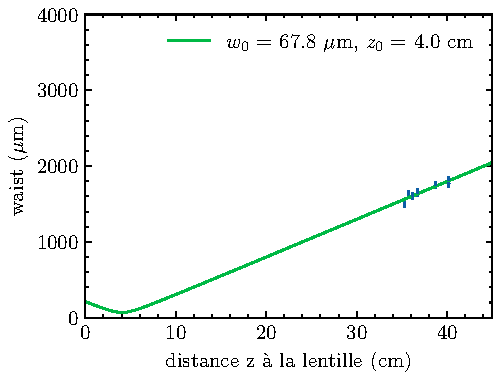
\includegraphics{./img/waist faisceau vert.pdf}
	\caption{Profil du faisceau vert généré}
	\label{fig:vert}
\end{figure}

\section{Étude à haute puissance}
\subsection{Caractérisation à haute puissance}
\subsection{Recherche d'un régime exploitable}
\section{Conclusion}


\setcitestyle{numbers}
\bibliography{rapport.bib}
\bibliographystyle{unsrtnat}

\newpage

\appendix
\section{\'Equation d'onde non-linéaire} 
\label{NL}
Considérons un milieu matériel non magnétique, dans lequel
\begin{align*}
	\v D = \varepsilon_0 \v E + \v P \text{, } \v B = \mu_0 \v H
\end{align*}
où $\v P$ est la polarisation du milieu (induite par le champ dans le milieu supposé sans polarisation propre).

En prenant le rotationnel de l'équation de Maxwell-Faraday et en injectant l'équation de Maxwell-Ampère (sans courant libre), on trouve
\begin{align*}
	\rot (\rot \v E) = \grad (\divg \v E) - \v \nabla^2 \v E = - \frac{1}{c^2} \frac{\partial^2 \v E}{\partial t^2} - \mu_0 \frac{\partial^2 \v P}{\partial t^2} \\
\end{align*}

Le terme $\grad (\divg \v E)$ est nul dans un milieu linéaire isotrope (et sans charges libres) puisque $\divg \v D=0$ implique alors $\divg \v E = 0$, ou encore pour une onde plane transverse. En règle générale, ce terme est non nul à cause de l'anisotropie ou de la non-linéarité du matériau, mais il reste négligeable, en particulier dans l'approximation paraxiale \ncite{boyd}, et sera négligé par la suite.


%terme négligé (angle de double réfraction \cite{joffre}) \cite{boyd}

On décompose ensuite la polarisation en un terme linéaire $\v P^\mathsc{(1)}$ et un terme non linéaire $\v P^\mathsc{NL}$, et de même pour l'induction électrique $\v D = \v D^\mathsc{(1)} + \v D^\mathsc{NL} = \v D^\mathsc{(1)} + \v P^\mathsc{NL}$. 

Comme la réponse du milieu dépend de la fréquence de l'excitation, on décompose les champs en composantes à différentes pulsations $\omega_q$ :
\begin{align*}
	\v E(\v r, t) &= \mathfrak{Re} \left\{ \sum_{q \in \mathbb N} \v {\boldsymbol{\mathcal E}}_q (\v r) \e{-i \omega_q t} \right\} \\
	\v D(\v r, t) &= \mathfrak{Re} \left\{ \sum_{q \in \mathbb N} \v {\boldsymbol{\mathcal D}}_q (\v r) \e{-i \omega_q t} \right\} \\
	\v P^\mathsc{NL}(\v r, t) &= \mathfrak{Re} \left\{ \sum_{q \in \mathbb N} \v {\boldsymbol{\mathcal P}}^\mathsc{NL}_q (\v r) \e{-i \omega_q t} \right\}
\end{align*}

On peut alors écrire $\v {\boldsymbol{\mathcal D}}^\mathsc{(1)}_q = \tens \varepsilon^{\mathsc(1)}(\omega_q) \v {\boldsymbol{\mathcal E}}_q$ avec $\tens \epsilon^{(1)}(\omega_q)$ le tenseur de permittivité diélectrique relative (linéaire) à $\omega_q$, ce qui conduit à l'équation de Helmholtz  \citep{boyd}
\begin{align*}
	\boldsymbol{\nabla}^2 \boldsymbol{\E}_q + \frac{\omega_q^2}{c^2}\tens\epsilon^{(1)}(\omega_q)\cdot \v \E_q(\v r) = - \frac{\omega_q^2}{\epsilon_0 c^2} \boldsymbol{\mathcal{P}}^\mathsc{NL}_q(\v r)
\end{align*}

\section{Validité de l'hypothèse de non déplétion}
\label{ndepl}

\section{Efficacité de conversion dans un  cristal périodiquement pôlé}
Étude par TF dans le plan (cf Dareau)
%Dvpt en série de Fourier de d(z)
\label{BK}


\end{document}

